% !TeX program = xelatex
\documentclass[t, 10pt]{beamer}

\usepackage[brazil]{babel}
\let\latinencoding\relax
\usepackage{fontspec}
\usepackage[T1]{fontenc}
\usepackage{lmodern}

\usepackage{graphicx}
\usepackage{minted, xcolor}
\usepackage{tikz}
\usepackage{cancel}
\usepackage[portuguese, ruled, linesnumbered, noend]{algorithm2e}

\title{Métodos eficientes de ordenação}
\subtitle{Heapsort}
\author{Alessandro Jean \\ \and Igor Neres Trindade}
\institute{Universidade Federal do ABC}
\date{25 de Maio de 2018}


%\usetheme{metropolis}
%\usecolortheme{beaver}
\useoutertheme{metropolis}
\useinnertheme[subsectionpage=simple]{metropolis}
\usefonttheme{metropolis}
\usecolortheme{beaver}
\usefonttheme[onlymath]{serif}

\beamertemplatenavigationsymbolsempty
\setbeamercolor{math text}{fg=black!15!blue}
\setsansfont[BoldFont={Fira Sans SemiBold}, Numbers={OldStyle}]{Fira Sans Book}
\setbeamertemplate{section in toc}[sections numbered]


\definecolor{codeBg}{HTML}{282828}
\definecolor{friendlybg}{HTML}{f0f0f0}
\definecolor{highlightBg}{HTML}{161616}
\usemintedstyle{monokai}
\setminted[c]{
  fontsize=\scriptsize,
  autogobble,
  linenos,
  bgcolor=codeBg,
  highlightcolor=highlightBg
}

%\boldmath

\renewcommand{\thealgocf}{}
\renewcommand{\algorithmcfname}{}
\SetAlgoCaptionSeparator{}
\SetKw{KwDownto}{decrescendo}
\SetKw{KwTo}{até}
\SetKw{KwAnd}{e}

\begin{document}
  \frame[noframenumbering,plain]{\titlepage}	
  
  \begin{frame}[noframenumbering,plain]{Sumário}
    \tableofcontents
  \end{frame}
  
  \section{Introdução}
  
  \begin{frame}{Introdução}
    \begin{itemize}
      \item Inventado por J\@. W\@. J\@. Williams em 1964;
      \item No mesmo ano, Robert W\@. Floyd publicou uma versão aprimorada que ordena
      um vetor in-place;
   	  \item Uso de uma estrutura de dados chamada \emph{heap};
   	  \item Parecido com o \emph{selection sort};
   	  \item Não é considerado um algoritmo estável.
   	  \item Tem complexidade $O(n\log(n))$ no pior caso.
   	  
    \end{itemize}
  \end{frame}

  \section{Heap}
  
  \begin{frame}{Definição}
    \begin{itemize}
      \item Estrutura que utiliza como base um vetor;
      \item Pode ser visto como uma árvore binária;
      \item Cada elemento no vetor corresponde a um nó da árvore;
      \item Alguns livros implementam uma versão para vetores \texttt{[1..n]}.
      Neste caso, será adotada a versão \texttt{[0..n - 1]}.
    \end{itemize}

    \pause
    \begin{center}
      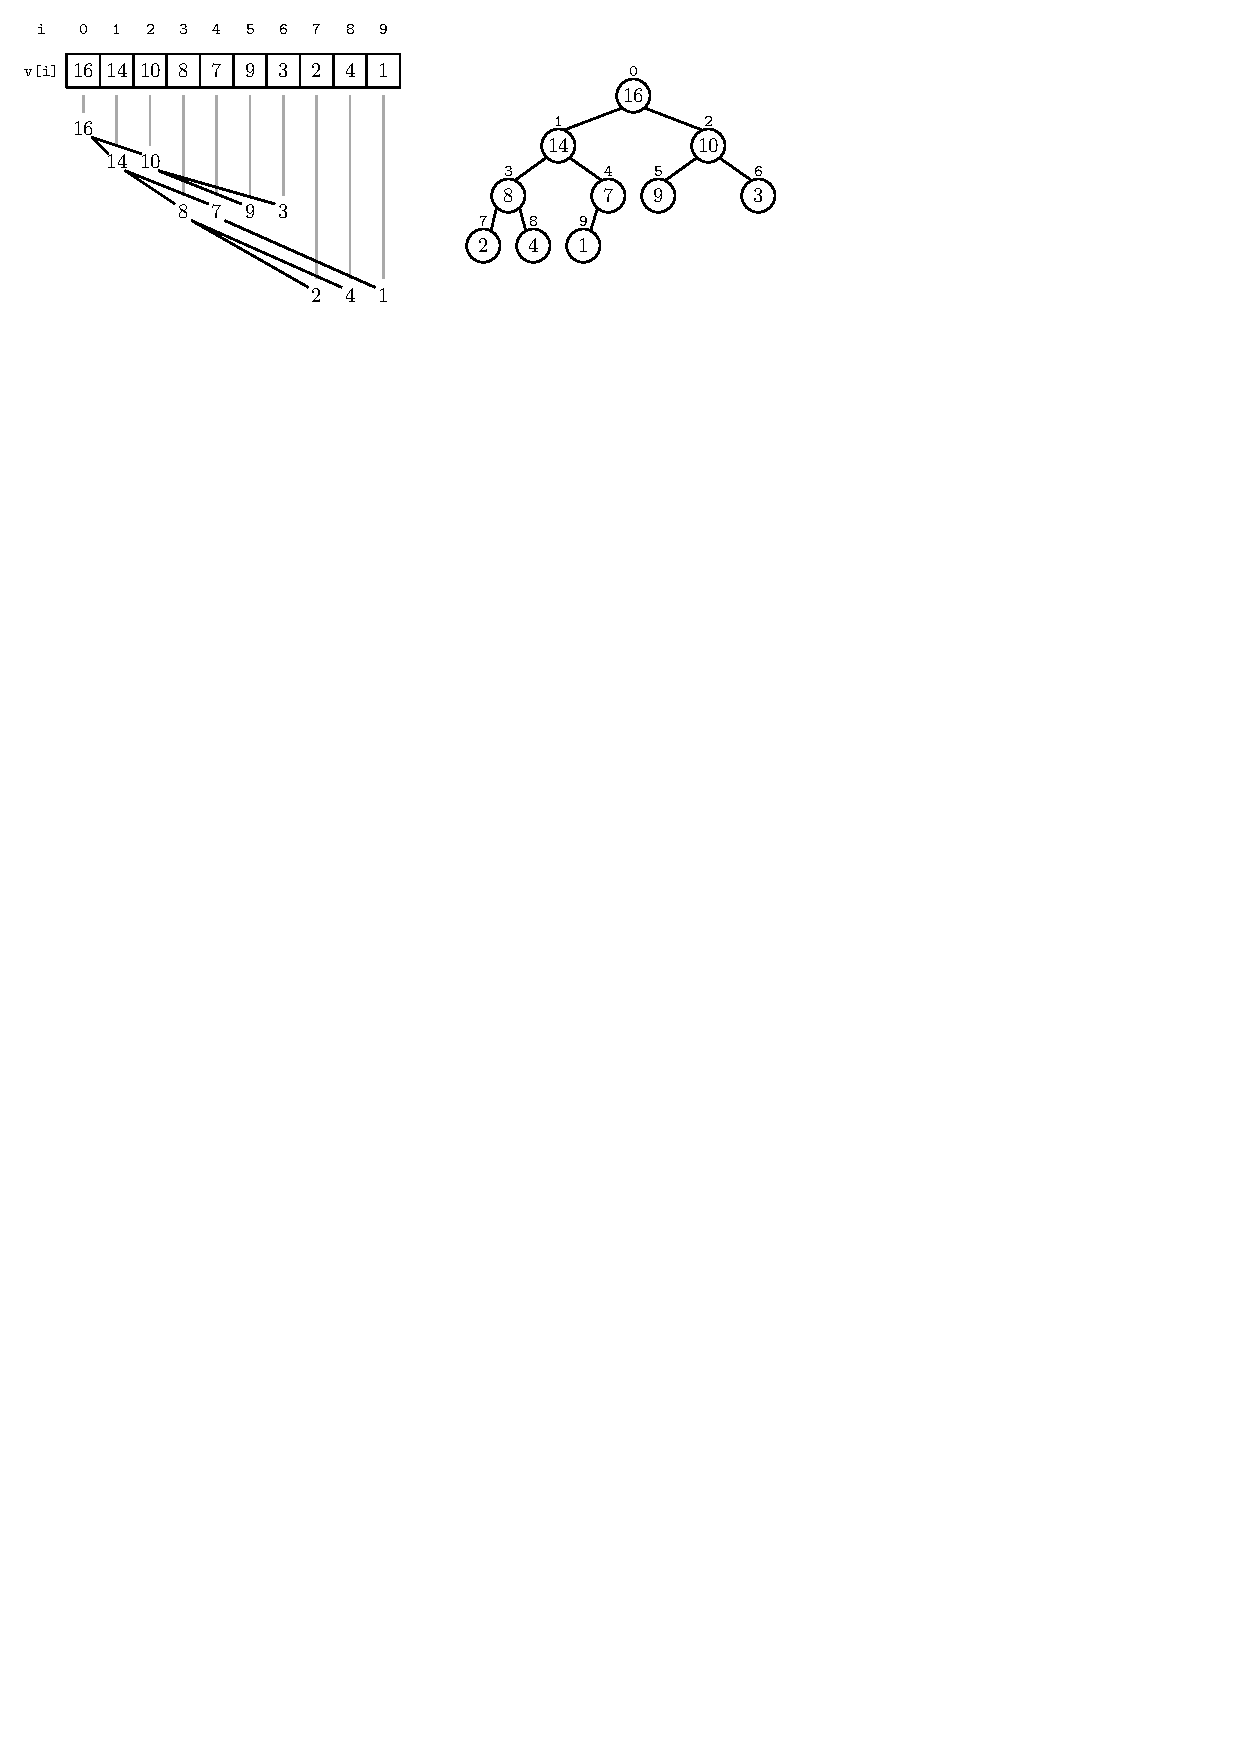
\includegraphics[width=\textwidth]{img/img31.pdf}
      {\footnotesize
        \emph{Heap} máximo representado por um vetor e uma árvore 
        binária completa. 
      } 
    \end{center}
  \end{frame}

  \begin{frame}{Definição}
    Dado uma árvore binária de altura $h$:
    \begin{itemize}
      \item Uma árvore binária \textbf{cheia} é aquela em que cada
      nó até o nível $h - 1$ possui exatamente dois filhos, e os
      nós no nível $h$ não possuem filhos, ou seja, são as folhas.
      \item<2> Uma árvore binária \textbf{completa} é aquela que possui
      todos os níveis preenchidos, exceto possivelmente o último,
      que é preenchido da esquerda para a direita.
    \end{itemize}

    \begin{center}
      \begin{onlyenv}<1>
        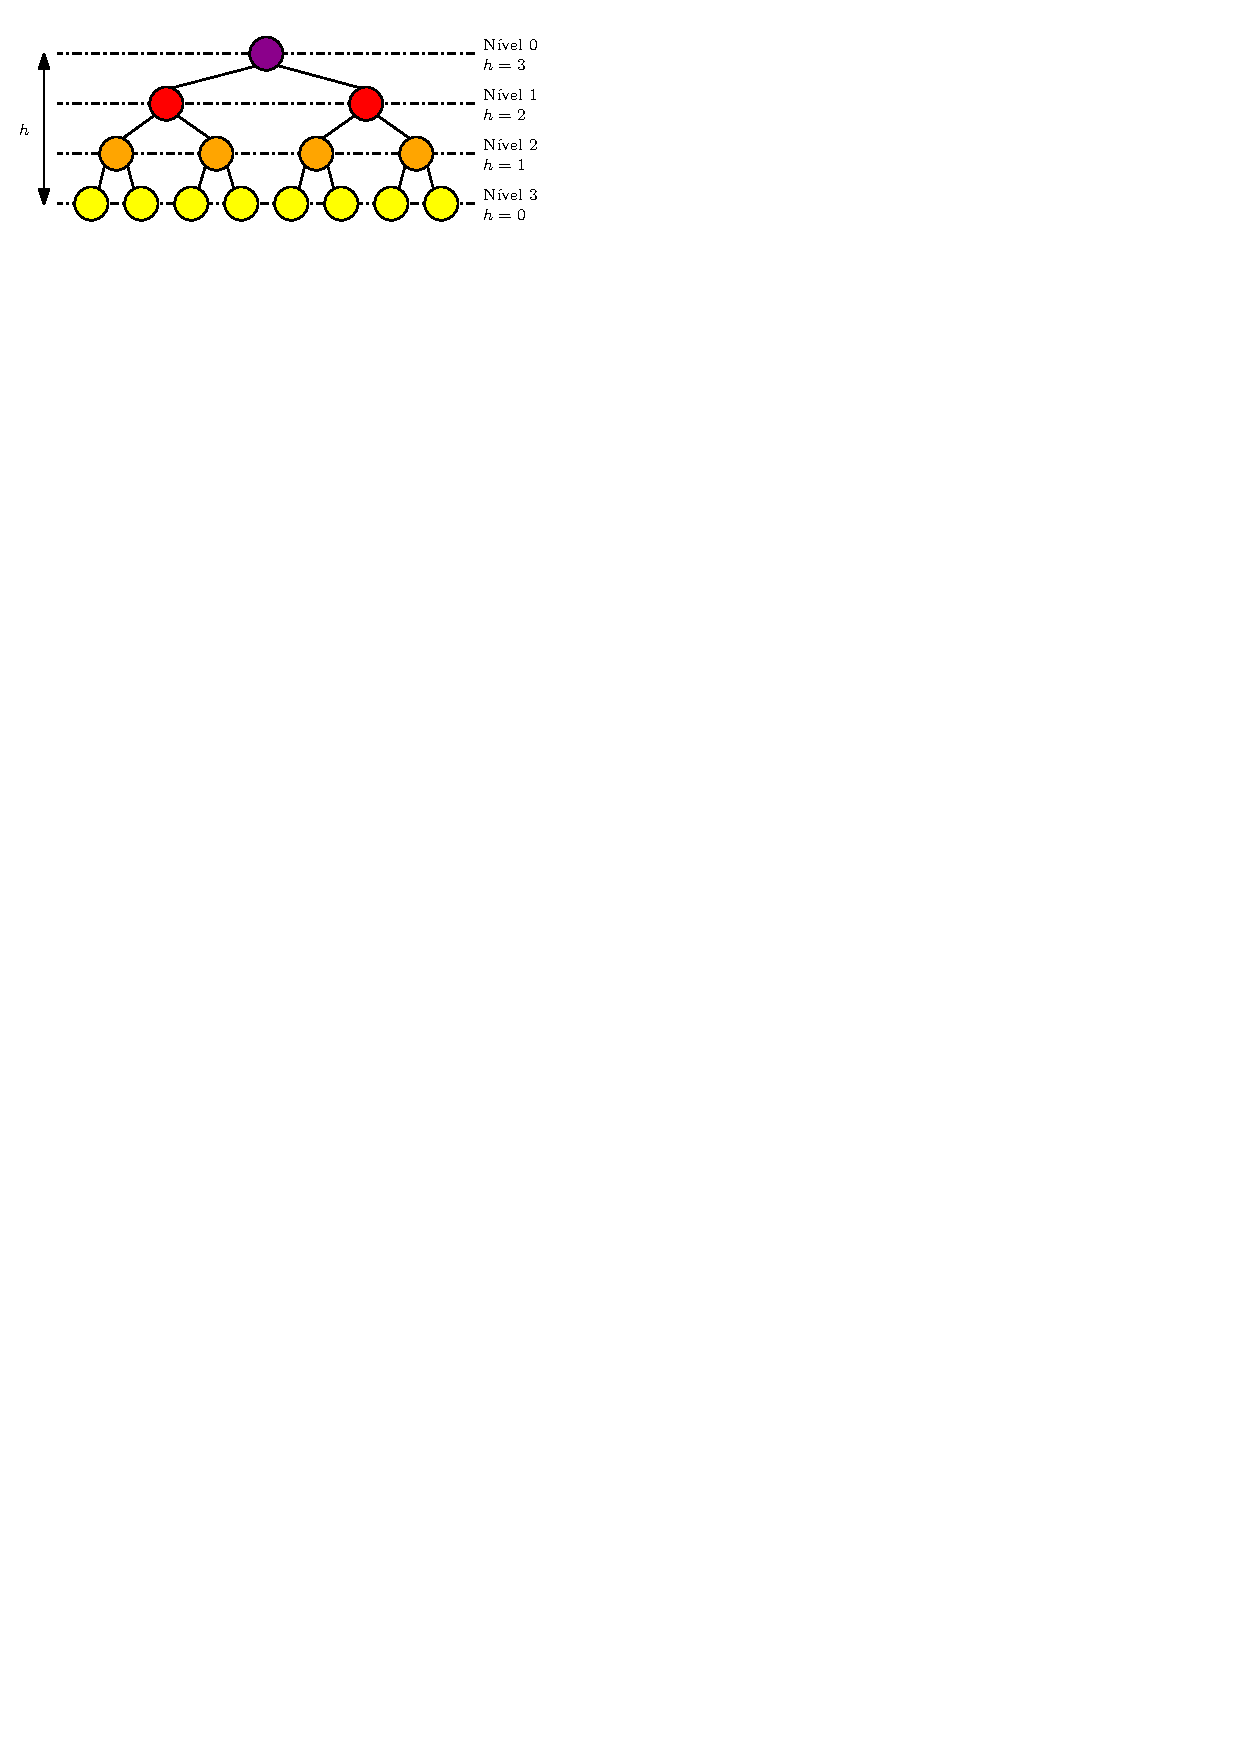
\includegraphics[]{img/img32.pdf}

        {\footnotesize
          Árvore binária cheia.
        }
      \end{onlyenv}
      \begin{onlyenv}<2>
        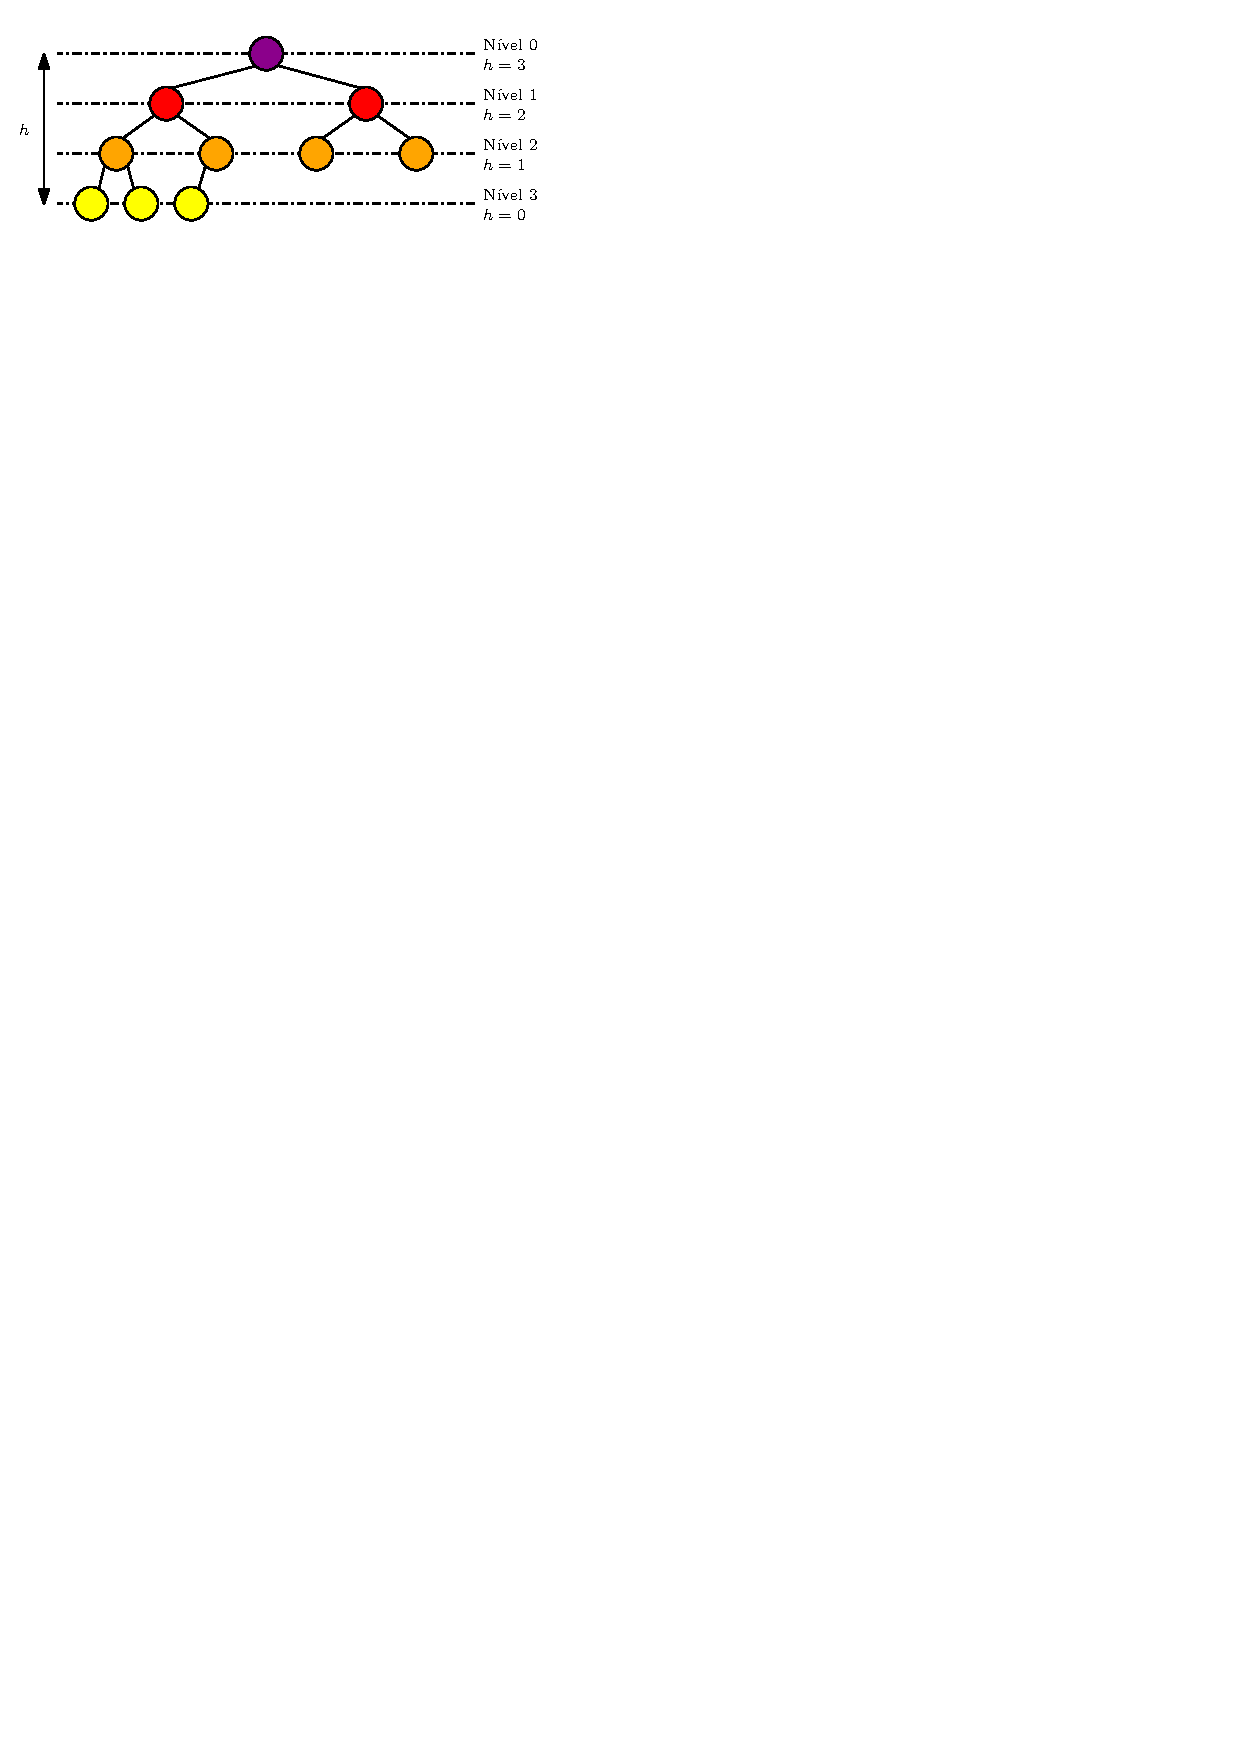
\includegraphics[]{img/img33.pdf}

        {\footnotesize
          Árvore binária completa.
        }
      \end{onlyenv}
    \end{center}
  \end{frame}

  \subsection{Relações}

  \begin{frame}[fragile]{Relações}
    Seja uma árvore binária completa representada por um 
    vetor \texttt{v[0..n - 1]}.
    \begin{center}
      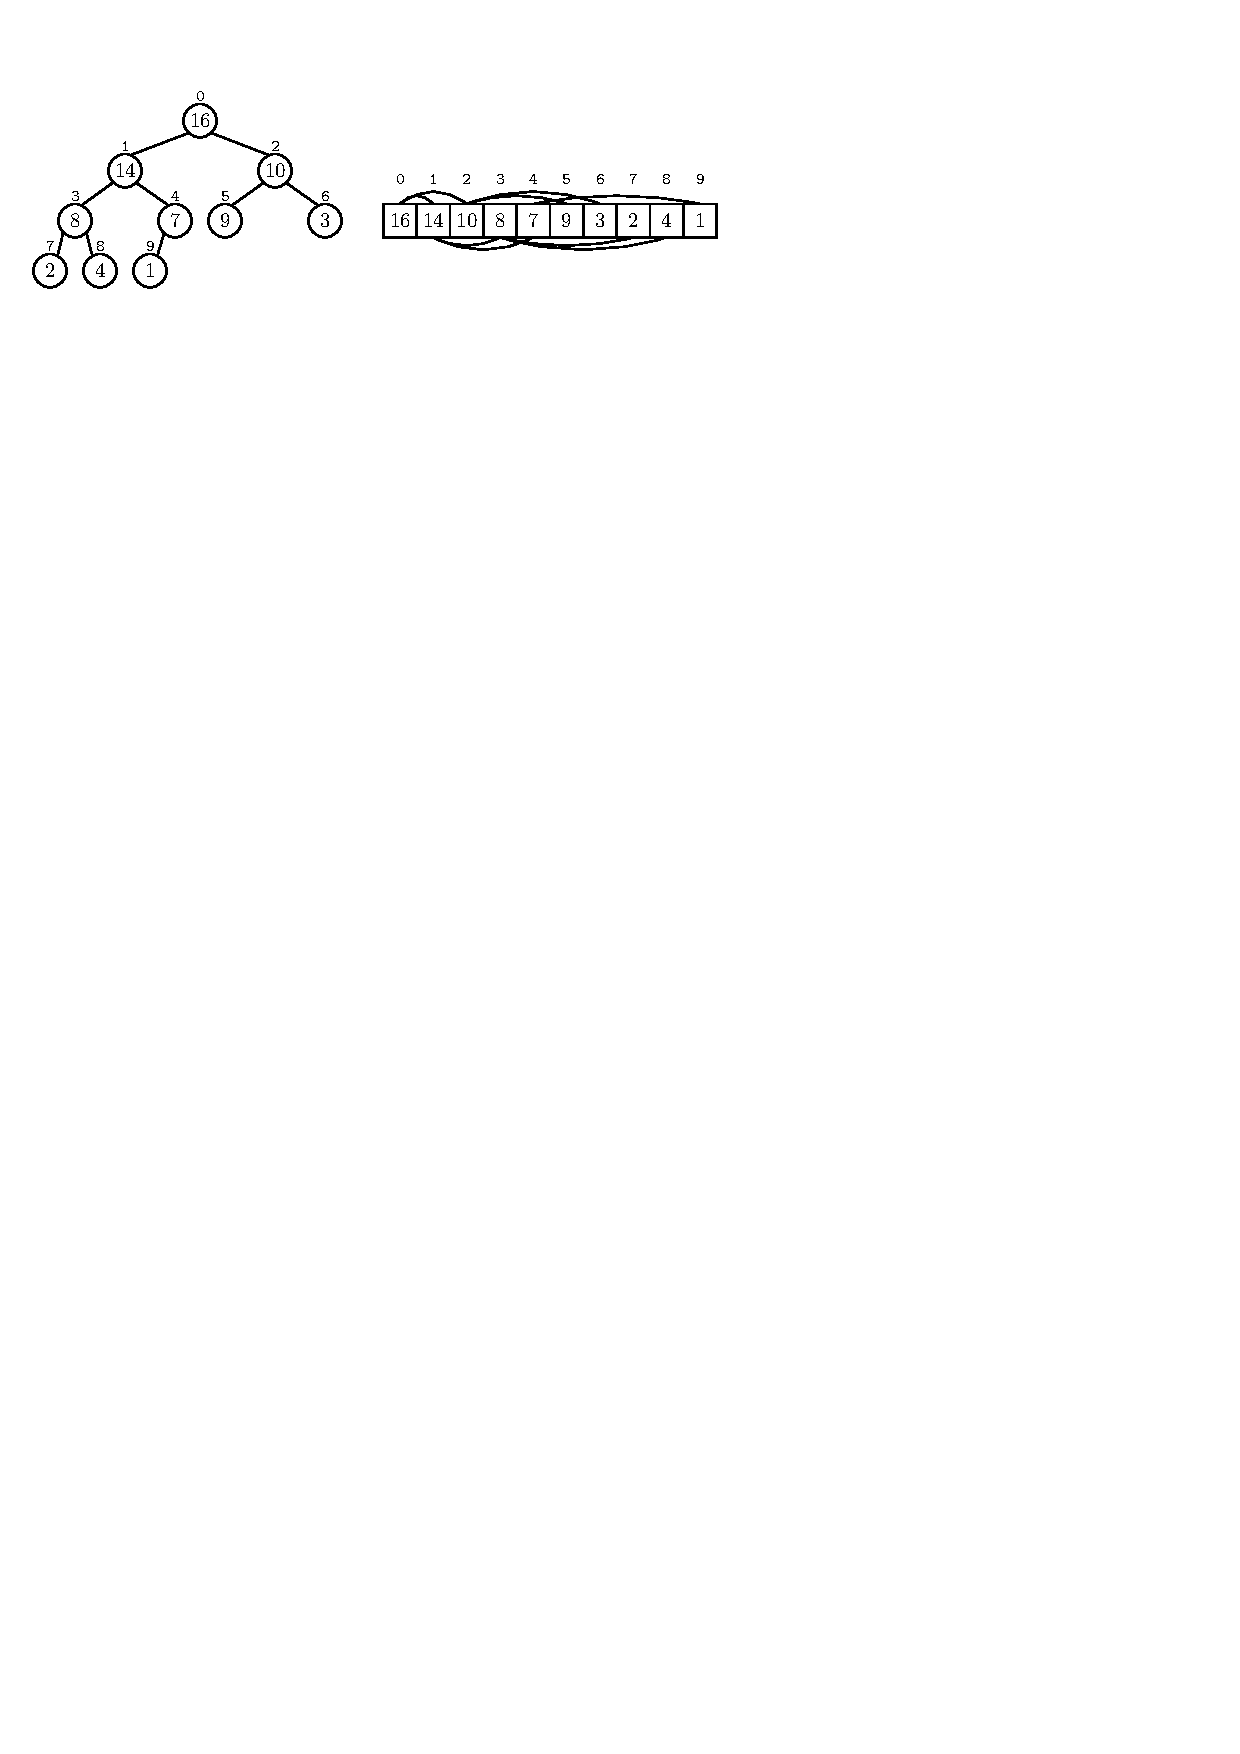
\includegraphics[width=\textwidth]{img/img1.pdf}
    \end{center}
    \begin{onlyenv}<1>
      \begin{itemize}
        \item Para qualquer índice ou nó $i$:
        \begin{itemize}
            \item O pai de $i$ é $\left\lfloor\frac{i - 1}{2}\right\rfloor$.
            \item O filho esquerdo de $i$ é $2i + 1$.
            \item O filho direito de $i$ é $2i + 2$.
        \end{itemize}
        \item O nó \texttt{v[0]} não tem pai, sendo o nó raiz;
      \end{itemize}
    \end{onlyenv}
    \begin{onlyenv}<2>
      \vspace{-1em}
      \begin{center}
      \begin{minipage}{0.6\textwidth}
      \begin{minted}{c}
      int left (int i) { return 2 * i + 1; }
      
      int right (int i) { return 2 * i + 2; }
      
      int parent (int i) { return (i - 1) / 2; }
      \end{minted}
      \end{minipage}
      \end{center}
    \end{onlyenv}
    \begin{onlyenv}<3>
      \begin{itemize}
        \item Um nó $i$ tem filho esquerdo se $2i + 1 < n$;
        \item Um nó $i$ tem filho direito se $2i + 2 < n$;
        \item Um nó $i$ é um nó folha se $2i + 1 \geq n$.
      \end{itemize}
    \end{onlyenv}
    \begin{onlyenv}<4>
      \vspace{-1em}
      \begin{center}
      \begin{minipage}{0.8\textwidth}
      \begin{minted}{c}
      int hasLeftChild (int i, int n) { return left(i) < n; }
      
      int hasRightChild (int i, int n) { return right(i) < n; }
      
      int isLeaf (int i, int n) { return left(i) >= n; }
      \end{minted}
      \end{minipage}
      \end{center}
    \end{onlyenv} 
  \end{frame}

  \subsection{Tipos}
  
  \begin{frame}{Tipos}
    \begin{itemize}
      \item Existem dois tipos de \emph{heaps};
      \item Cada um satisfaz uma \textbf{propriedade de \emph{heap}};
      \item<2-> \textbf{\emph{Heap} máximo:} o maior elemento é a raiz e as sub-árvores possuem valores
      menores ou iguais que o pai, ou seja, \texttt{v[parent(i)] >= v[i]};
      \item<3-> \textbf{\emph{Heap} mínimo:} o menor elemento é a raiz e as sub-árvores possuem valores
      maiores ou iguais que o pai, ou seja, \texttt{v[parent(i)] <= v[i]};
    \end{itemize}
  \end{frame}
  
  \subsection{Manutenção}
  
  \begin{frame}{Manutenção}
    Muitas vezes, um \emph{heap} não vai estar cumprindo sua propriedade de seu tipo, portanto é preciso
    realizar a manutenção.
    
    \setbeamercolor{math text}{fg=black}
    \begin{center}
    \begin{minipage}{0.75\textwidth}
    \begin{algorithm}[H]
      \caption{\textsc{Max-Heapify}$(v, n, i)$}
      $e \leftarrow \textsc{LEFT}(i)$  \\
      $d \leftarrow \textsc{RIGHT}(i)$ \\
      $maior \leftarrow i$ \\
      \Se{$\textsc{Has-Left-Child}(i,n)$ \KwAnd $v[maior] > v[i]$}{
        $maior \leftarrow e$
      }
      \Se{$\textsc{Has-Right-Child}(i,n)$ \KwAnd $v[maior] > v[i]$}{
        $maior \leftarrow d$
      }
      \Se{$maior \neq i$}{
        $v[i] \leftrightarrow v[maior]$ \\
        $\textsc{Max-Heapify}(v, n, maior)$
      }
    \end{algorithm}
    \end{minipage}
    \end{center}
  \end{frame}
  
  
  \begin{frame}{Manutenção do \emph{heap} - Exemplo}    
    \begin{figure}[h!]
    \begin{tikzpicture}
       \node<1> (i1) {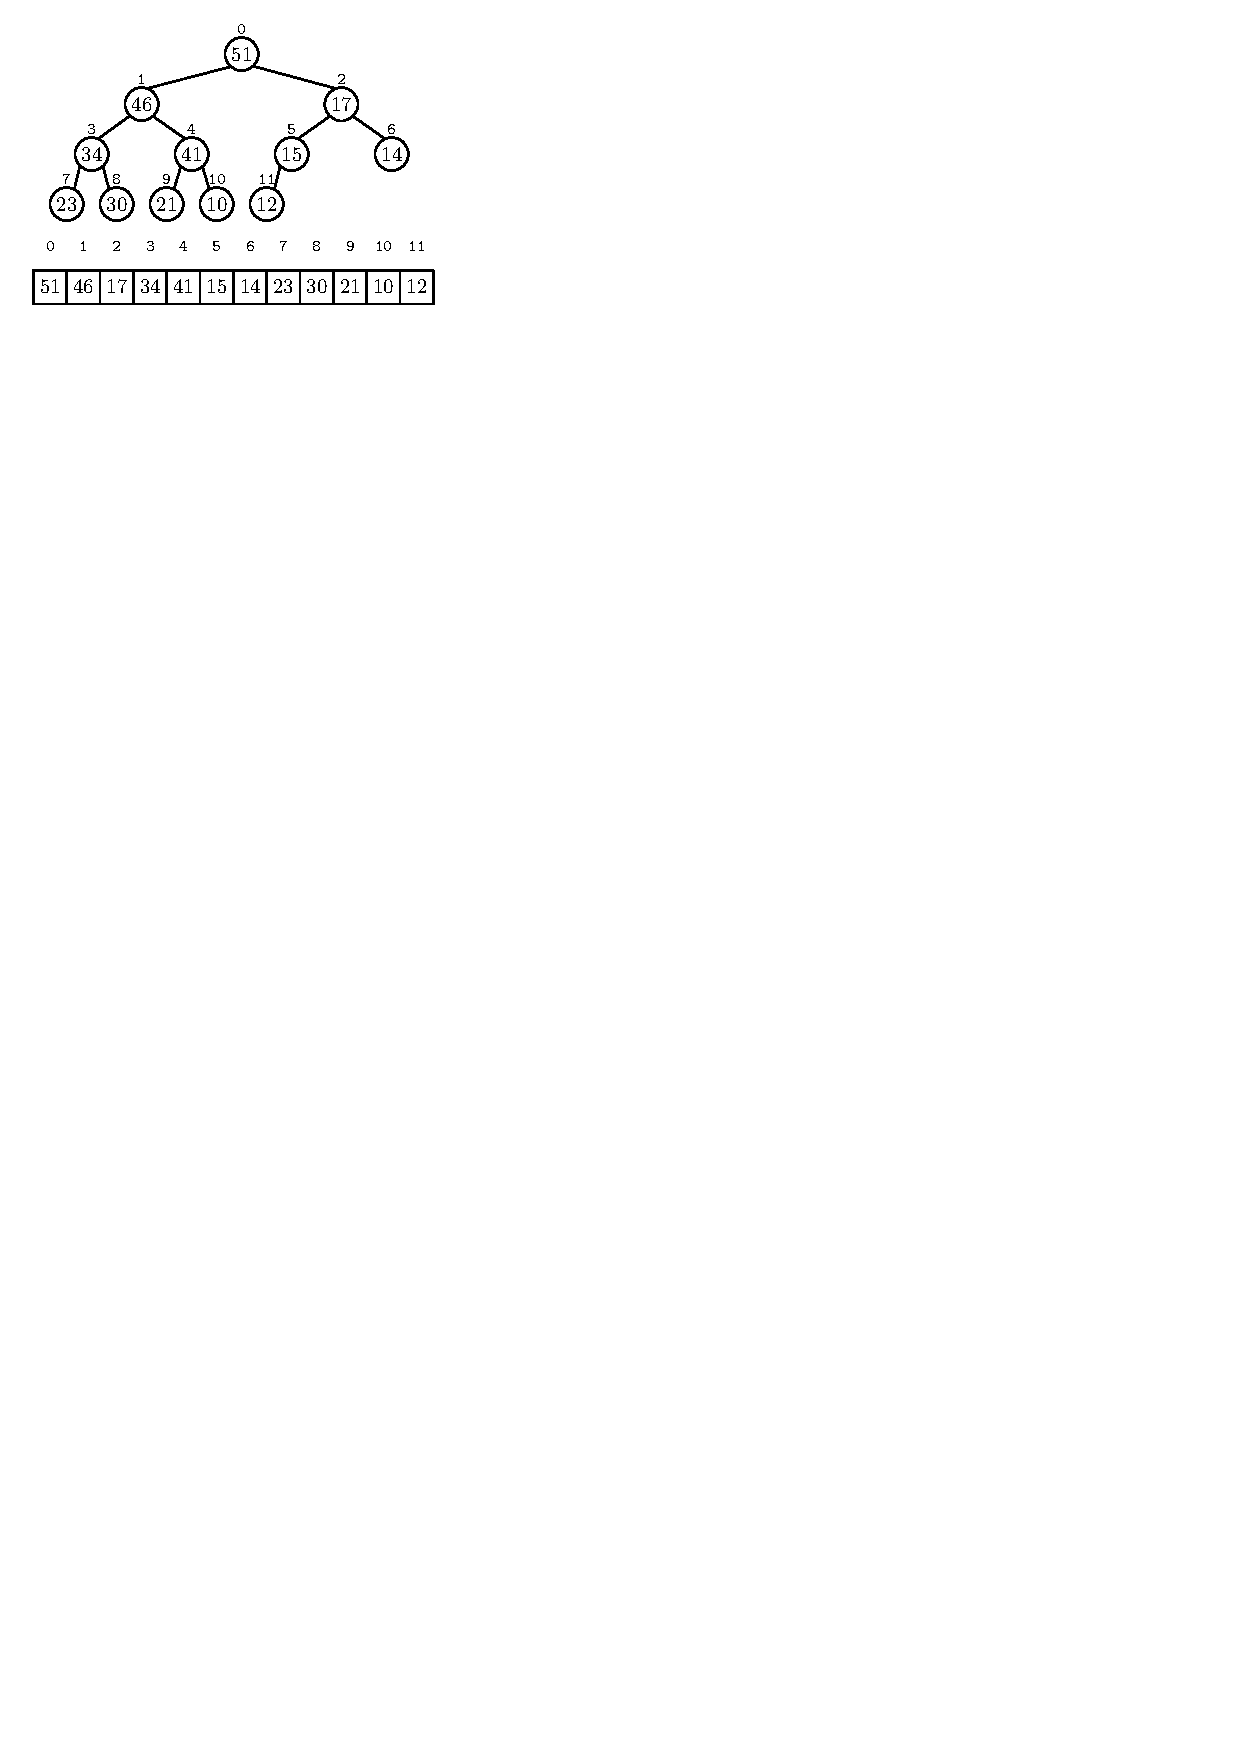
\includegraphics[width=0.75\textwidth]{img/img2.pdf}};
       \node<2> (i2) {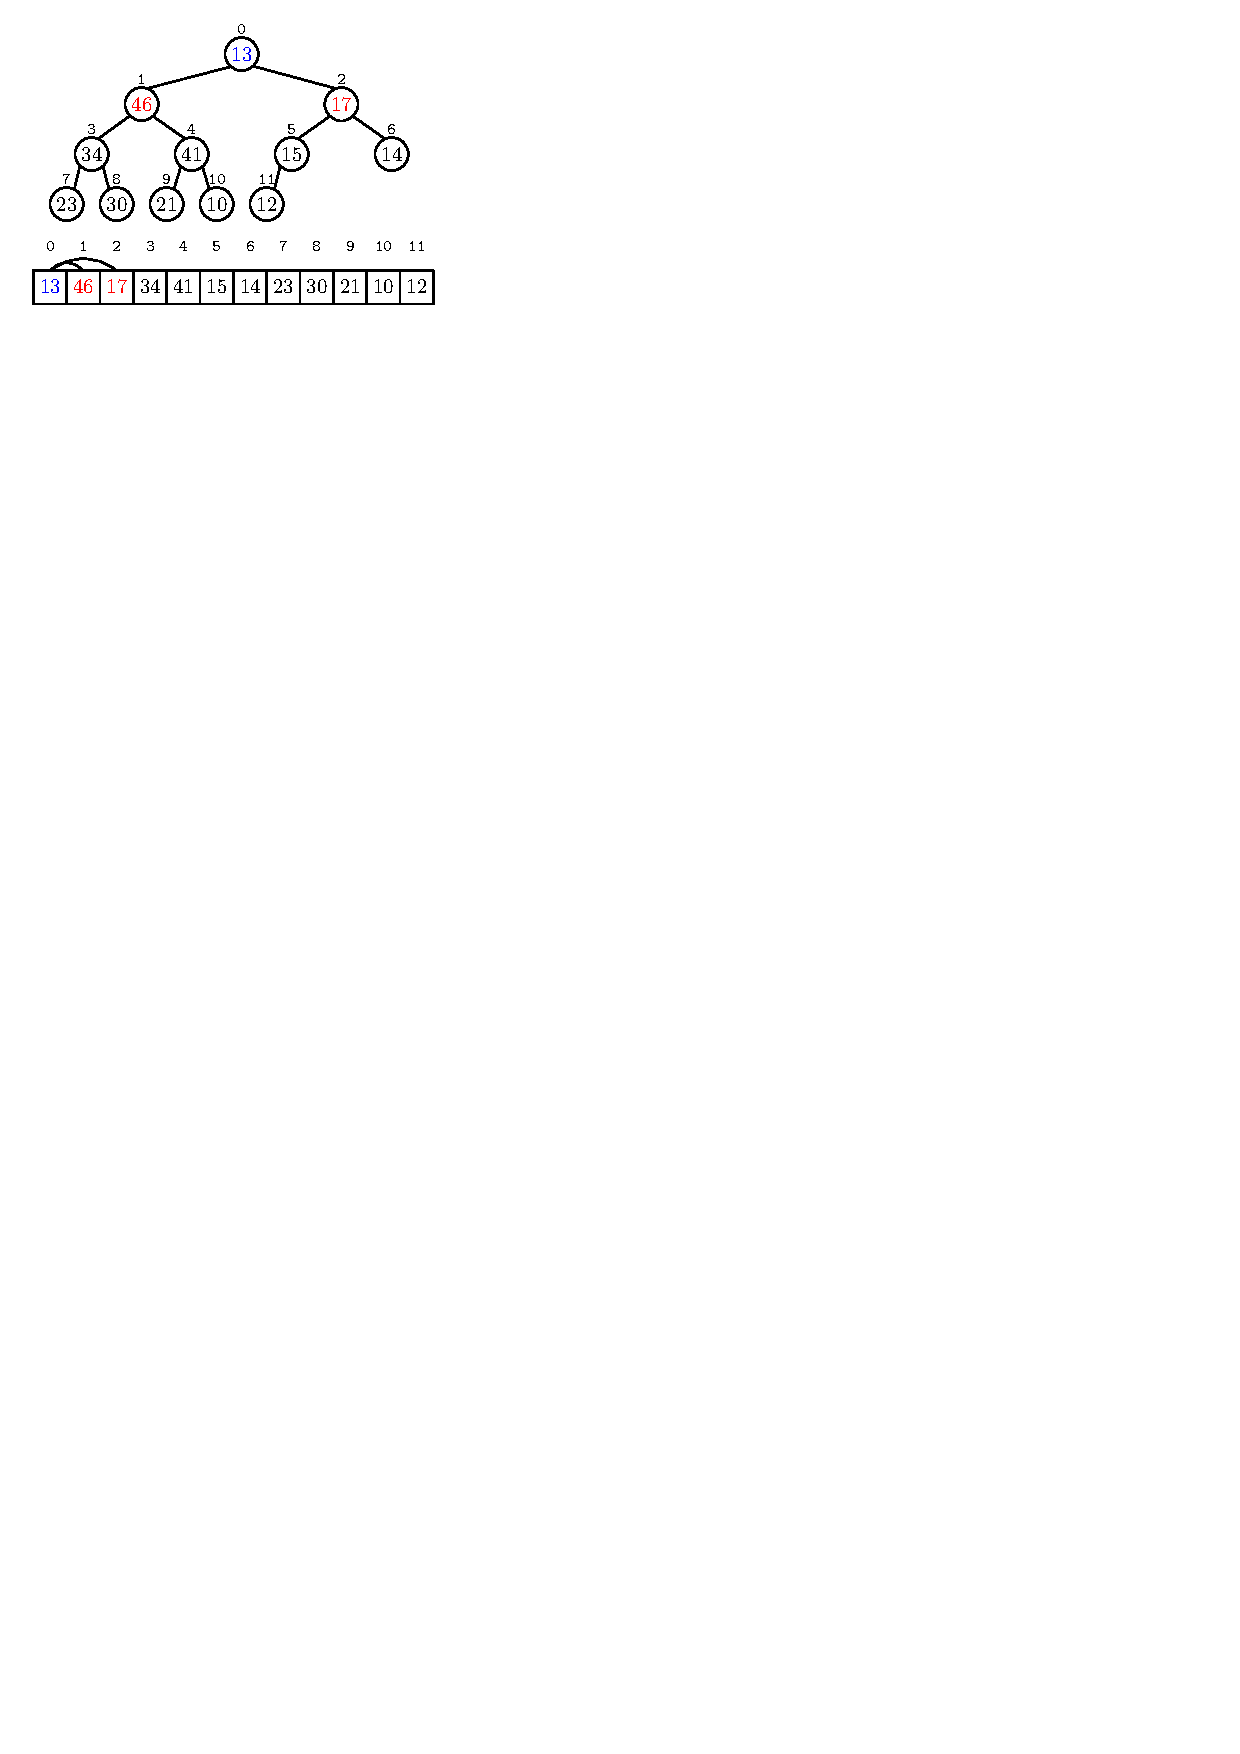
\includegraphics[width=0.75\textwidth]{img/img3.pdf}};
       \node<3> (i3) {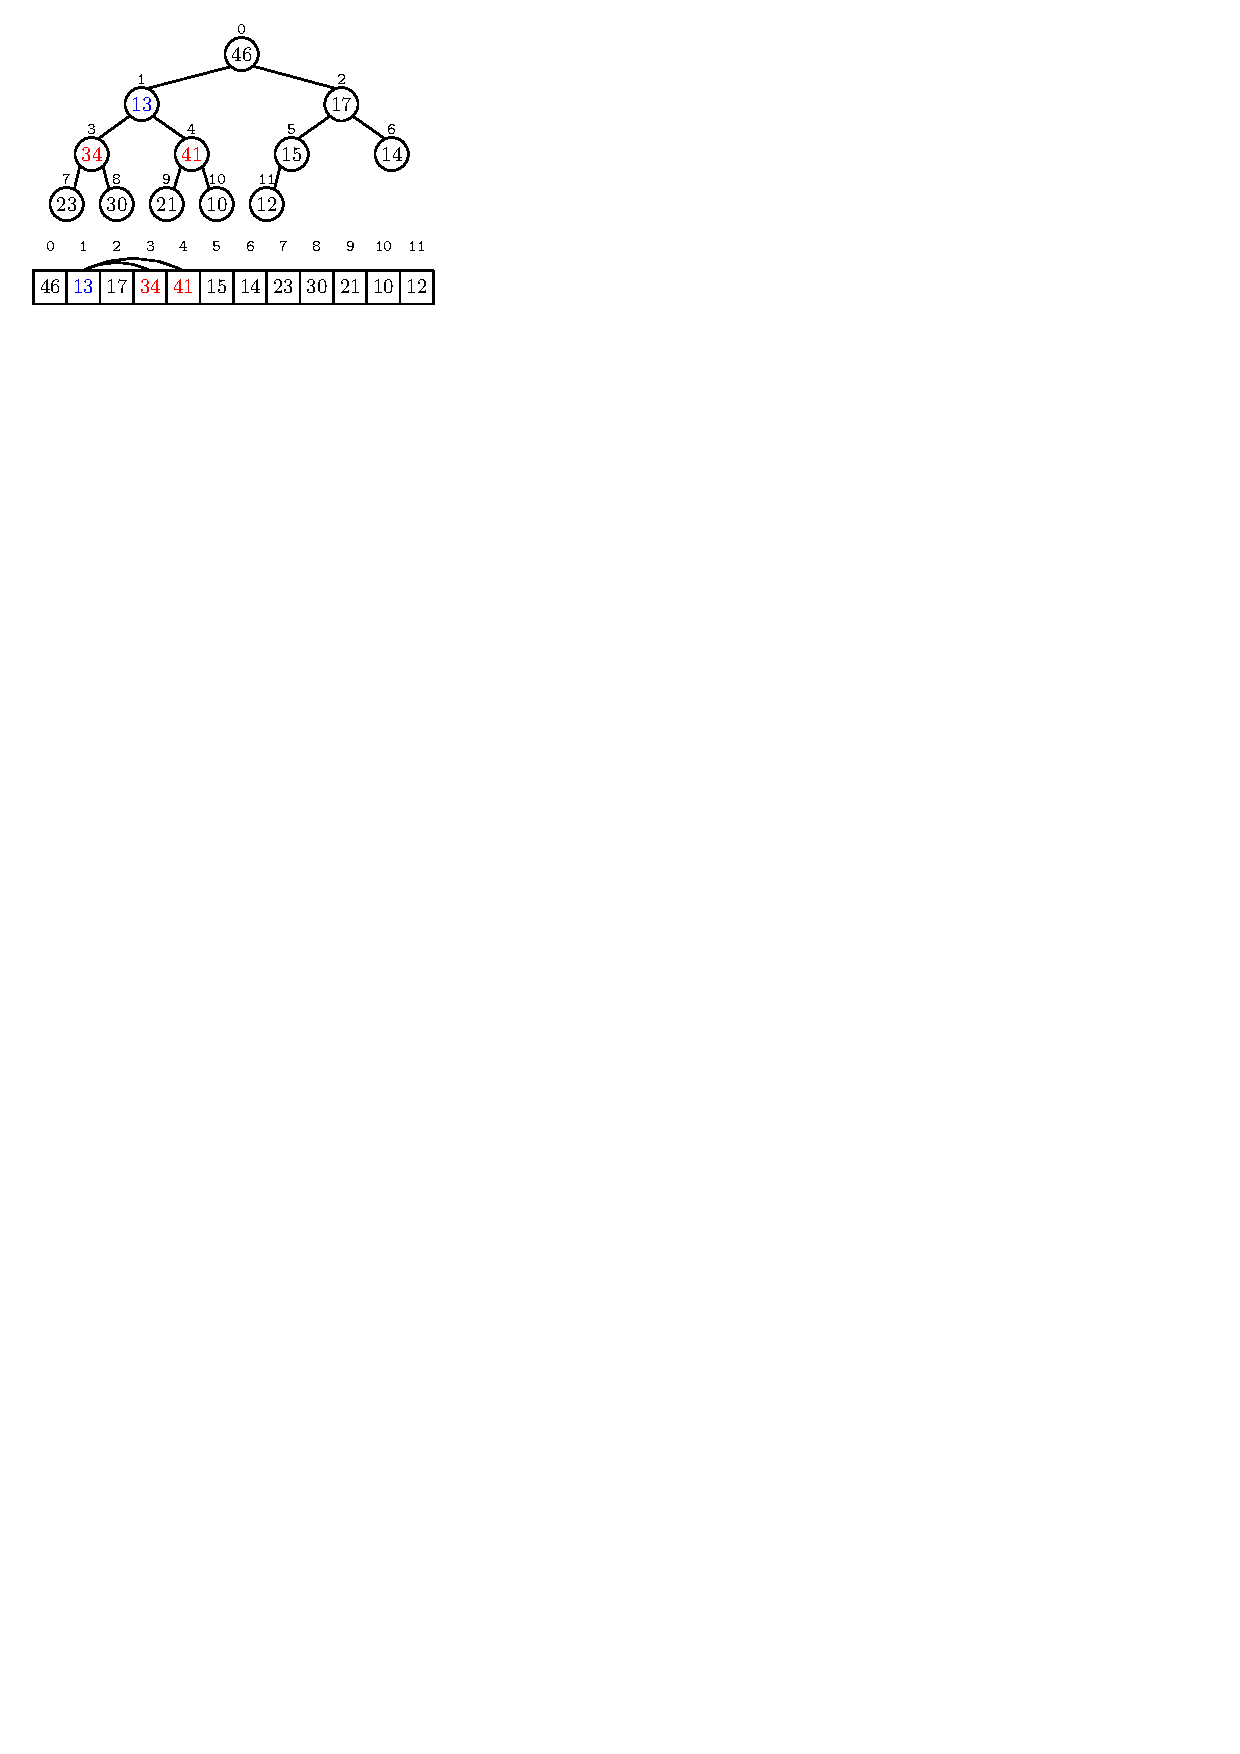
\includegraphics[width=0.75\textwidth]{img/img4.pdf}};
       \node<4> (i4) {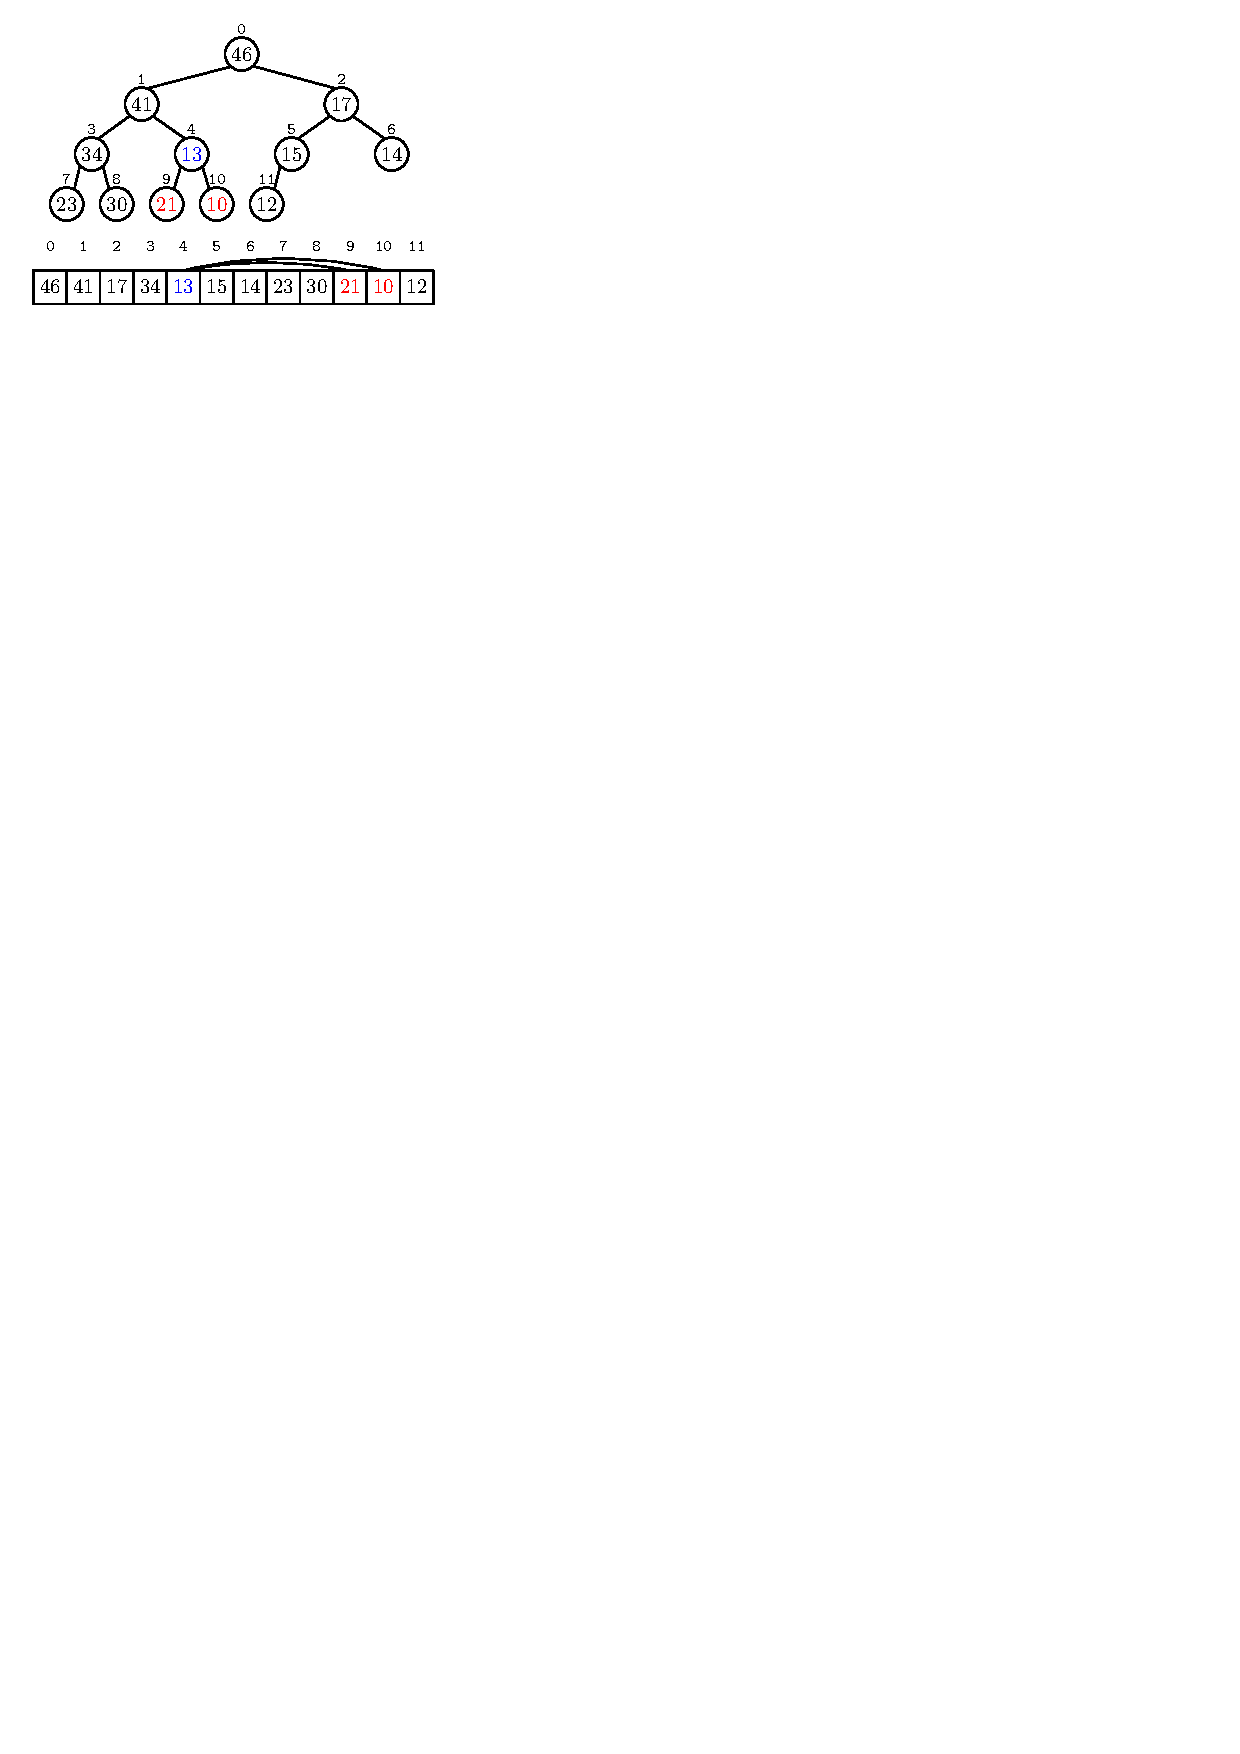
\includegraphics[width=0.75\textwidth]{img/img5.pdf}};
       \node<5> (i5) {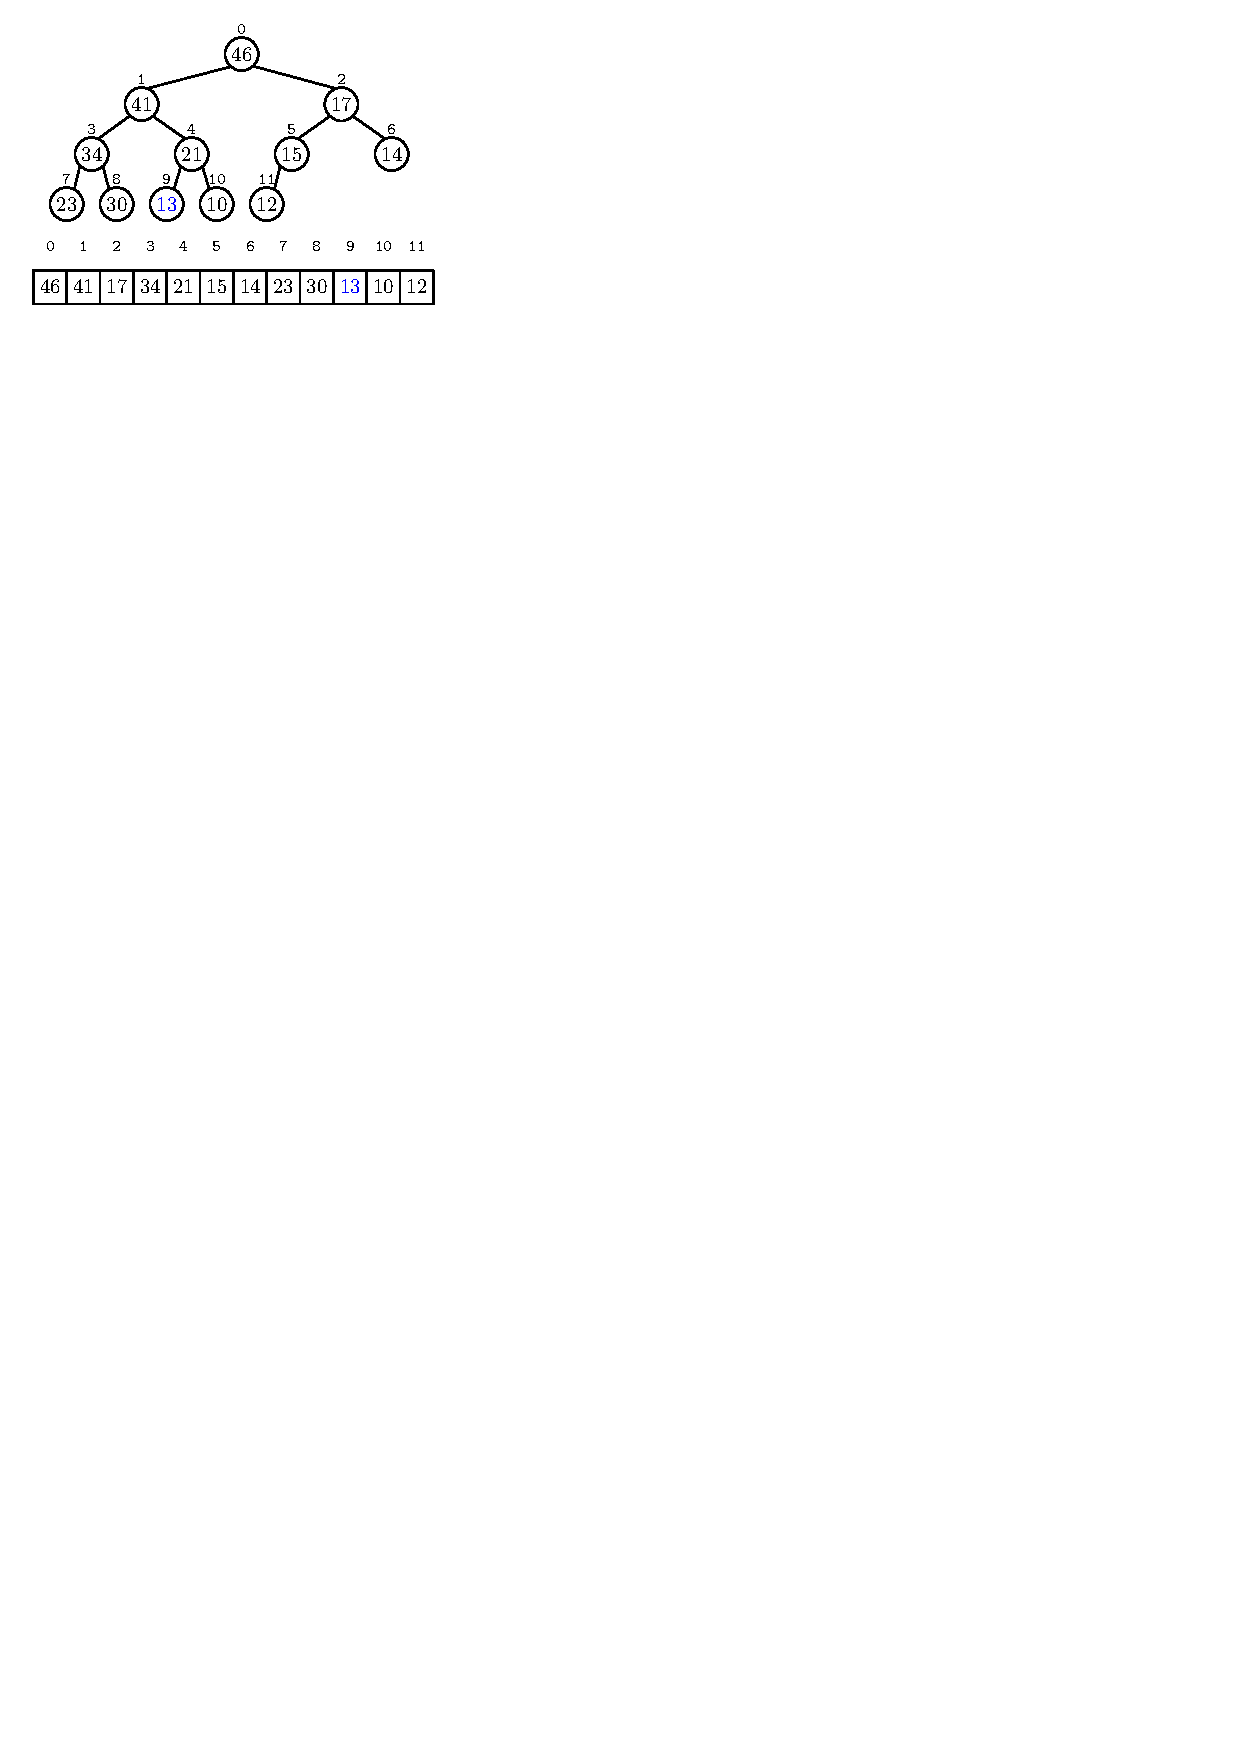
\includegraphics[width=0.75\textwidth]{img/img6.pdf}};
       \node<6> (i6) {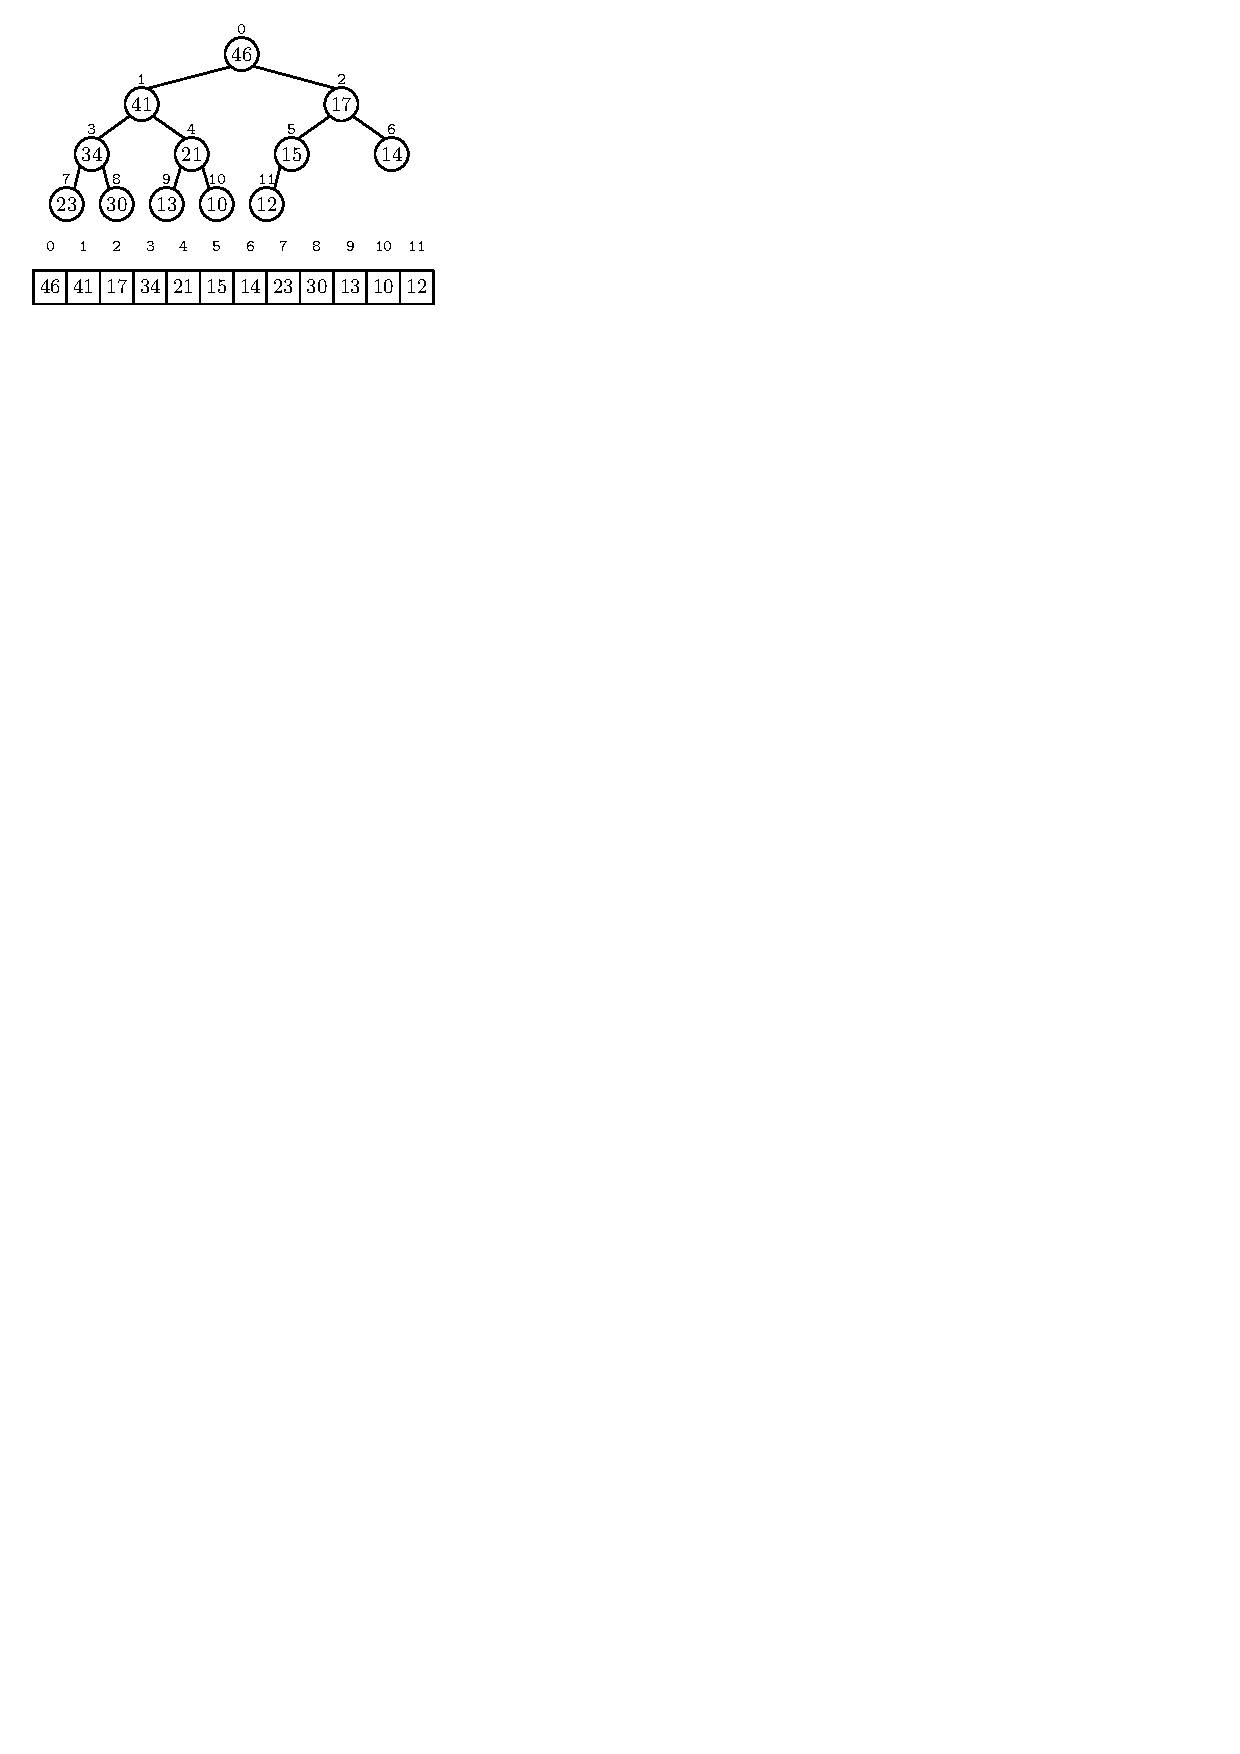
\includegraphics[width=0.75\textwidth]{img/img7.pdf}};
    \end{tikzpicture}
    \end{figure}
  \end{frame}

  \begin{frame}[fragile]{Max-Heapify}
    Recebe \texttt{v[0..n - 1]} e \texttt{i >= 0} tal que as sub-árvores da esquerda e direita
    são \emph{heaps} máximos e rearranja \texttt{v} de modo que a raiz \texttt{i} seja um
    \emph{heap} máximo.
    
    \vspace{-1em}
    \begin{center}
    \begin{minipage}{0.72\textwidth}
    \only<2>{\setminted{highlightlines=4-5}}
    \only<3>{\setminted{highlightlines=7-8}}
    \only<4>{\setminted{highlightlines=10}}
    \only<5>{\setminted{highlightlines=11-13}}
    \only<6>{\setminted{highlightlines=15}}
    \begin{minted}{c}
    int maxHeapify (int * v, int n, int i) {
      int l = left(i), r = right(i), max = i, comp = 1;
      
      if (hasLeftChild(i, n) && v[l] > v[max])
        max = l;
      
      if (hasRightChild(i, n) && v[r] > v[max])
        max = r;
        
      if (max != i) {
        int aux = v[i];
        v[i] = v[max];
        v[max] = aux;
        
        comp += maxHeapify(v, n, max);
      }
      
      return comp;
    }
    \end{minted}
    \end{minipage}
    \end{center}
  \end{frame}

  \begin{frame}{Max-Heapify - Análise de custo}
    Dado uma árvore com $n$ nós, e um dado nó $i$:
    
    \begin{itemize}
      \item Para corrigir os relacionamentos entre \texttt{v[i]}, \texttt{v[left(i)]} e \texttt{v[right(i)]},
      tem-se custo $\Theta(1)$ mais o tempo de execução de \texttt{maxHeapify} em uma das sub-árvores de $i$;
      \item As sub-árvores têm tamanho máximo igual a $\frac{2n}{3}$ \footnotemark[1];
      \item O caso pior ocorre quando a última linha da árvore está exatamente metade cheia \footnotemark[2].
    \end{itemize}

    Pode-se, então, descrever a recorrência de \texttt{maxHeapify} como: $$T(n) = T\left(\frac{2n}{3}\right) + \Theta(1)$$
  
    \footnotetext[1]{
      Mais detalhes: \url{https://bit.ly/2HnTJg9}
    }
    \footnotetext[2]{
      Mais detalhes: \url{https://bit.ly/2HNJnp8}
    }
  \end{frame}

  \begin{frame}{Max-Heapify - Caso pior}
    $$T(n) = T\left(\frac{2n}{3}\right) + \Theta(1)$$
    
    Relembrando o Teorema Mestre: $T(n) = aT\left(\frac{n}{b}\right) + f(n)$
    
    \begin{enumerate}
      \item $f(n) = O(n^{\log_b(a) - \varepsilon}) \Rightarrow T(n) = \Theta(n^{\log_b(a)})$
      \item $f(n) = \Theta(n^{\log_b(a)}) \Rightarrow T(n) = \Theta(n^{\log_b(a)}\log(n))$
      \item $f(n) = \Omega(n^{\log_b(a) + \varepsilon})$ e existe $c < 1$ tal que para todo $n$
      suficientemente grande $af\left(\frac{n}{b}\right) \leq cf(n) \Rightarrow T(n) = \Theta(f(n))$
    \end{enumerate}

    \pause
    \vspace{2em}

    Neste caso, $a = 1$, $b = \frac{3}{2}$, $n^{\log_b(a)} = n^0 = 1$, $f(n) = \Theta(1)$.
    
    Logo, pelo caso 2, $T(n) = \Theta(\log(n))$.
  \end{frame}

  \subsection{Construção}
  
  \begin{frame}[fragile]{Último pai}  
    Dado um \emph{heap} representado por um vetor \texttt{v[0..n - 1]},
    o último pai, ou seja, o último que não é folha, de \texttt{v} é 
    $\left\lfloor\frac{n}{2}\right\rfloor - 1$.
    
    \vspace{-1em}
    \begin{center}
    \begin{minipage}{0.35\textwidth}
    \begin{minted}{c}
    int lastParent (int n) {
      return (n / 2) - 1;
    }
    \end{minted}
    \end{minipage}
    \end{center}
    
    \vspace{-1.5em}
    
    \begin{figure}[h!]
      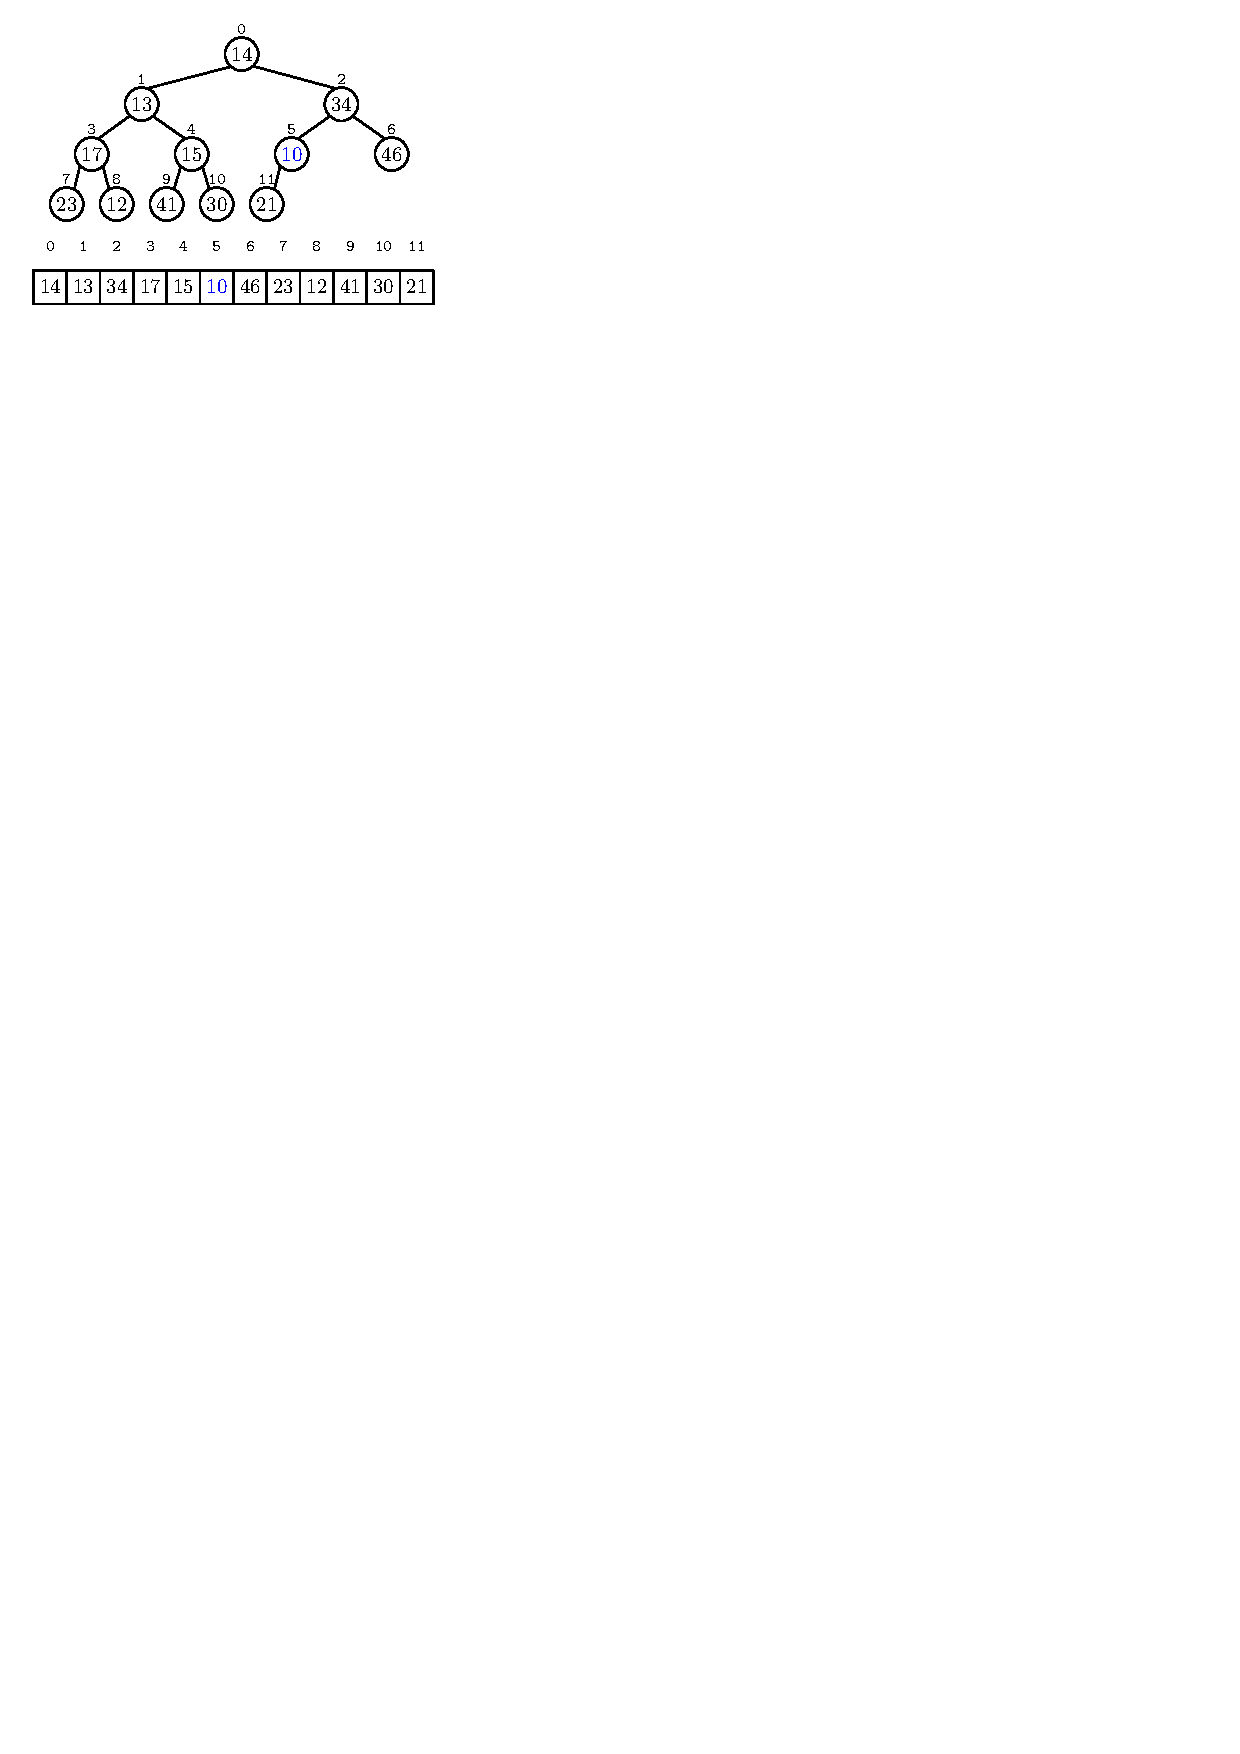
\includegraphics[width=0.6\textwidth]{img/img18.pdf}
    \end{figure}

    \vspace{-0.5em}
    Neste exemplo, $n = 12$, portanto: 
    $\left\lfloor\frac{12}{2}\right\rfloor - 1 = 6 - 1 = 5$.
  \end{frame}

  \begin{frame}{Construção de um \emph{heap} máximo}
    \setbeamercolor{math text}{fg=black}
    \begin{center}
    \begin{minipage}{0.57\textwidth}
    \begin{algorithm}[H]
      \caption{$\textsc{Build-Max-Heap}(v,n)$}
      $lp \leftarrow \textsc{Last-Parent}(n)$ \\
      \Para{$i \leftarrow lp$ \KwDownto \KwTo $0$}{
        $\textsc{Max-Heapify}(v,n,i)$
      }
    \end{algorithm}
    \end{minipage}
    \end{center}
    \setbeamercolor{math text}{fg=black!15!blue}

    É importante começar do último pai até o primeiro, para fazer com
    que o \emph{heap} fique correto e respeite a propriedade de seu tipo. \footnotemark
    
    Caso isso não seja respeitado, pode ocorrer de certas sub-árvores não serem checadas
    e não estejam respeitando a propriedade, fazendo com que o primeiro nó não necessariamente
    seja o maior (ou menor) do \emph{heap}.
    
    \footnotetext[1]{Mais detalhes: \url{https://bit.ly/2qMGbzE}}
  \end{frame}
  
  \begin{frame}{Construção de um \emph{heap} máximo - Exemplo}
    \begin{figure}[h!]
      \begin{tikzpicture}
        \node<1> (i1) {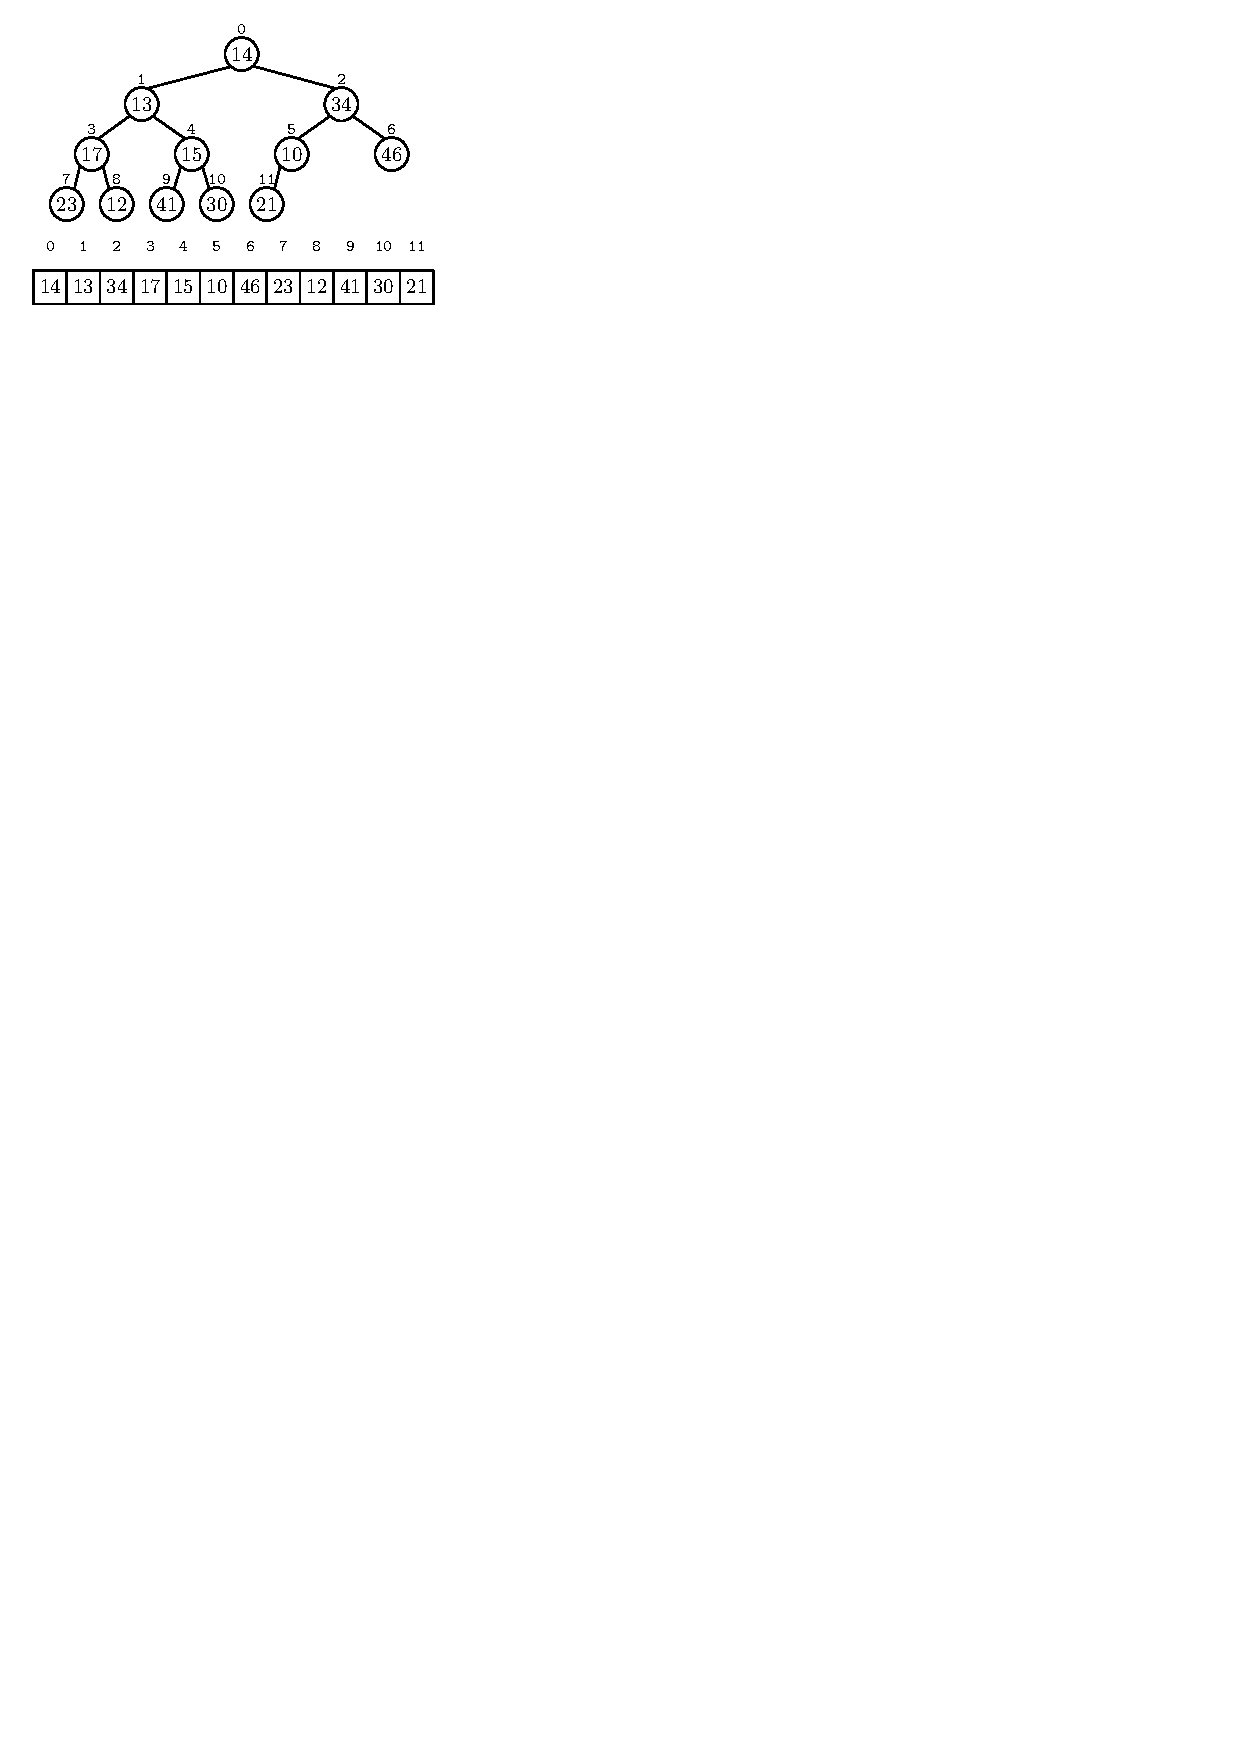
\includegraphics[width=0.9\textwidth]{img/img8.pdf}};
        \node<2> (i2) {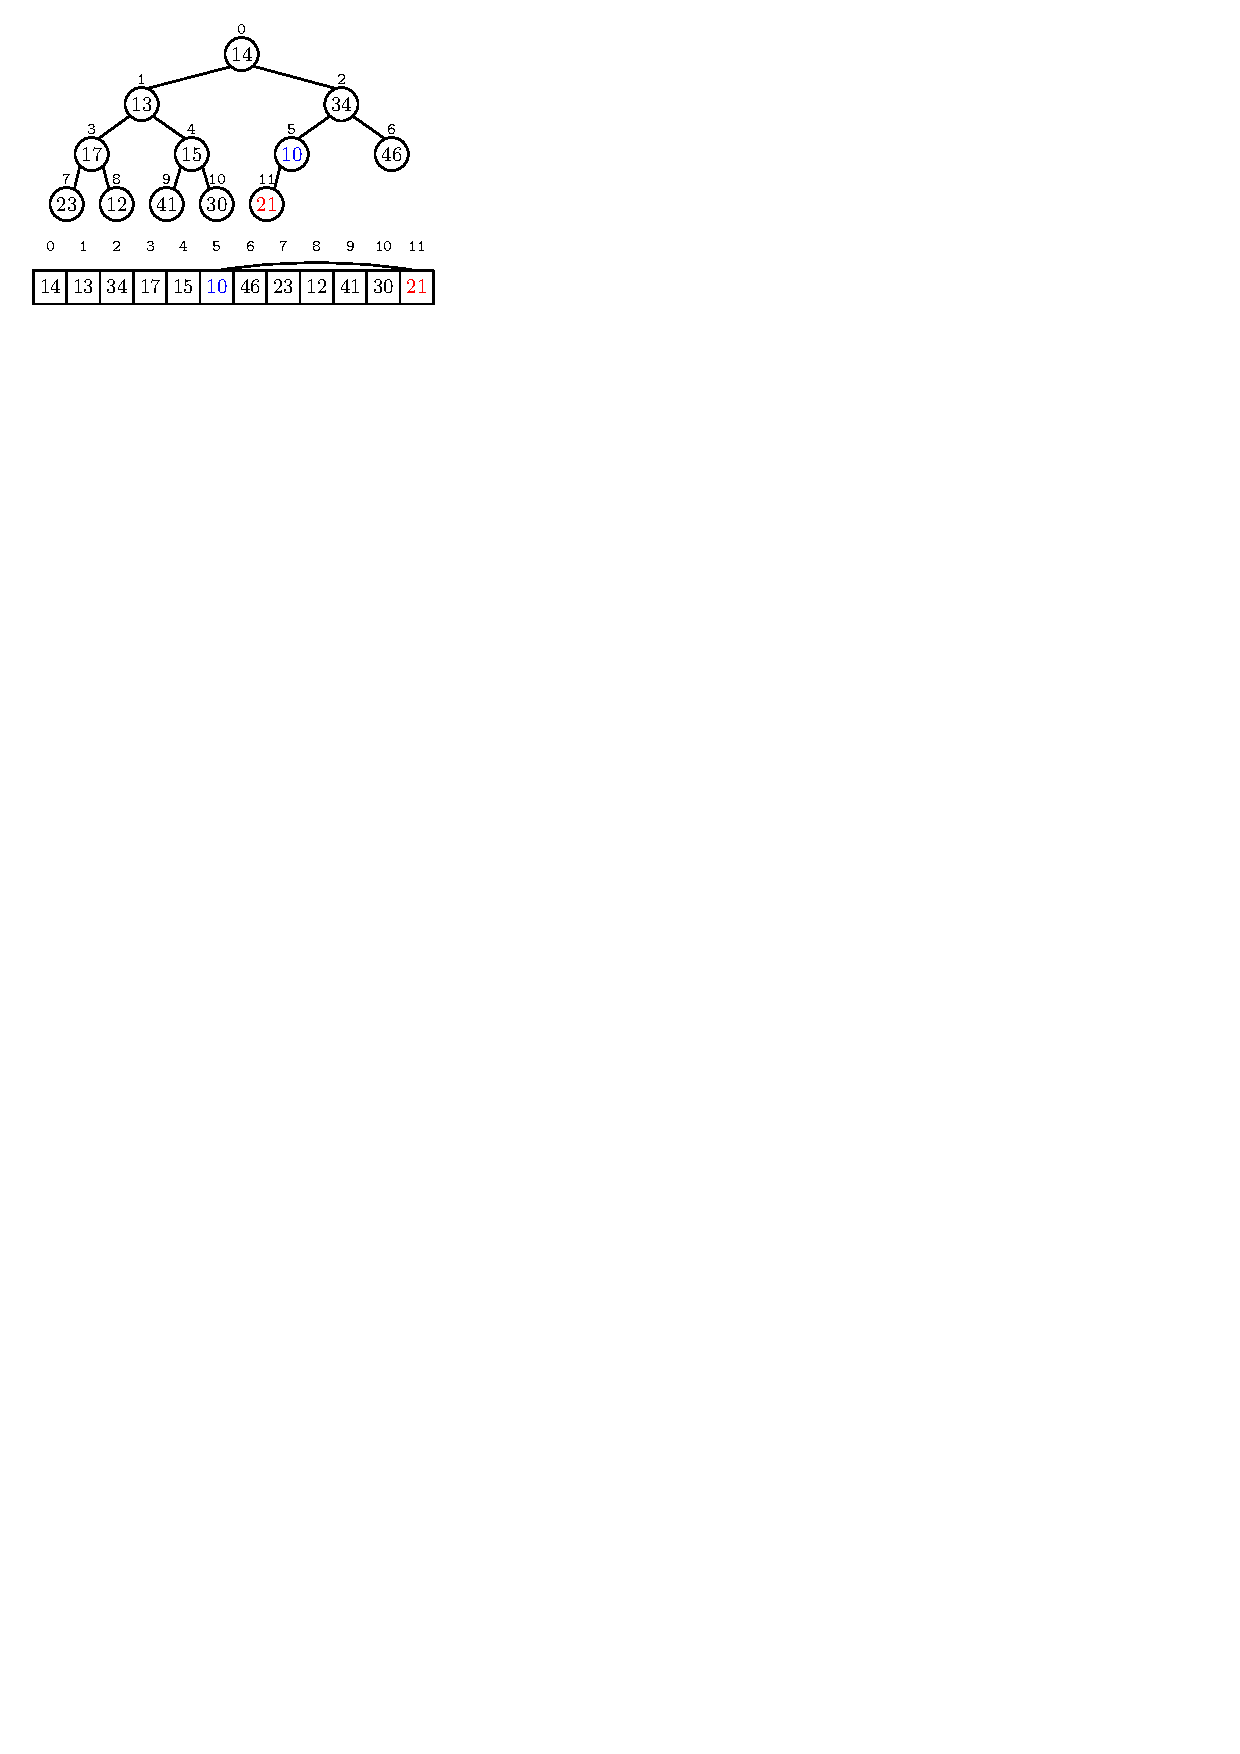
\includegraphics[width=0.9\textwidth]{img/img9.pdf}};
        \node<3> (i3) {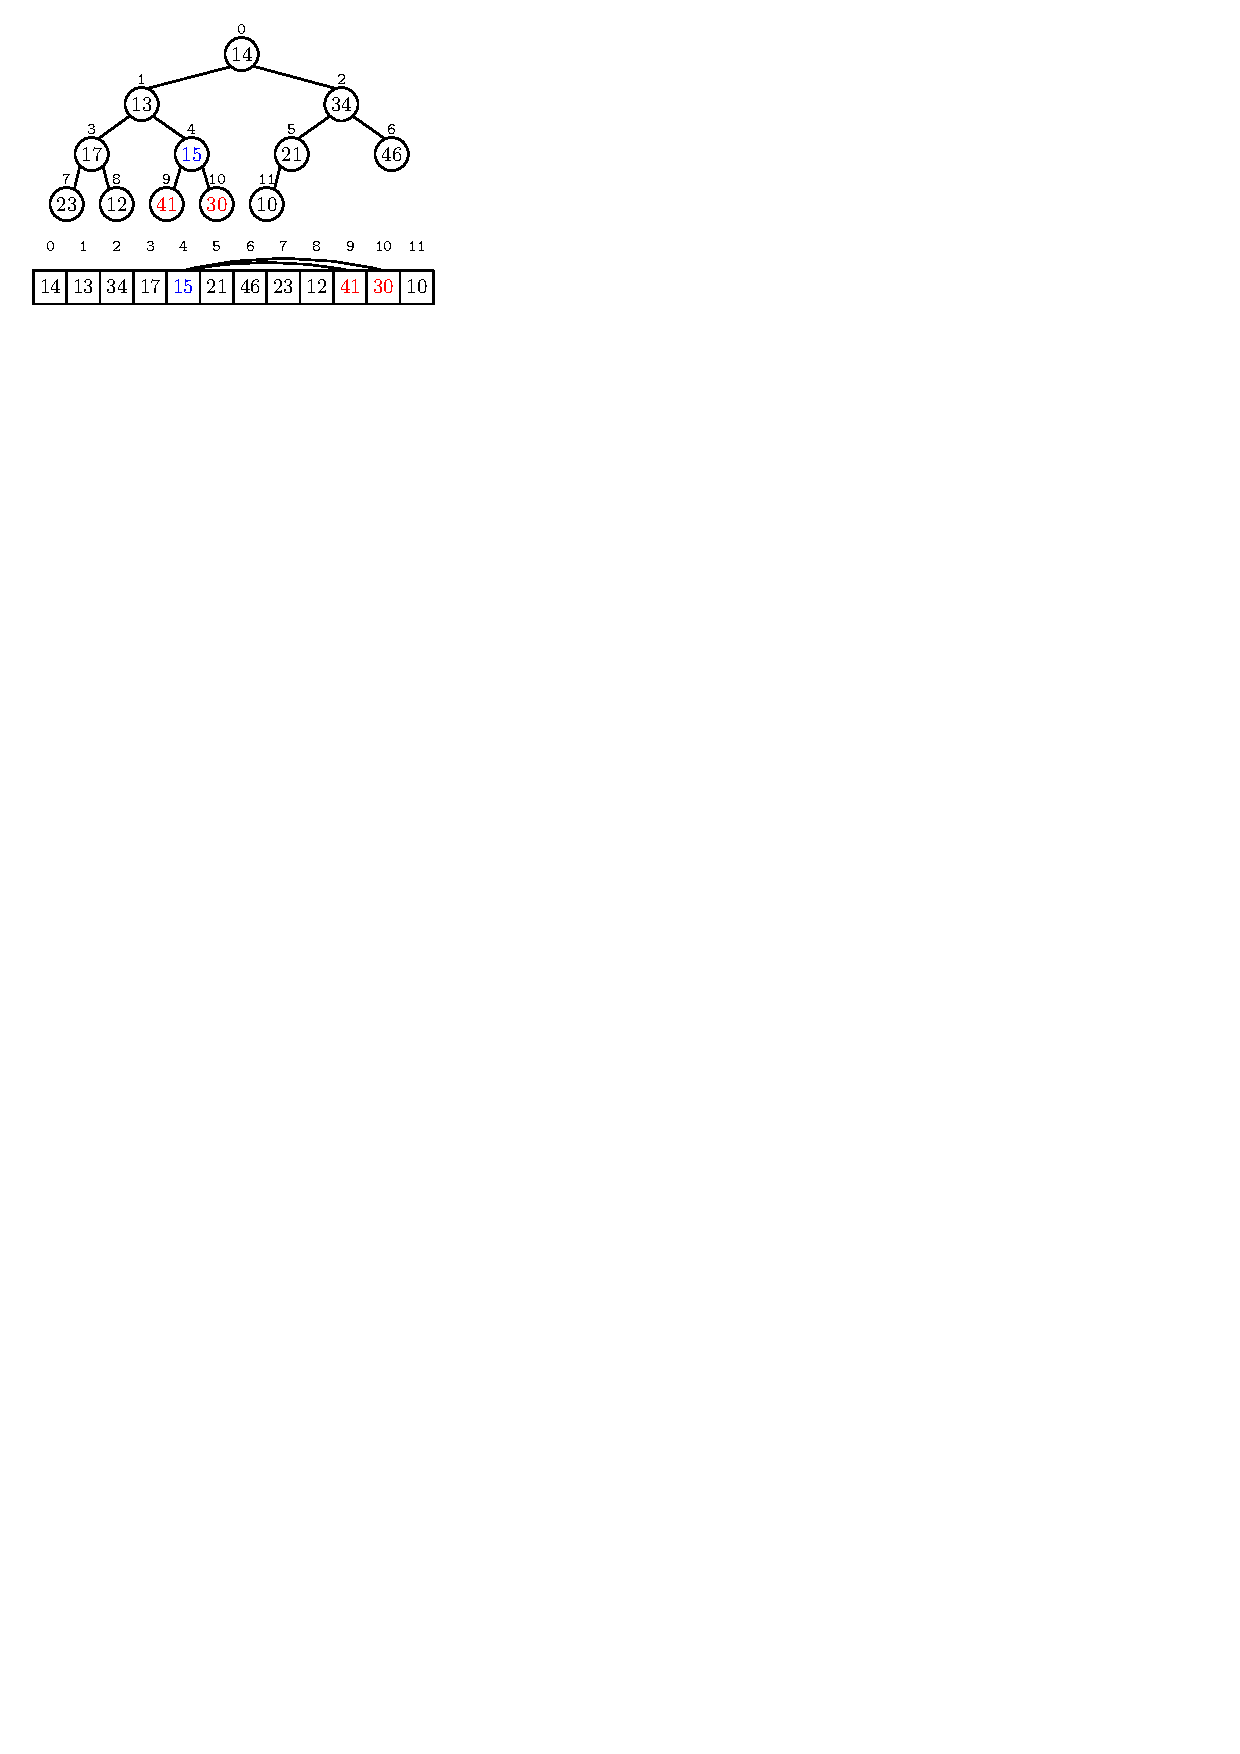
\includegraphics[width=0.9\textwidth]{img/img10.pdf}};
        \node<4> (i4) {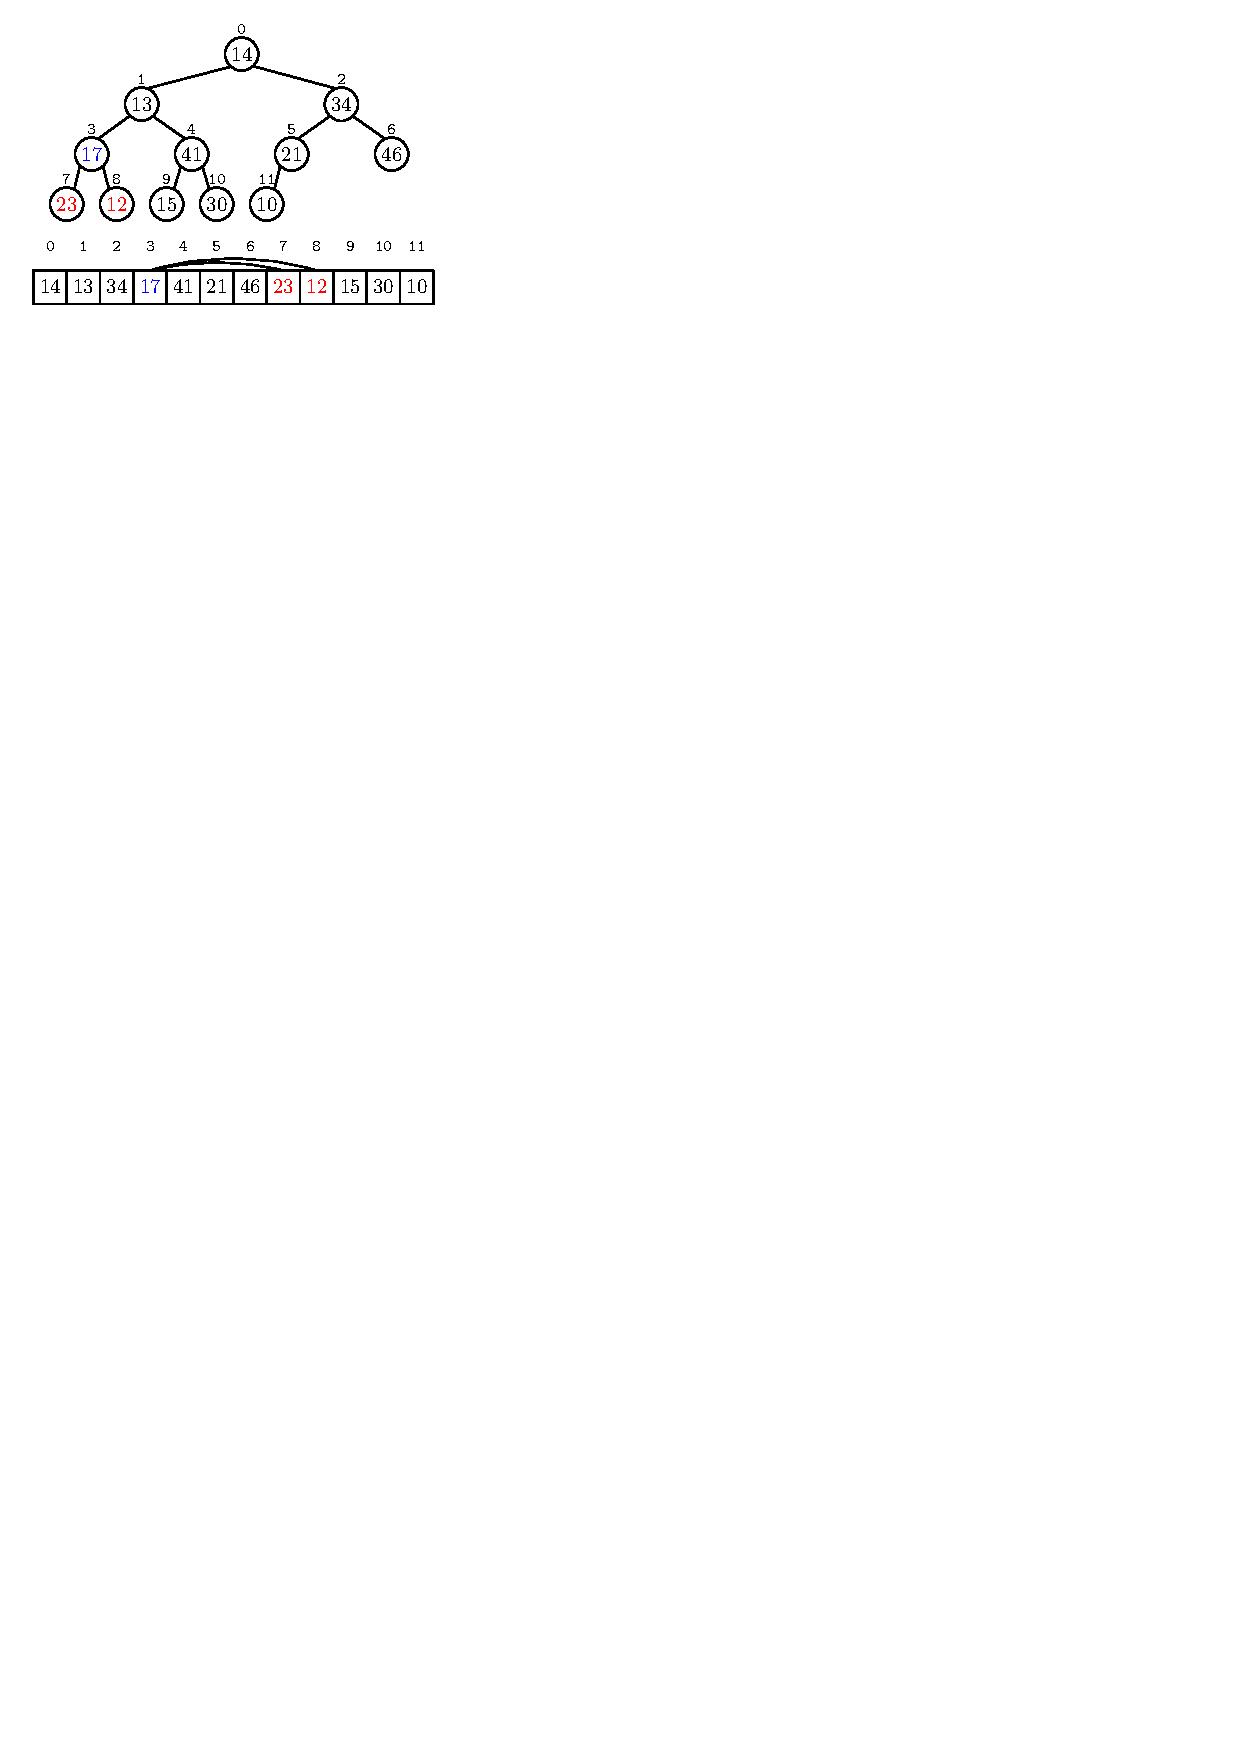
\includegraphics[width=0.9\textwidth]{img/img11.pdf}};
        \node<5> (i5) {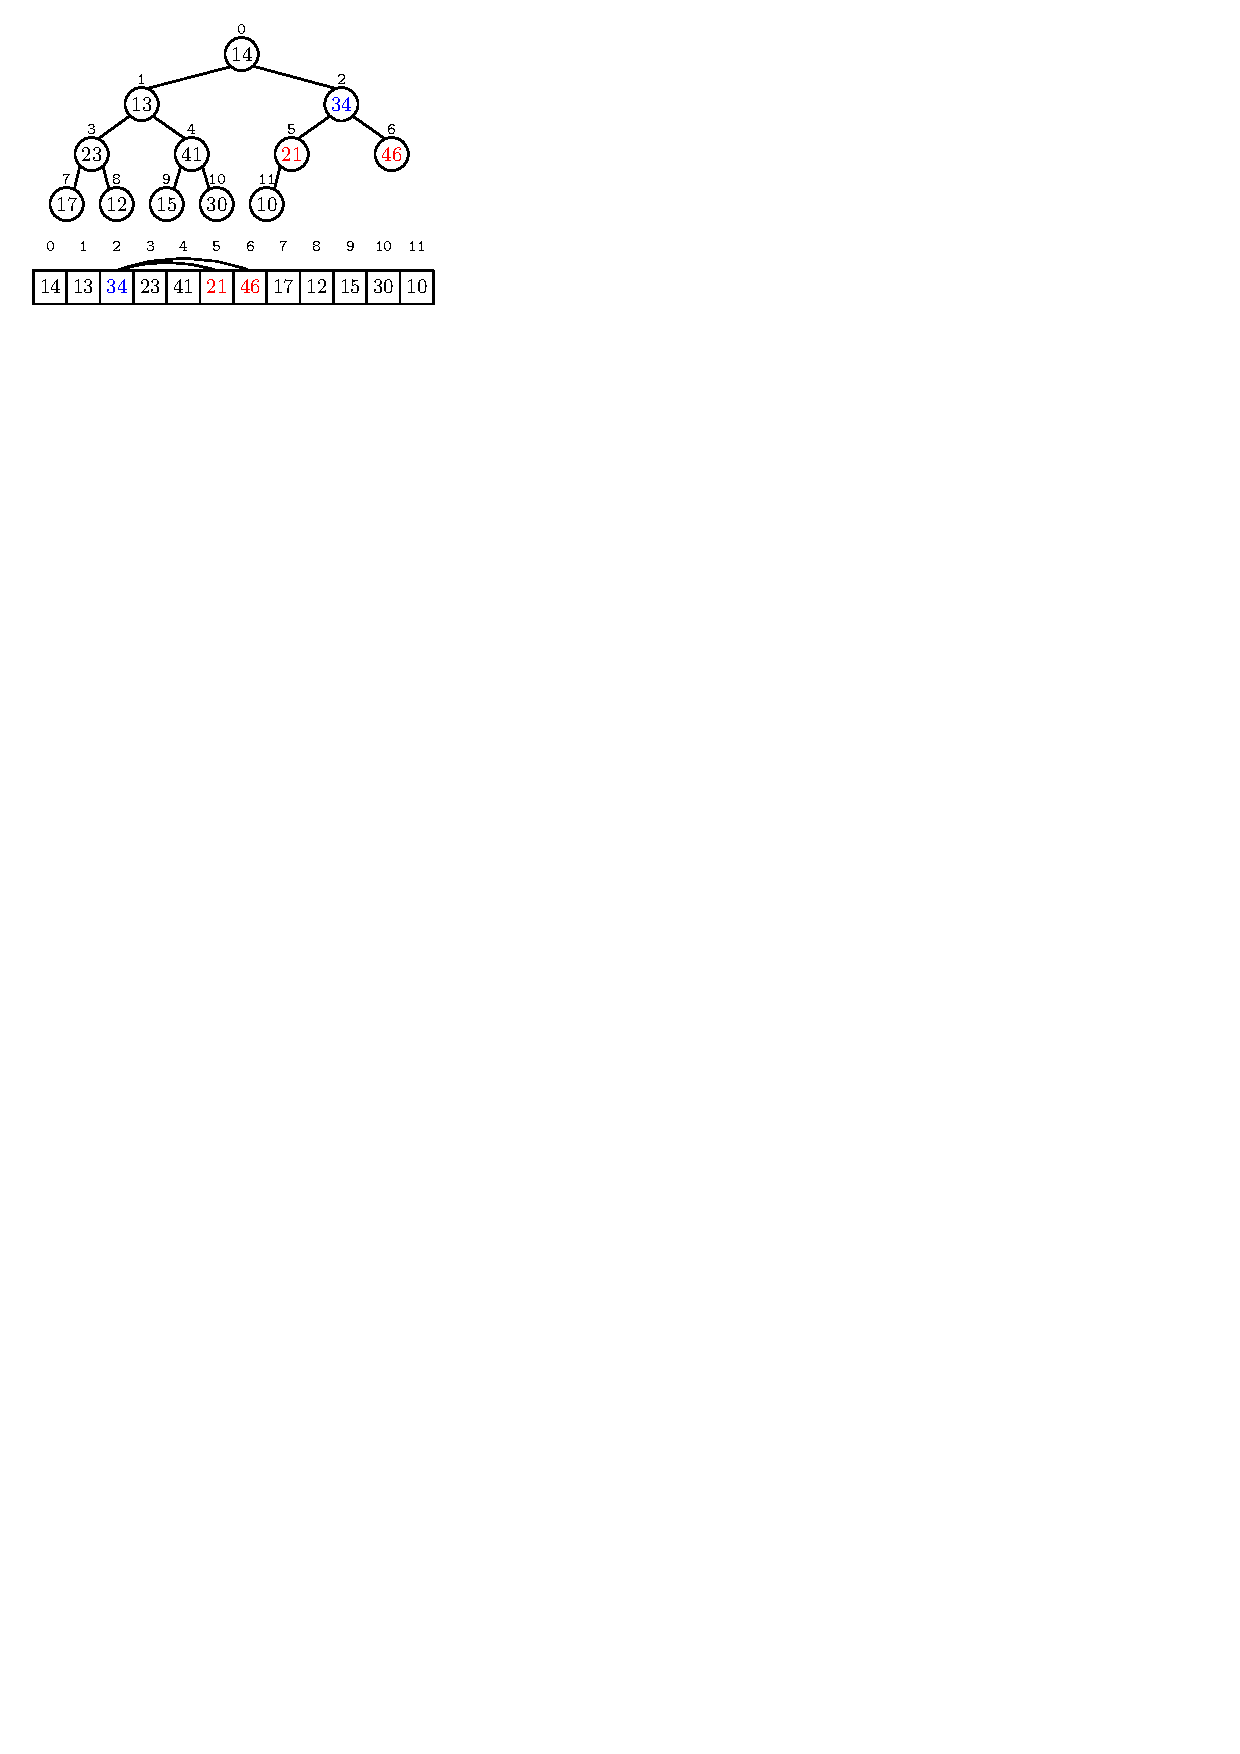
\includegraphics[width=0.9\textwidth]{img/img12.pdf}};
        \node<6> (i6) {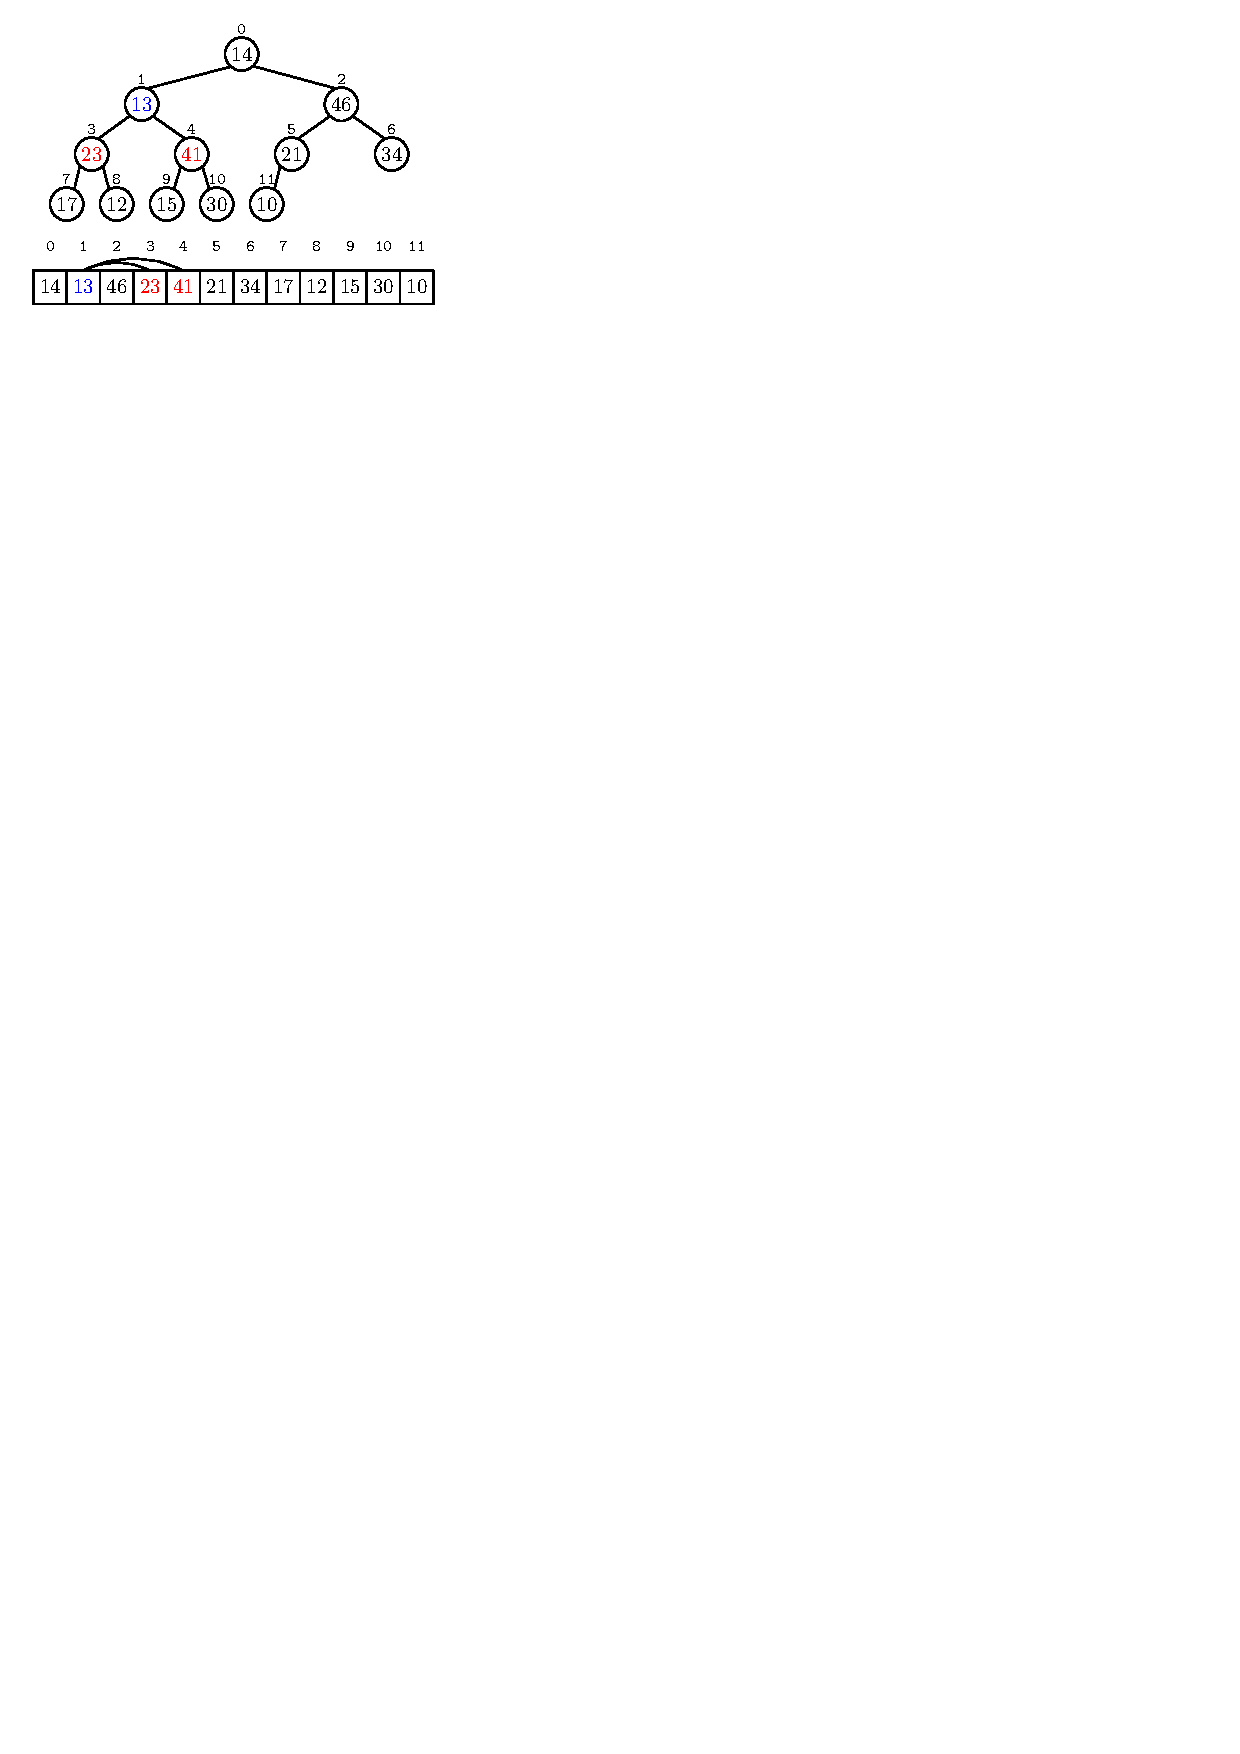
\includegraphics[width=0.9\textwidth]{img/img13.pdf}};
        \node<7> (i7) {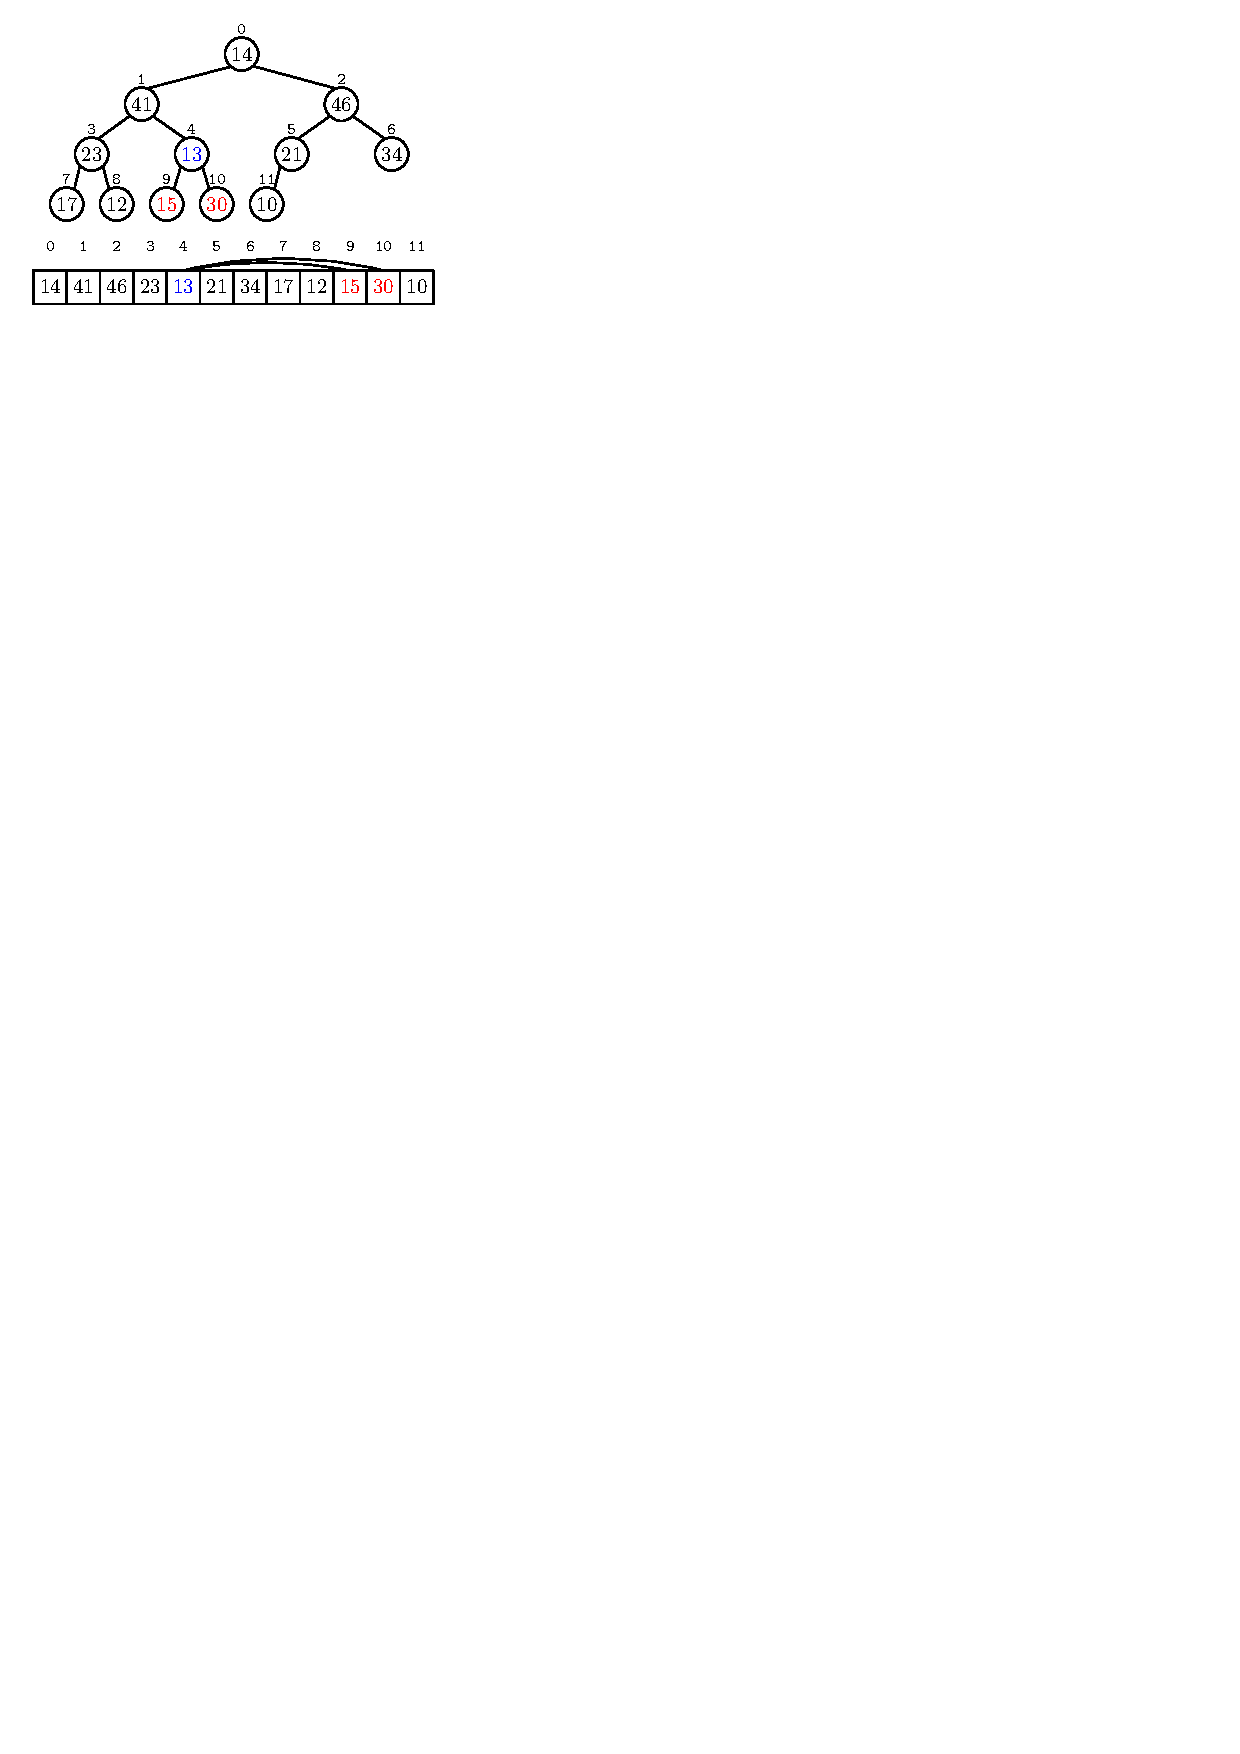
\includegraphics[width=0.9\textwidth]{img/img14.pdf}};
        \node<8> (i8) {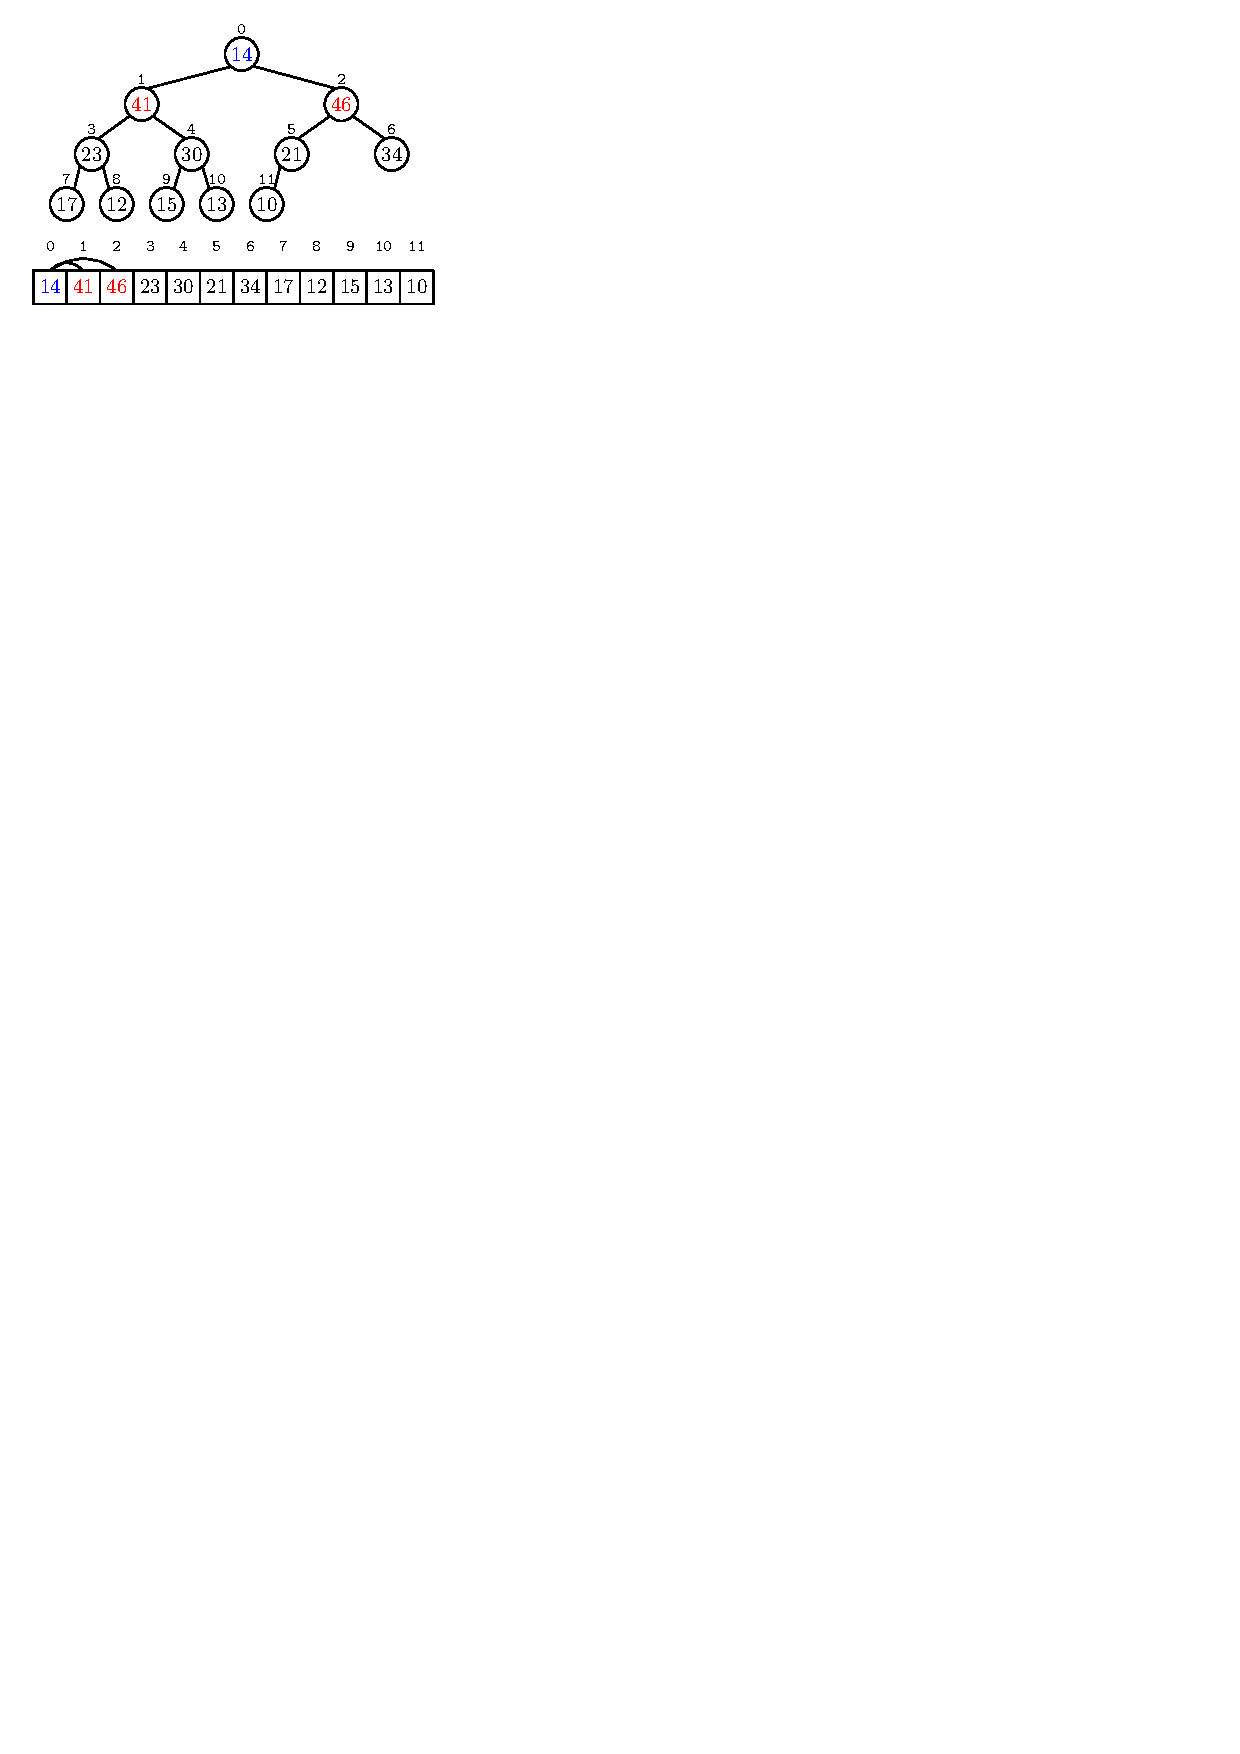
\includegraphics[width=0.9\textwidth]{img/img15.pdf}};
        \node<9> (i9) {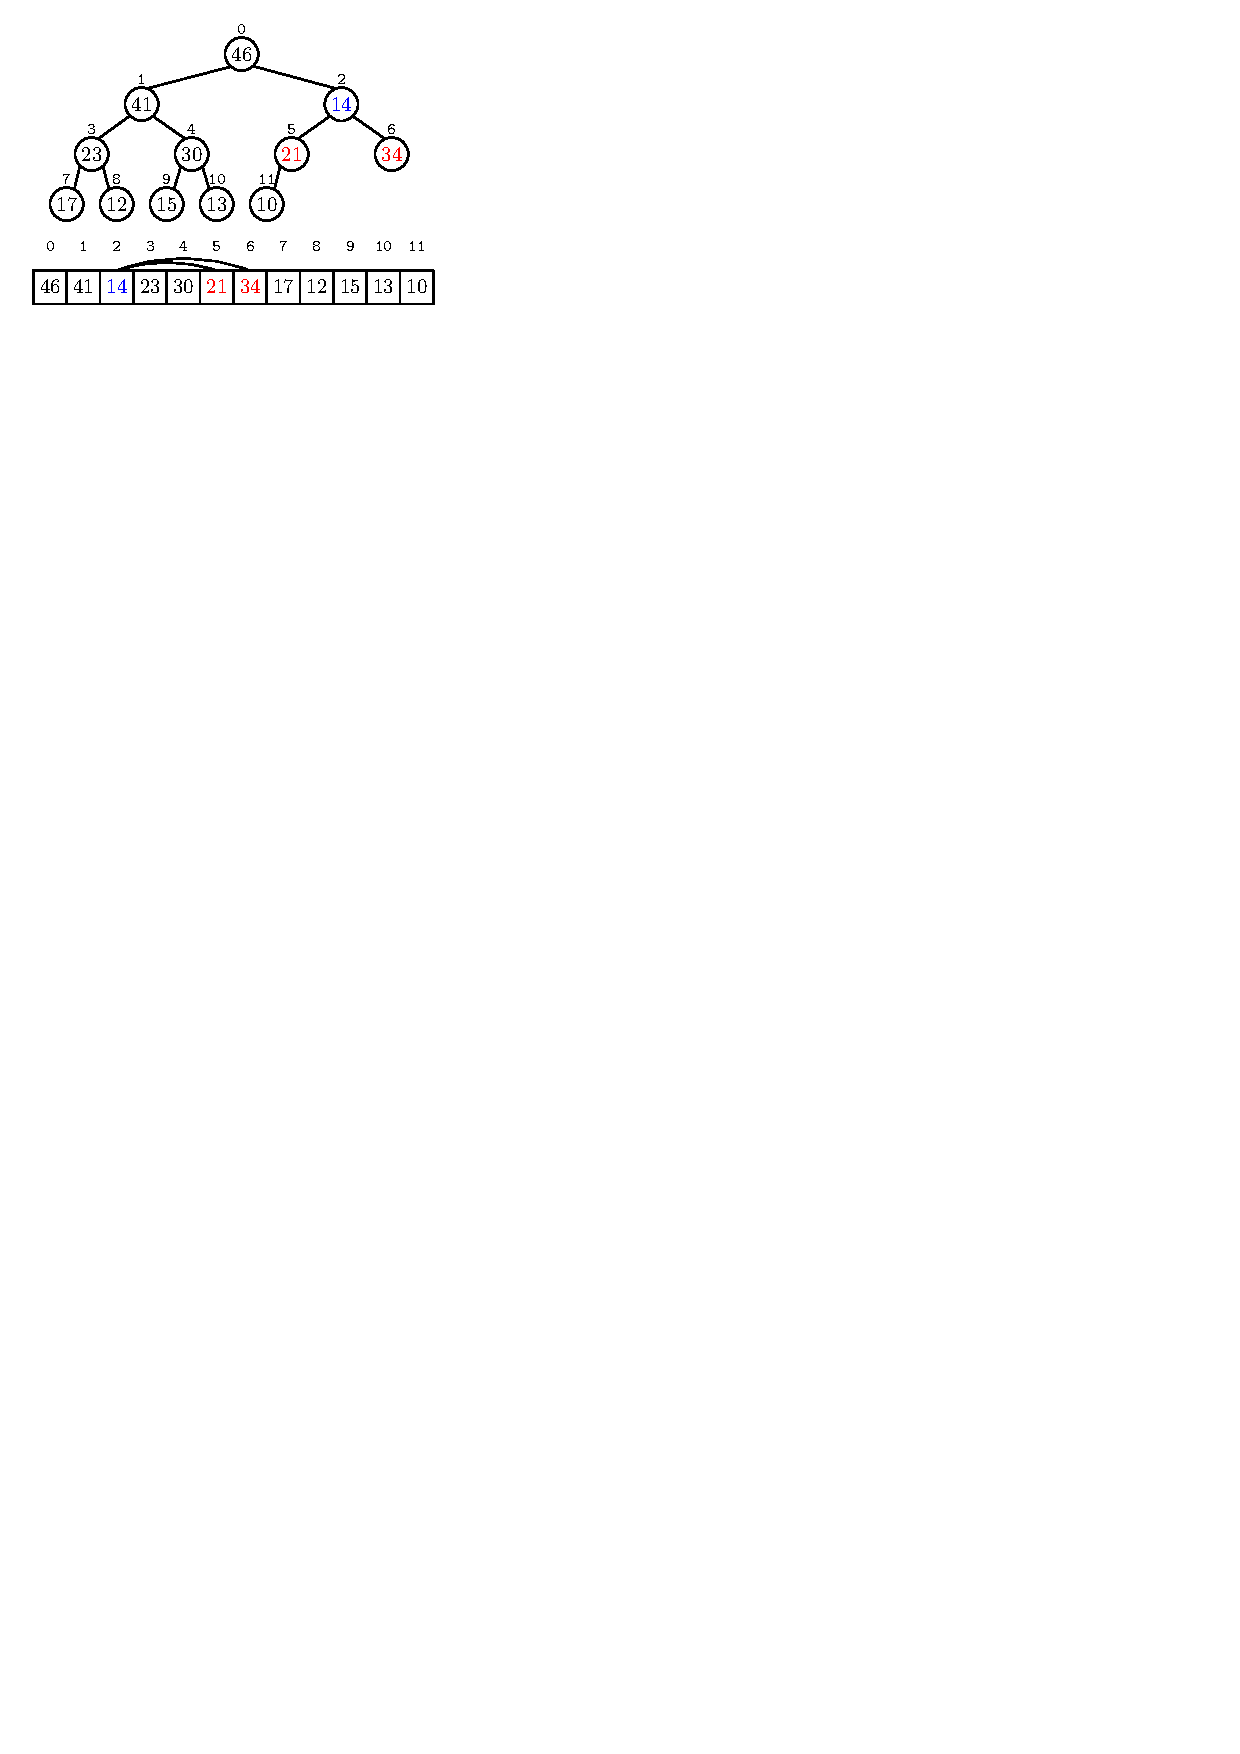
\includegraphics[width=0.9\textwidth]{img/img16.pdf}};
        \node<10> (i10) {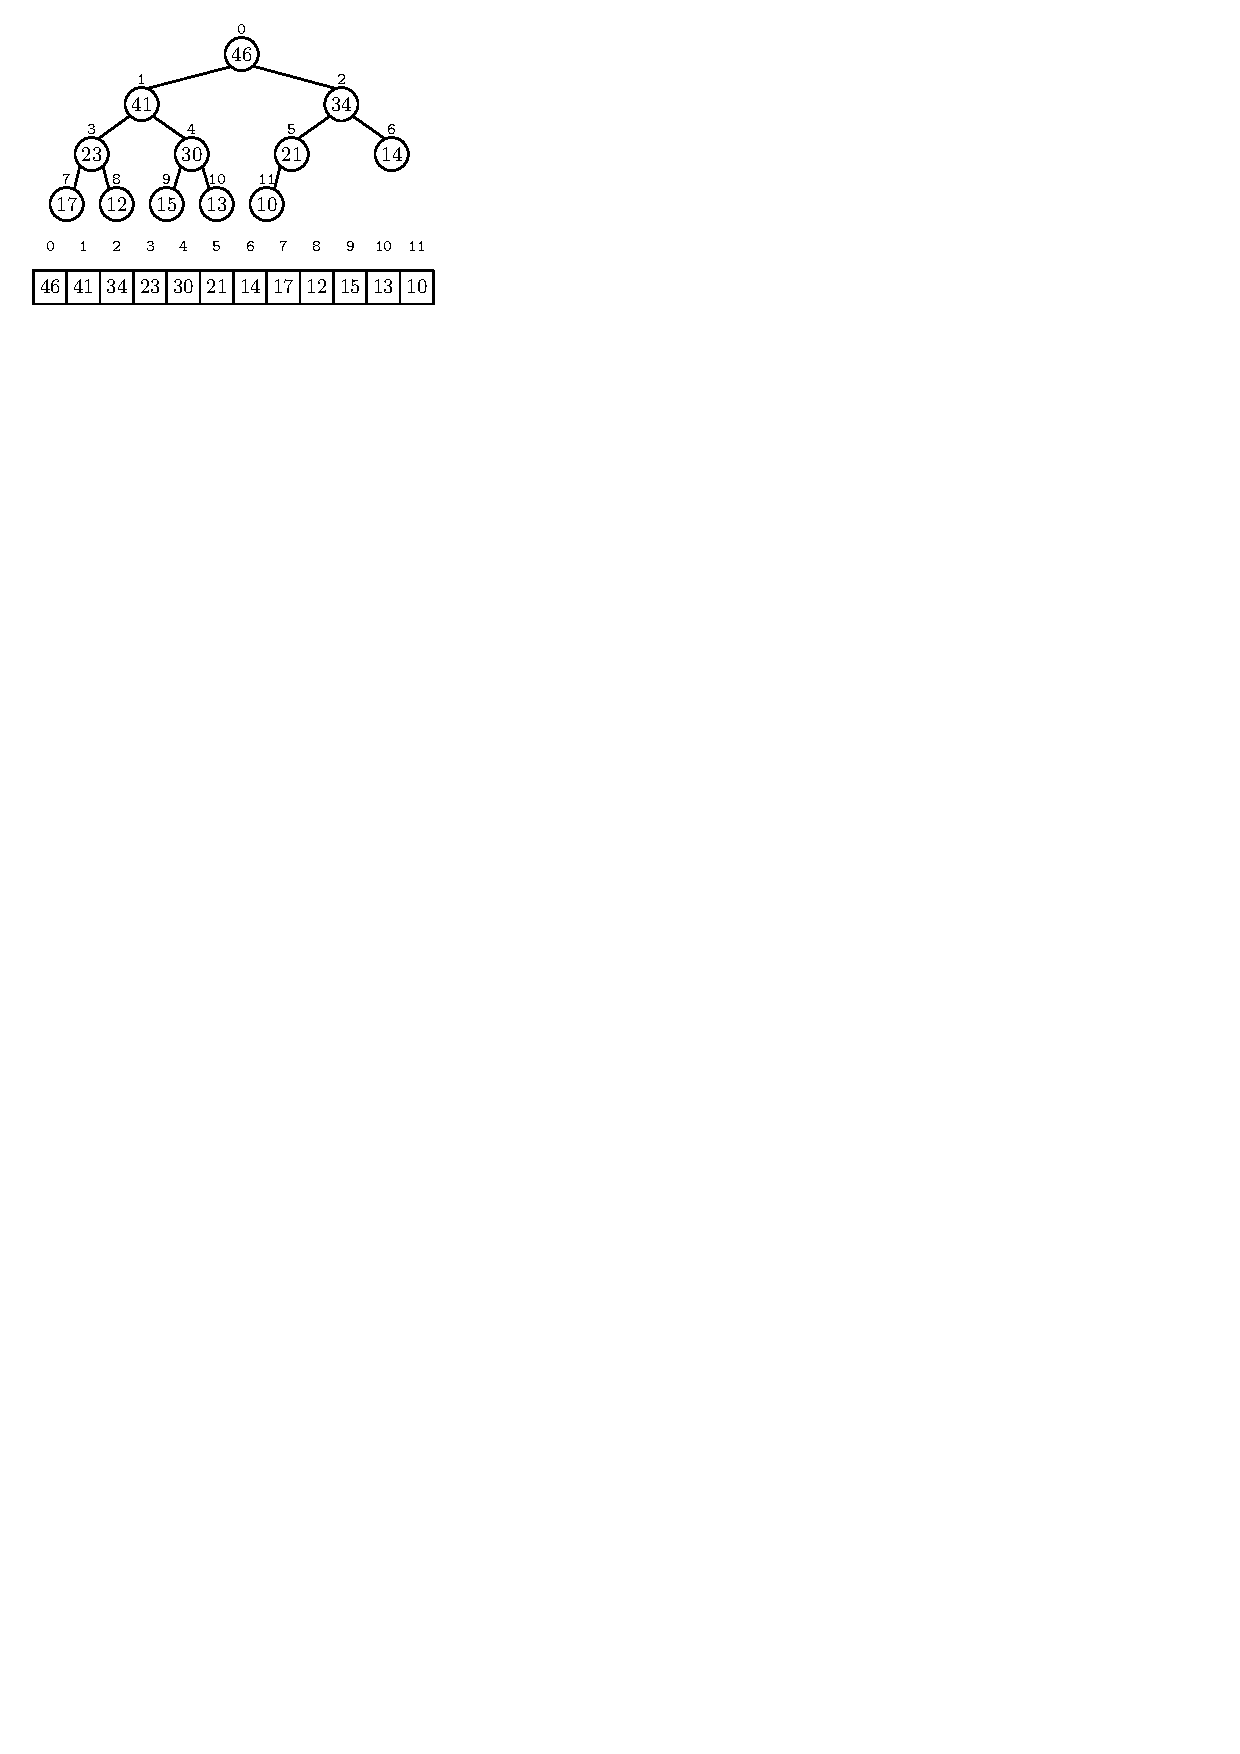
\includegraphics[width=0.9\textwidth]{img/img17.pdf}};
      \end{tikzpicture}
    \end{figure}
  \end{frame}

  \begin{frame}[fragile]{Construção de um \emph{heap} máximo - Implementação}
    %\vspace{-1em}
    \begin{center}
    \begin{minipage}{0.52\textwidth}
    \only<2>{\setminted{highlightlines=2}}
    \only<3>{\setminted{highlightlines=4}}
    \only<4>{\setminted{highlightlines=5}}
    \begin{minted}{c}
    void buildMaxHeap (int * v, int n) {
      int lp = lastParent(n), comp = 0;
      
      for (int i = lp; i >= 0; i--)
        comp += maxHeapify(v, n, i);
        
      return comp;
    }
    \end{minted}
    \end{minipage}
    \end{center}
    
    %\vspace{1em}
    
    \pause
    Análise grosseira do custo:
    
    \begin{itemize}
      \item<2-> Linha 2 tem custo $O(1)$;
      \item<3-> Linha 4 tem custo $O\left(\left\lfloor\frac{n}{2}\right\rfloor - 1\right) = O(n)$;
      \item<4-> Linha 5 tem custo $O(\log(n))$ como descrito anteriormente.
    \end{itemize}

    \begin{onlyenv}<5>
      Isso totaliza, então, $O(n\log(n))$.
      
      No entanto, pode-se fazer uma análise mais refinada. \textbf{Como?}
    \end{onlyenv}
  \end{frame}

  \begin{frame}[fragile]{Construção de um \emph{heap} máximo - Análise refinada}
    Dado um \emph{heap} \texttt{v[0..n - 1]}:
    
    \begin{itemize}
      \item Sua altura $h$ é $\lfloor\log(n)\rfloor$;
      \item O máximo de nós em uma altura $h$ é $\left\lceil\frac{n}{2^{h + 1}}\right\rceil$.
    \end{itemize}
    
    Então pode-se expressar o custo de \texttt{maxHeapify} por $O(h)$.
    
    \vspace{1em}
    \begin{center}
      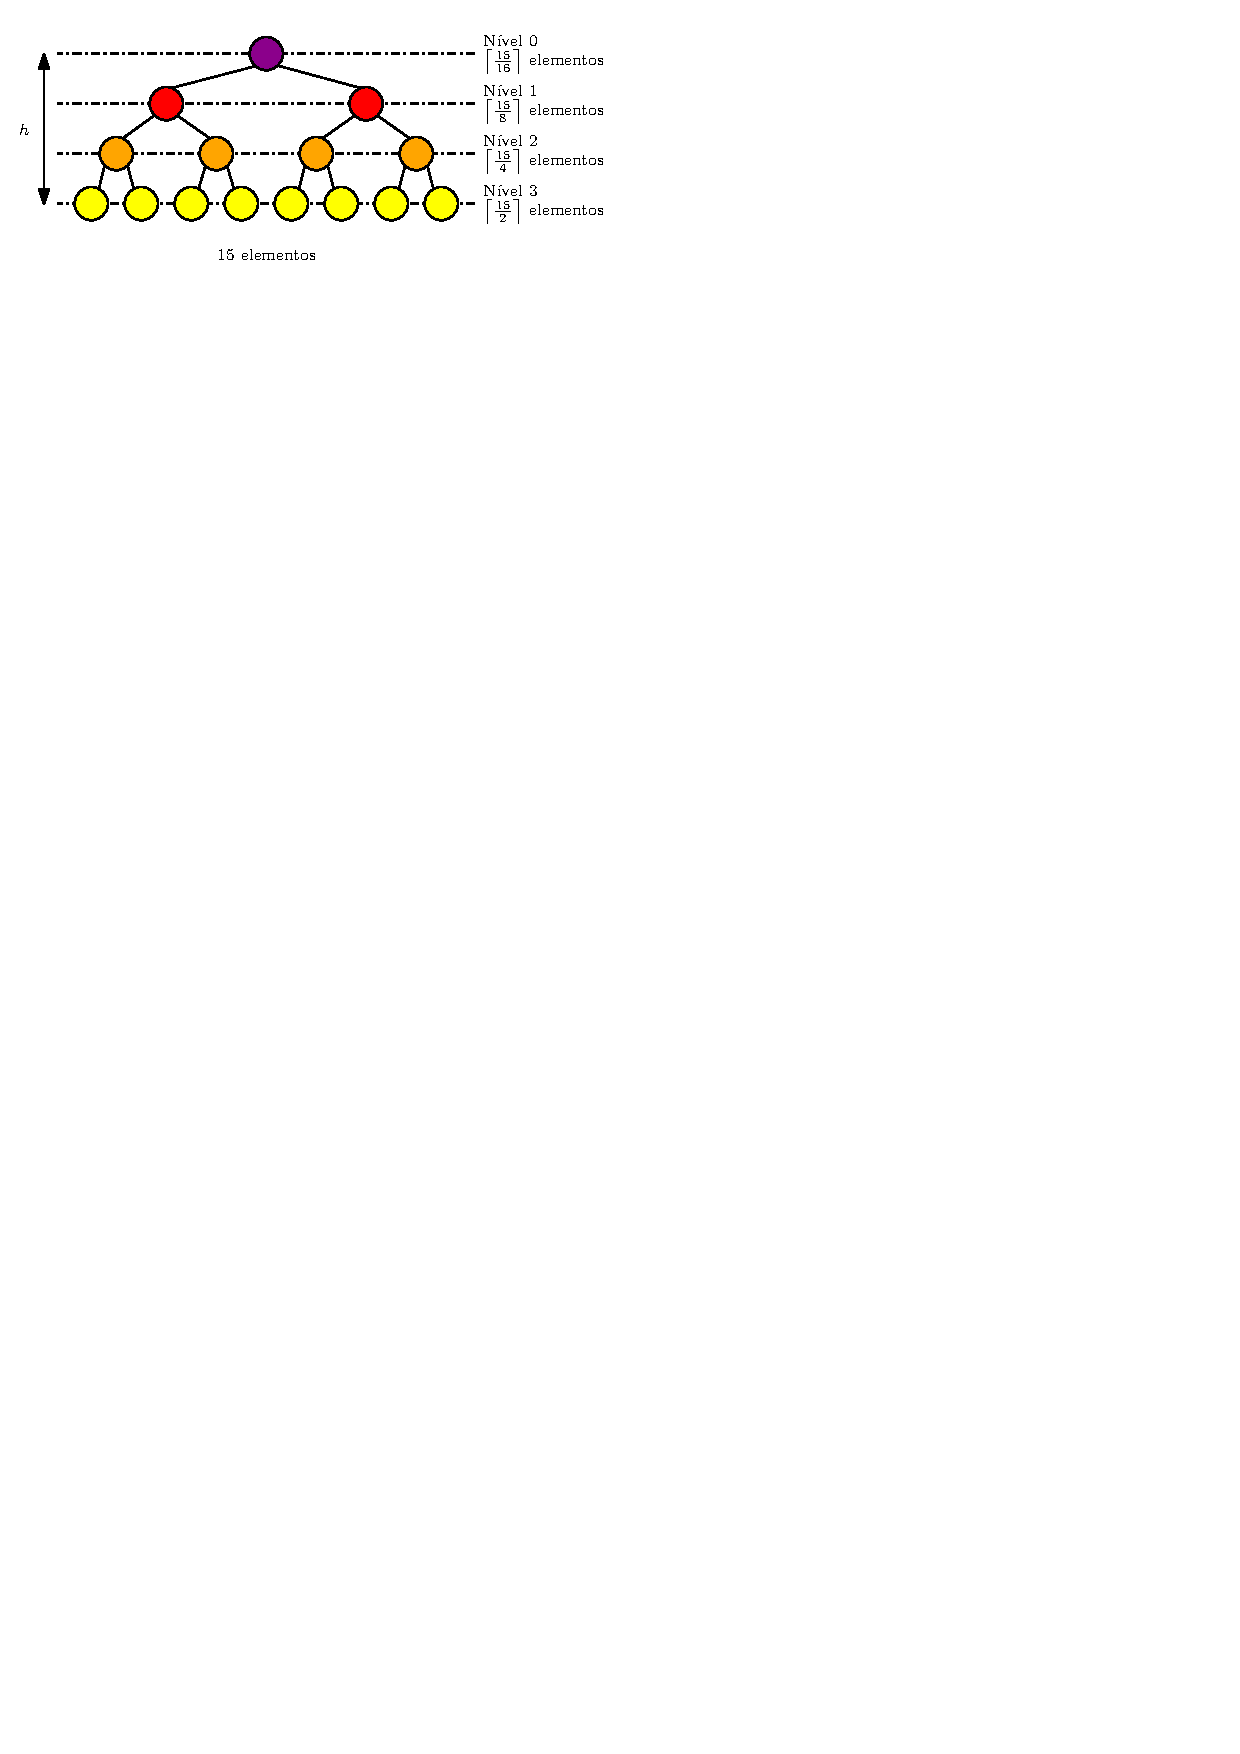
\includegraphics[width=\textwidth]{img/img19.pdf}
    \end{center}   
  \end{frame}

  \begin{frame}{Construção de um \emph{heap} máximo - Análise refinada}
    O total de passos $N$ para construir um \emph{heap} de tamanho $n$
    pode ser escrito matematicamente.

    Na altura $h$, existem $\frac{n}{2 ^ {h + 1}}$ elementos em que o
    \texttt{maxHeapify} precisa ser chamado, e sabemos que o 
    \texttt{maxHeapify} em uma altura $h$ tem custo no caso pior
    de $O(h)$. Então:
    
    \vspace{-1em}
    \begin{align*}
      N &= \sum_{h = 0}^{\lfloor\log(n)\rfloor} \frac{n}{2 ^ {h + 1}} \cdot h \\
        &= \frac{n}{2} \left(\sum_{h = 0}^{\lfloor\log(n)\rfloor} \frac{h}{2 ^ h}\right) \\
        &\leq \frac{n}{2} \left(\sum_{h = 0}^{\infty} \frac{h}{2 ^ h}\right)
    \end{align*}
    
  \end{frame}

  \begin{frame}{Construção de um \emph{heap} máximo - Análise refinada}
    A solução do último somatório pode ser achada derivando ambos os lados
    da equação da série geométrica \footnotemark[1]:

    \begin{align*}
      \frac{\partial}{\partial x}\left(\sum_{k = 0}^{\infty} x ^ k\right)
      &= \frac{\partial}{\partial x}\left(\frac{1}{1 - x}\right) \\
      \sum_{k = 0}^{\infty} kx ^ k &= \frac{x}{(1 - x) ^ 2}
    \end{align*}

    \footnotetext[1]{Para mais detalhes sobre, consultar o Cormen, apêndice A.8. }
  \end{frame}

  \begin{frame}[c]{Construção de um \emph{heap} máximo - Análise refinada}
    Então, substituindo $x = \frac{1}{2}$ na equação superior:

    \begin{align*}
      \sum_{k = 0}^{\infty} k \cdot \left(\frac{1}{2}\right) ^ k =
      \frac{(1 / 2)}{(1 - 1 / 2) ^ 2} = 2
    \end{align*}

    Substituindo a solução do somatório de volta:

    $$N \leq \frac{\cancel{2}n}{\cancel{2}} = n$$

    Assim, o custo de \texttt{buildMaxHeap} no pior caso é $O(n)$ \footnotemark[1].

    \footnotetext[1]{Tópico no StackOverflow: \url{https://bit.ly/2HW0yCJ}}
  \end{frame}

  \section{Heapsort}
  \begin{frame}{Heap Sort}
    \begin{itemize}
      \item Permite ordenar um vetor em ordem crescente ou decrescente;
      \item Realiza muitas trocas entre os elementos;
      \item Não é necessário um vetor auxiliar como no Merge Sort;
      \item Não precisa escolher um ótimo pivô como no Quick Sort.
    \end{itemize}
  \end{frame}

  \begin{frame}[c]{Heap Sort}
    \setbeamercolor{math text}{fg=black}
    \begin{center}
    \begin{minipage}{0.61\textwidth}
    \begin{algorithm}[H]
      \caption{$\textsc{Heapsort}(v,n)$}
      $\textsc{Build-Max-Heap}(v,n)$ \\
      \Para{$i \leftarrow n - 1$ \KwDownto \KwTo $1$}{
        $v[0] \leftrightarrow v[i]$ \\
        $\textsc{Max-Heapify}(v,i,0)$
      }
    \end{algorithm}
    \end{minipage}
    \end{center}
  \end{frame}

  \begin{frame}{Heap Sort - Exemplo}
    \begin{figure}[h!]
      \begin{tikzpicture}
        \node<1> (i1) {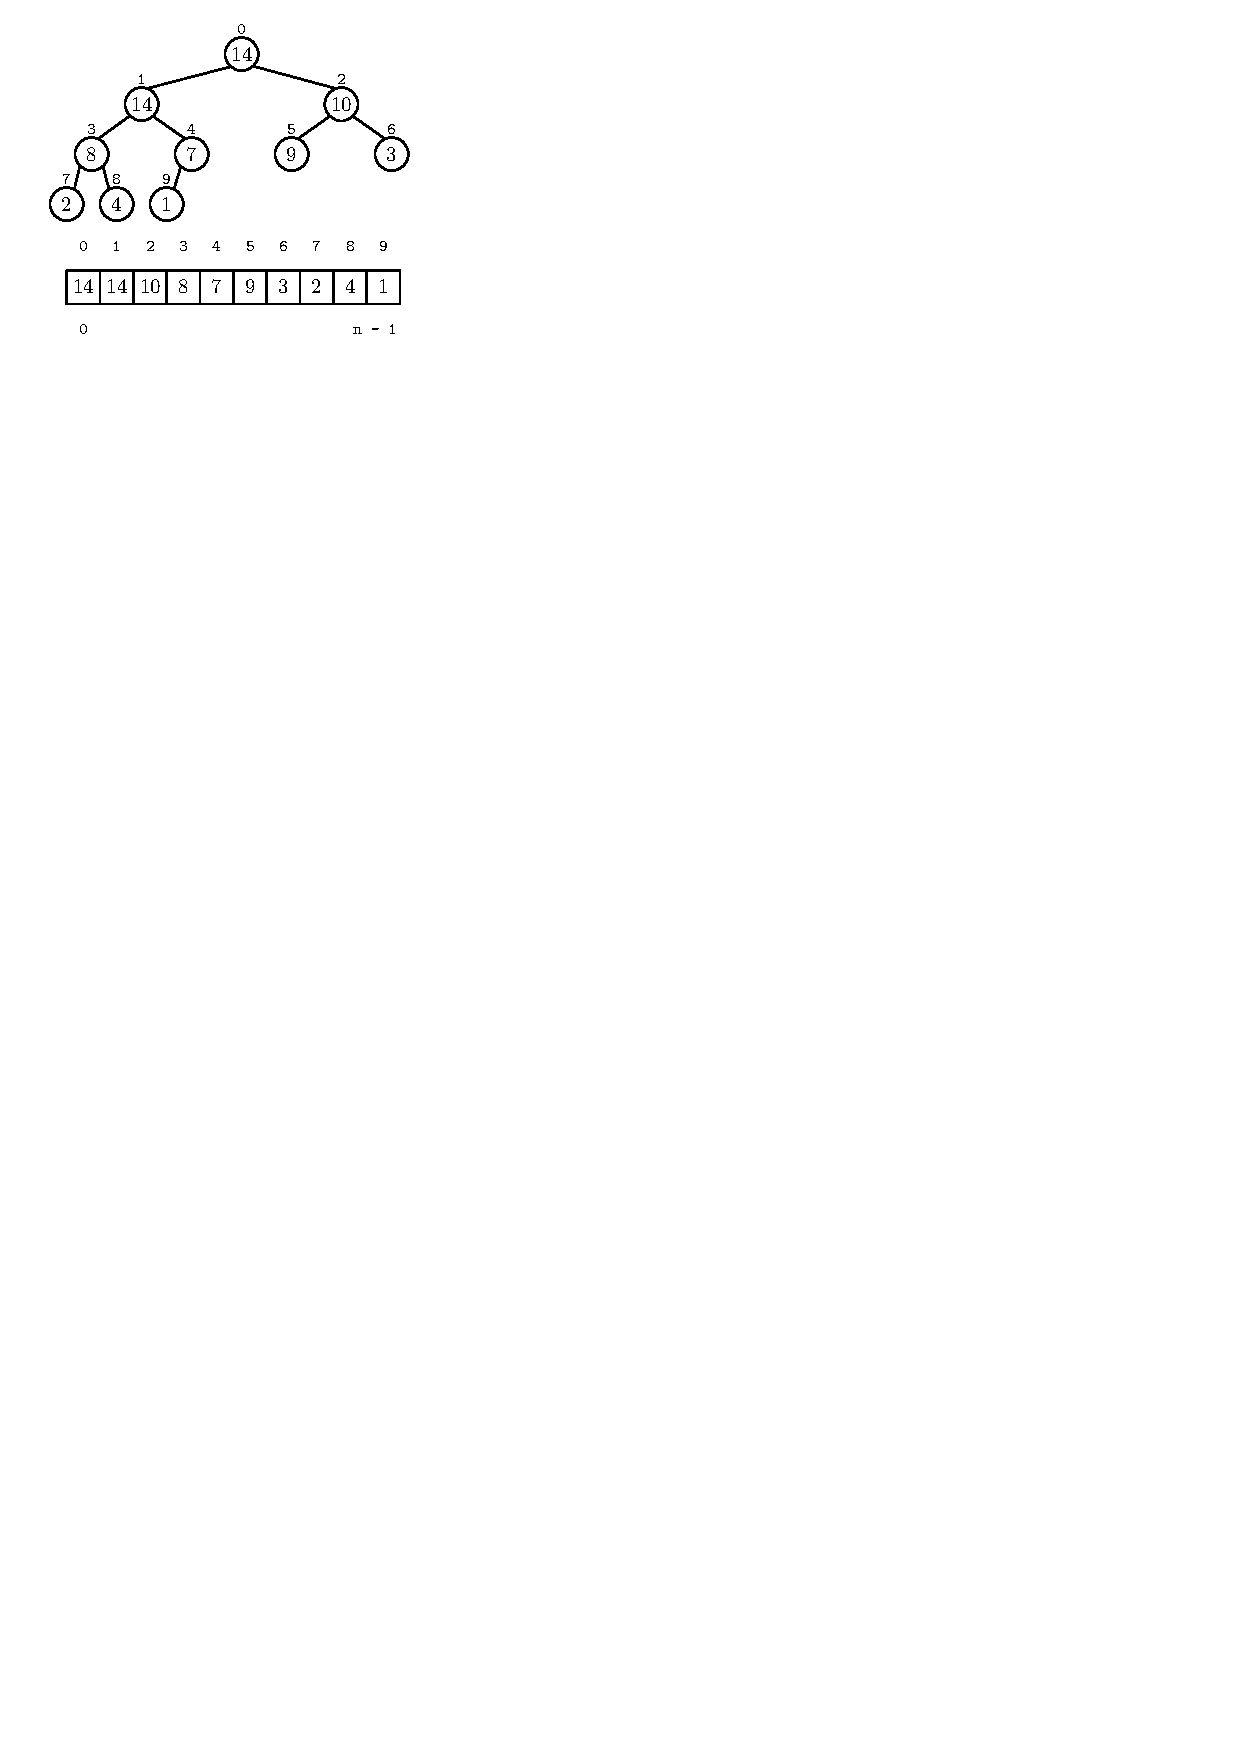
\includegraphics[width=0.8\textwidth]{img/img20.pdf}};
        \node<2> (i2) {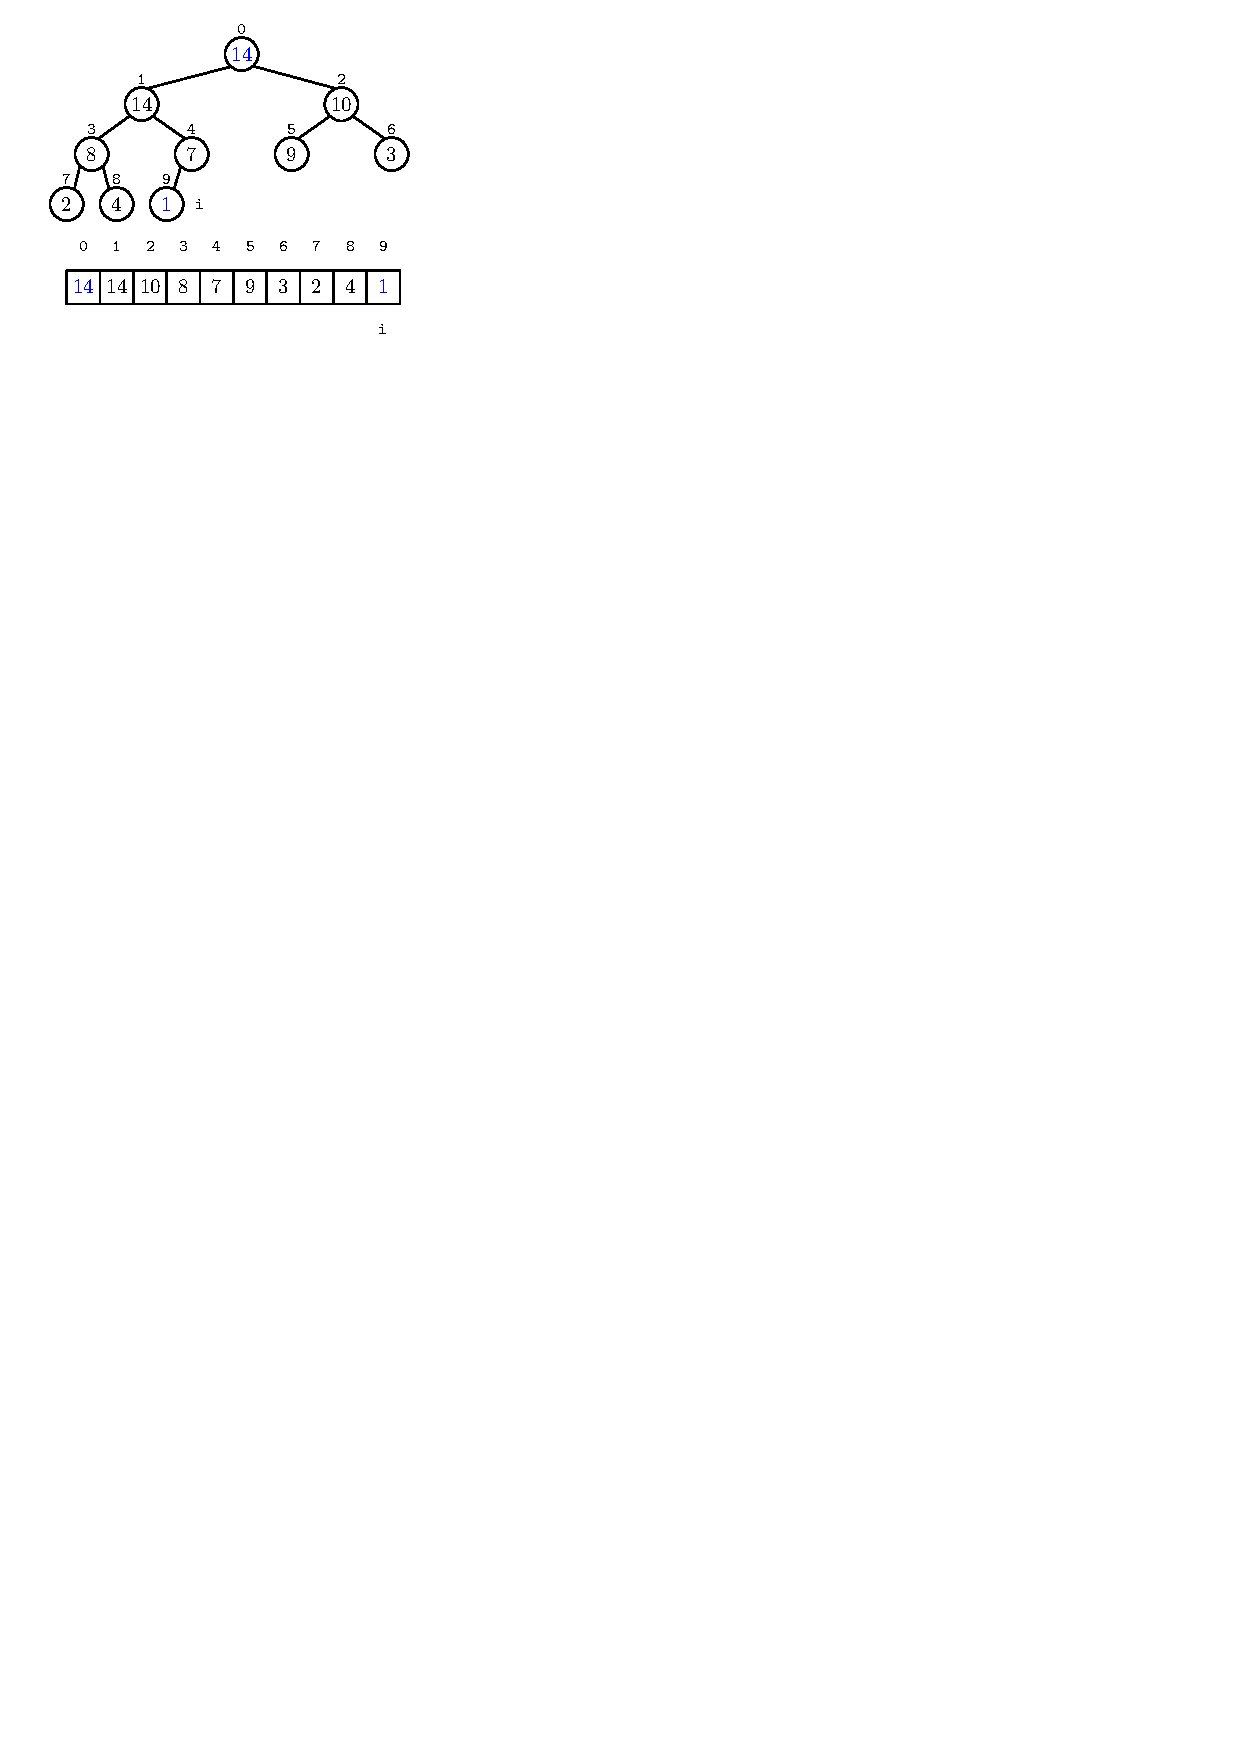
\includegraphics[width=0.8\textwidth]{img/img21.pdf}};
        \node<3> (i3) {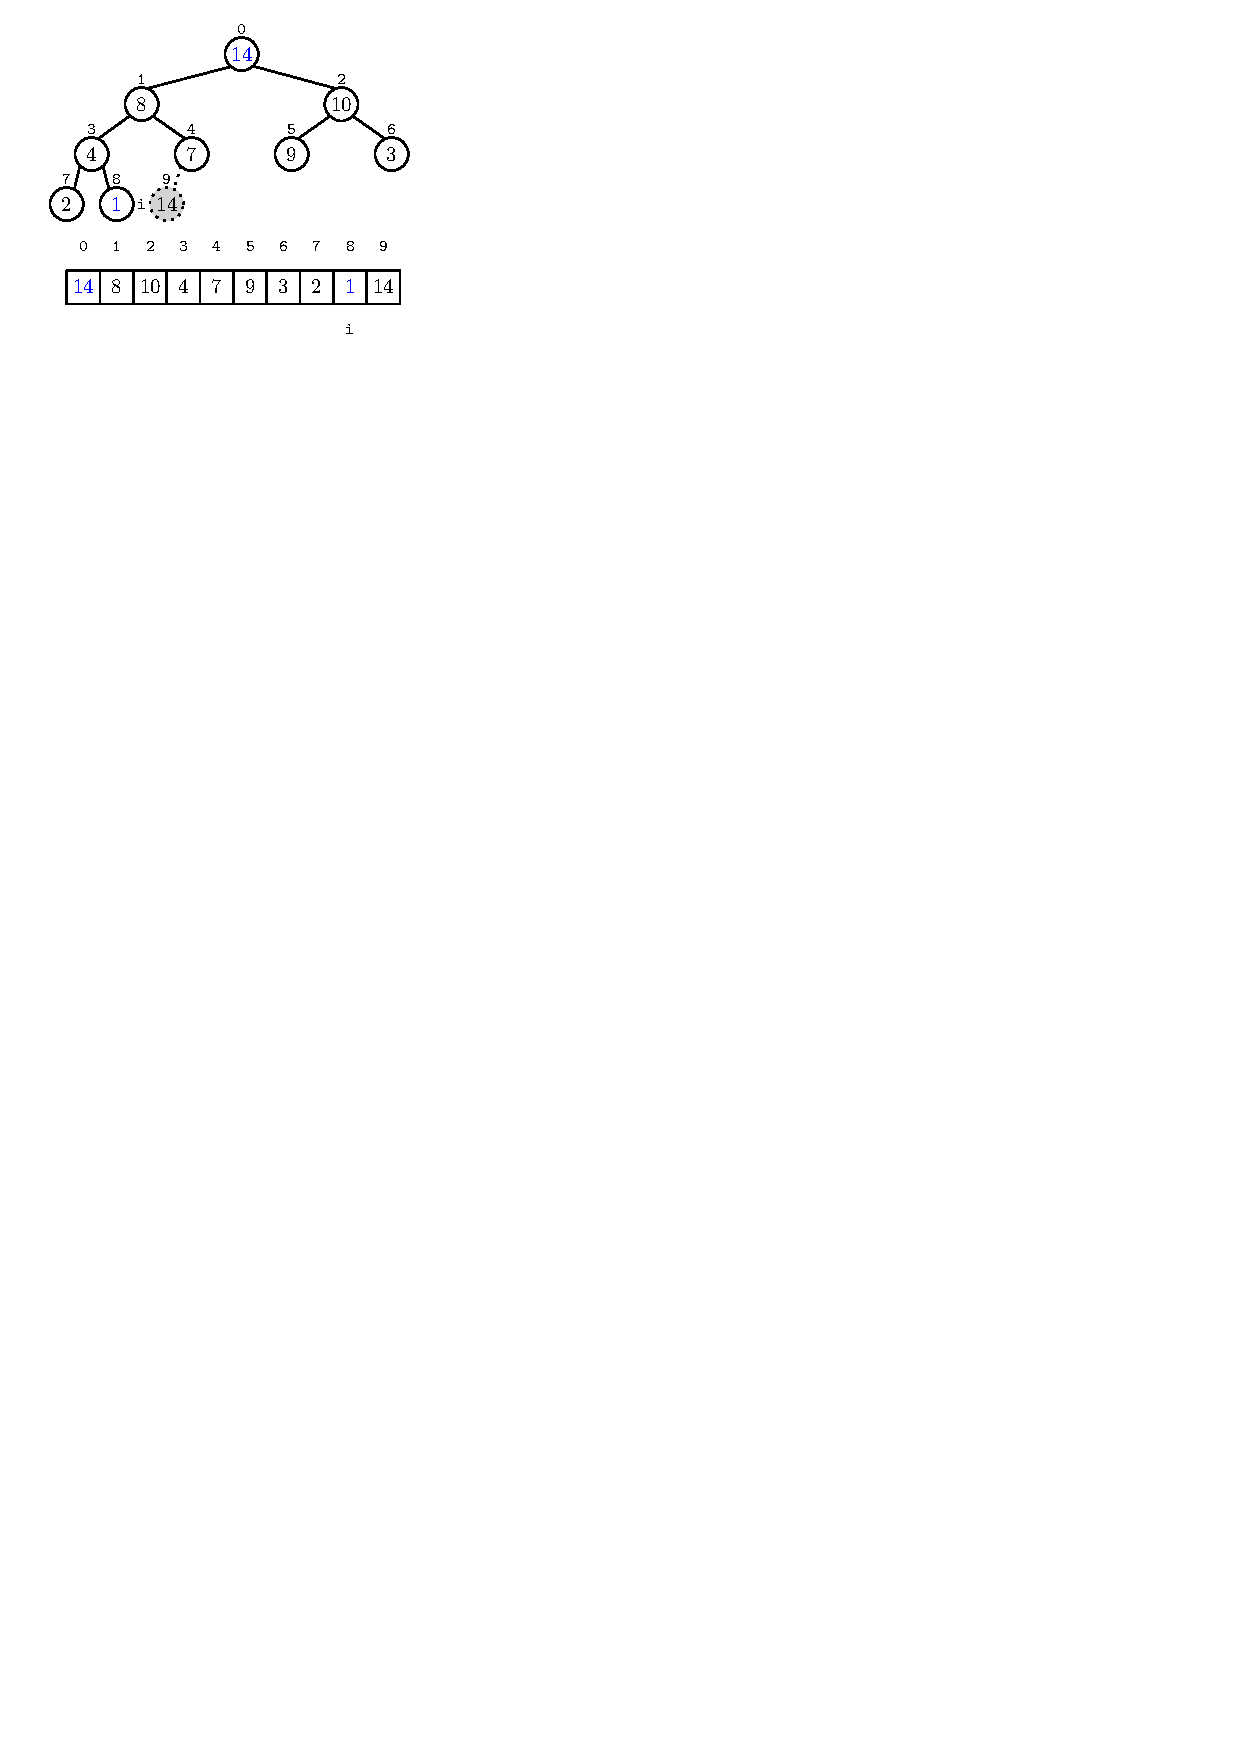
\includegraphics[width=0.8\textwidth]{img/img22.pdf}};
        \node<4> (i4) {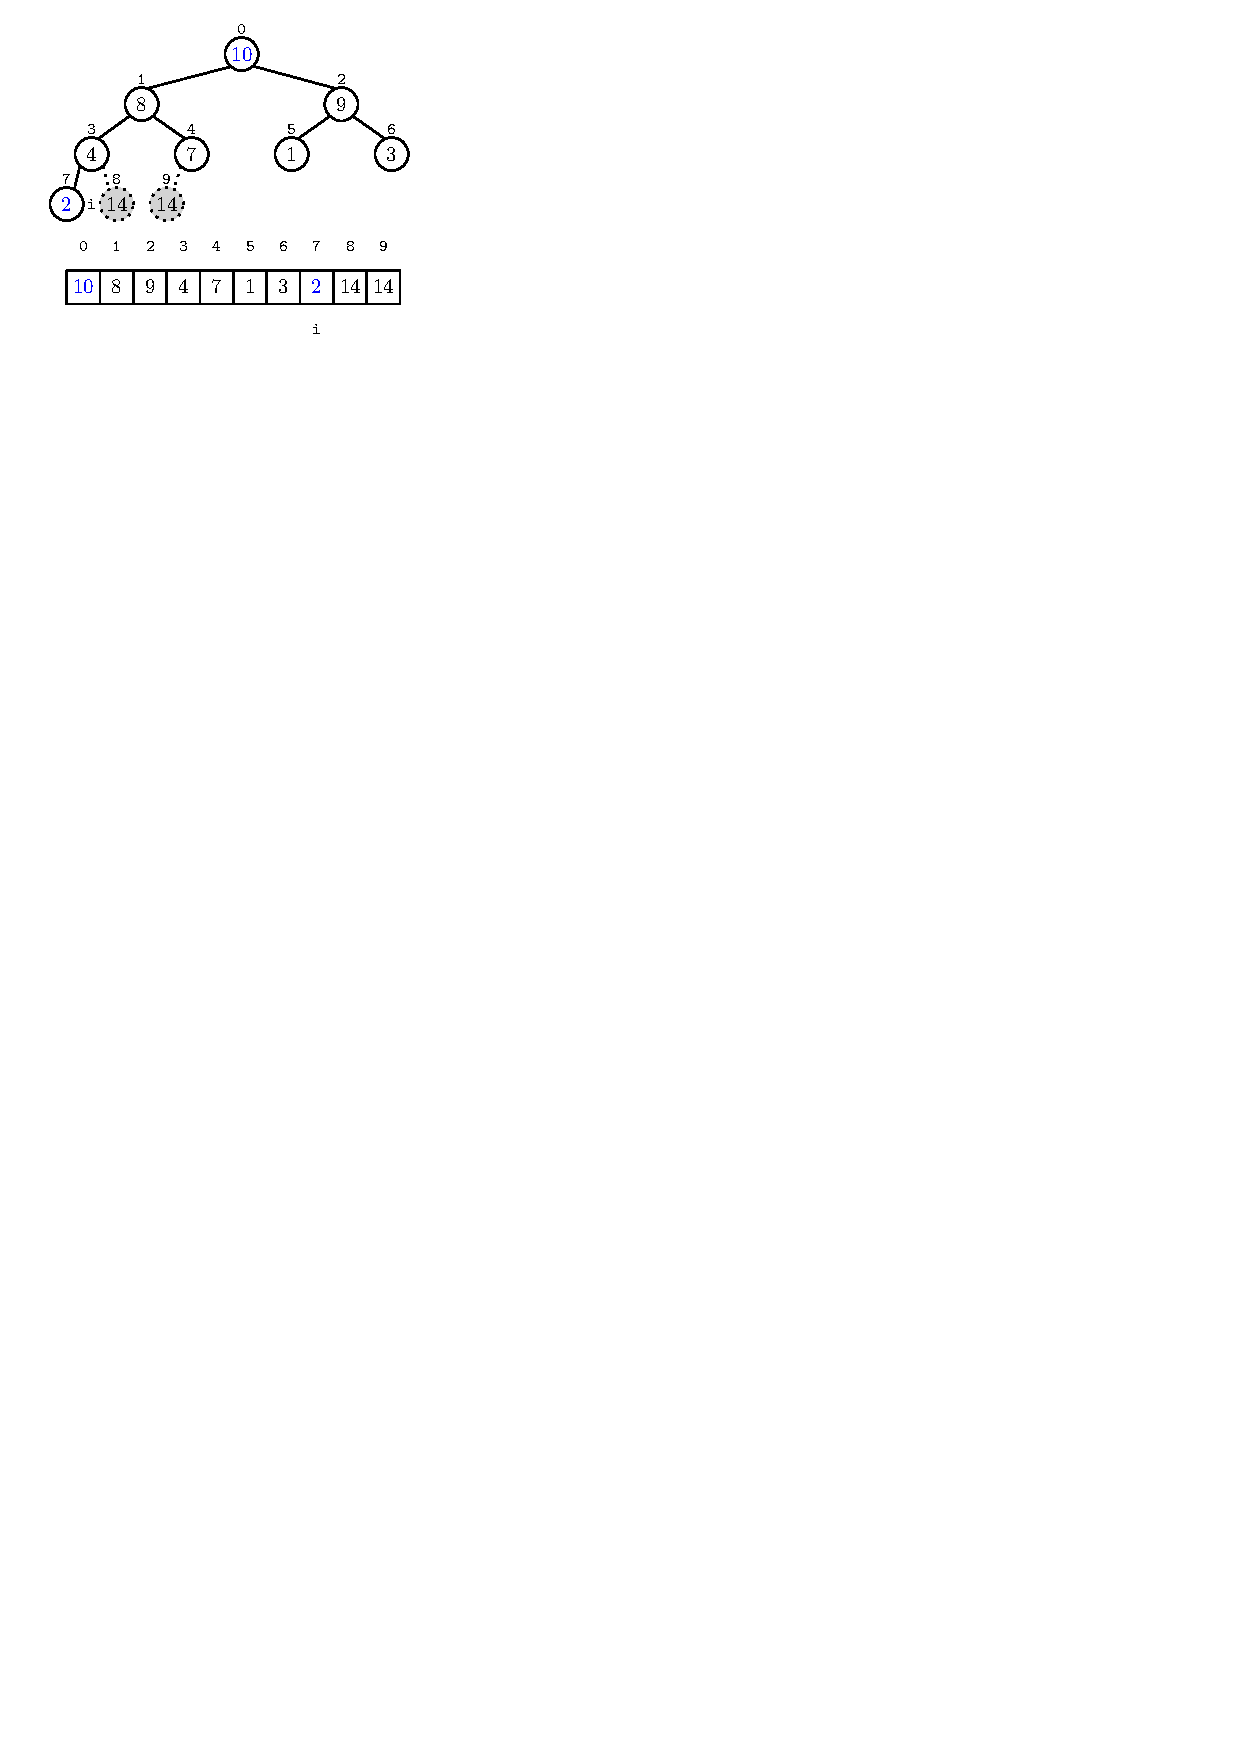
\includegraphics[width=0.8\textwidth]{img/img23.pdf}};
        \node<5> (i5) {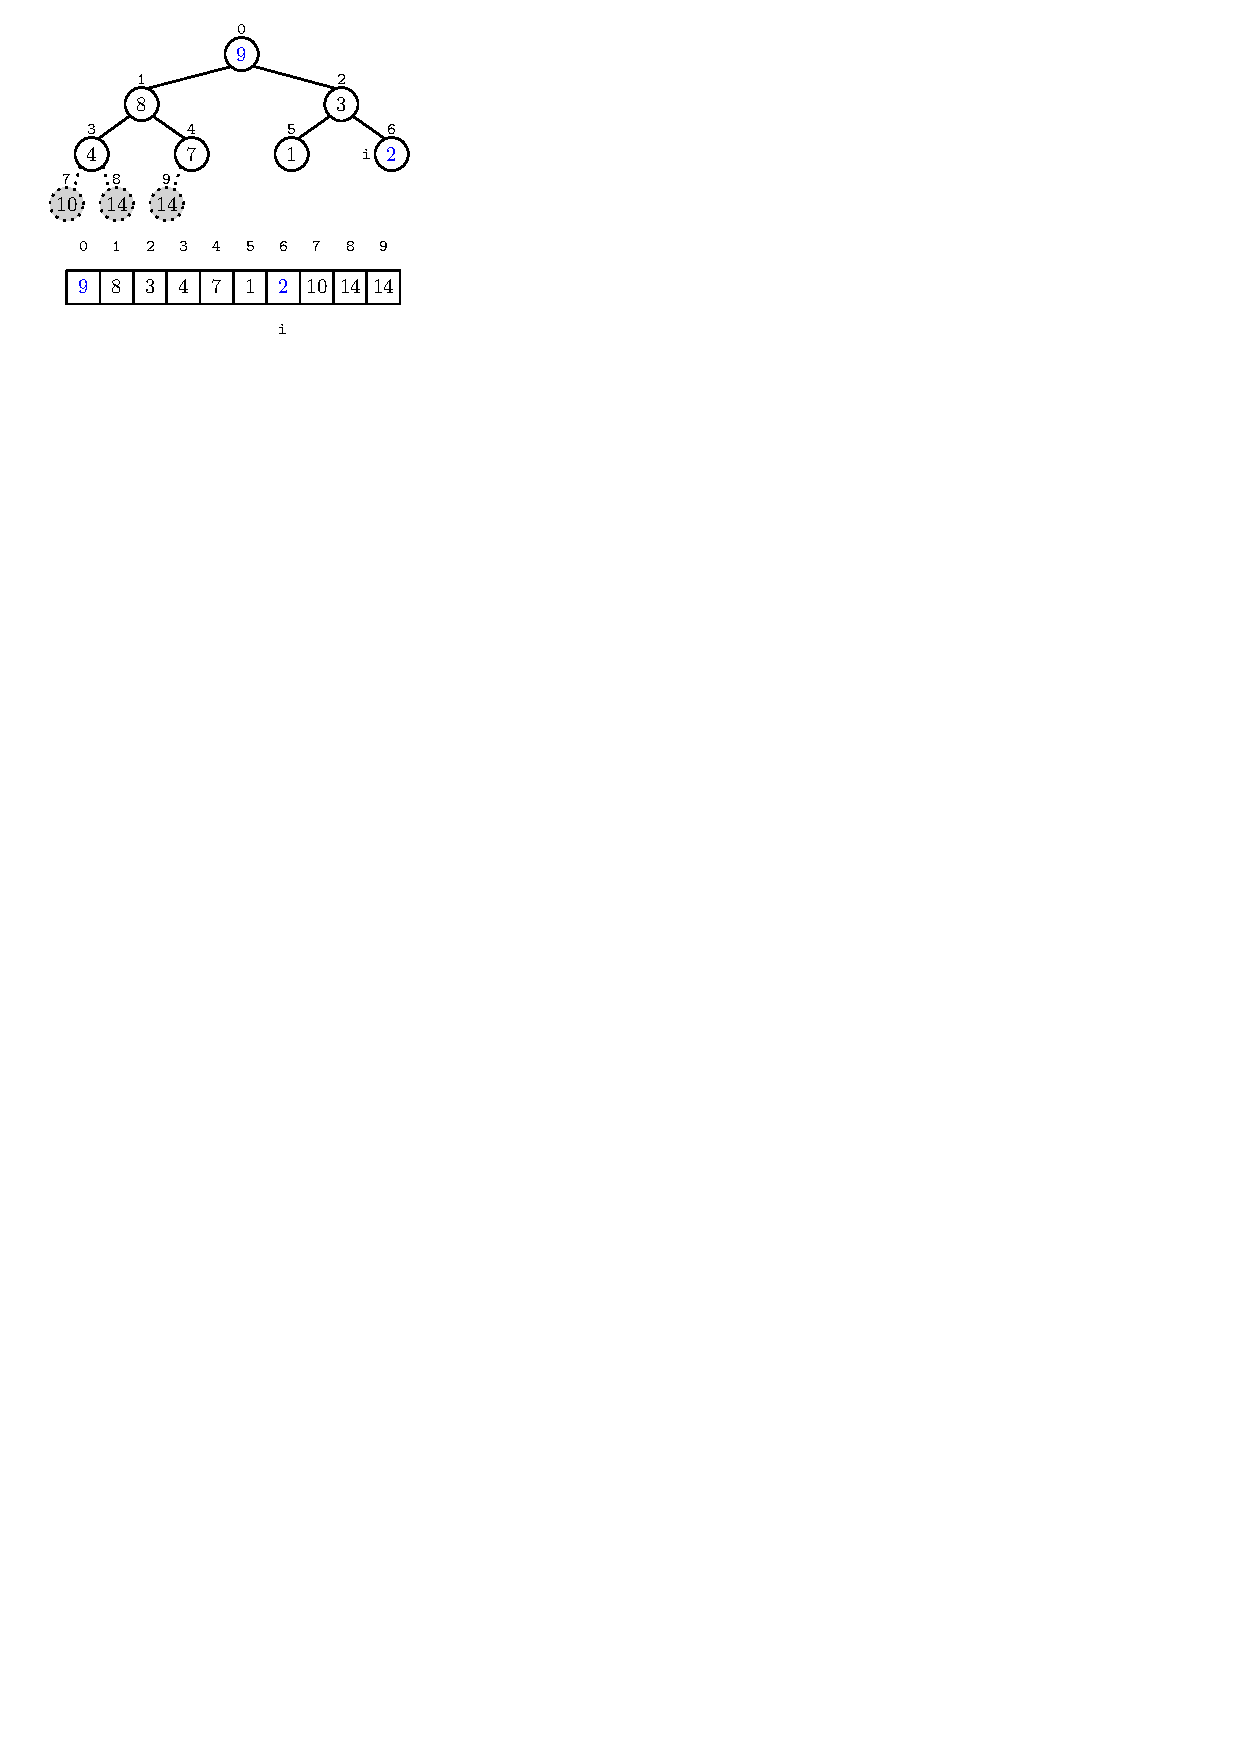
\includegraphics[width=0.8\textwidth]{img/img24.pdf}};
        \node<6> (i6) {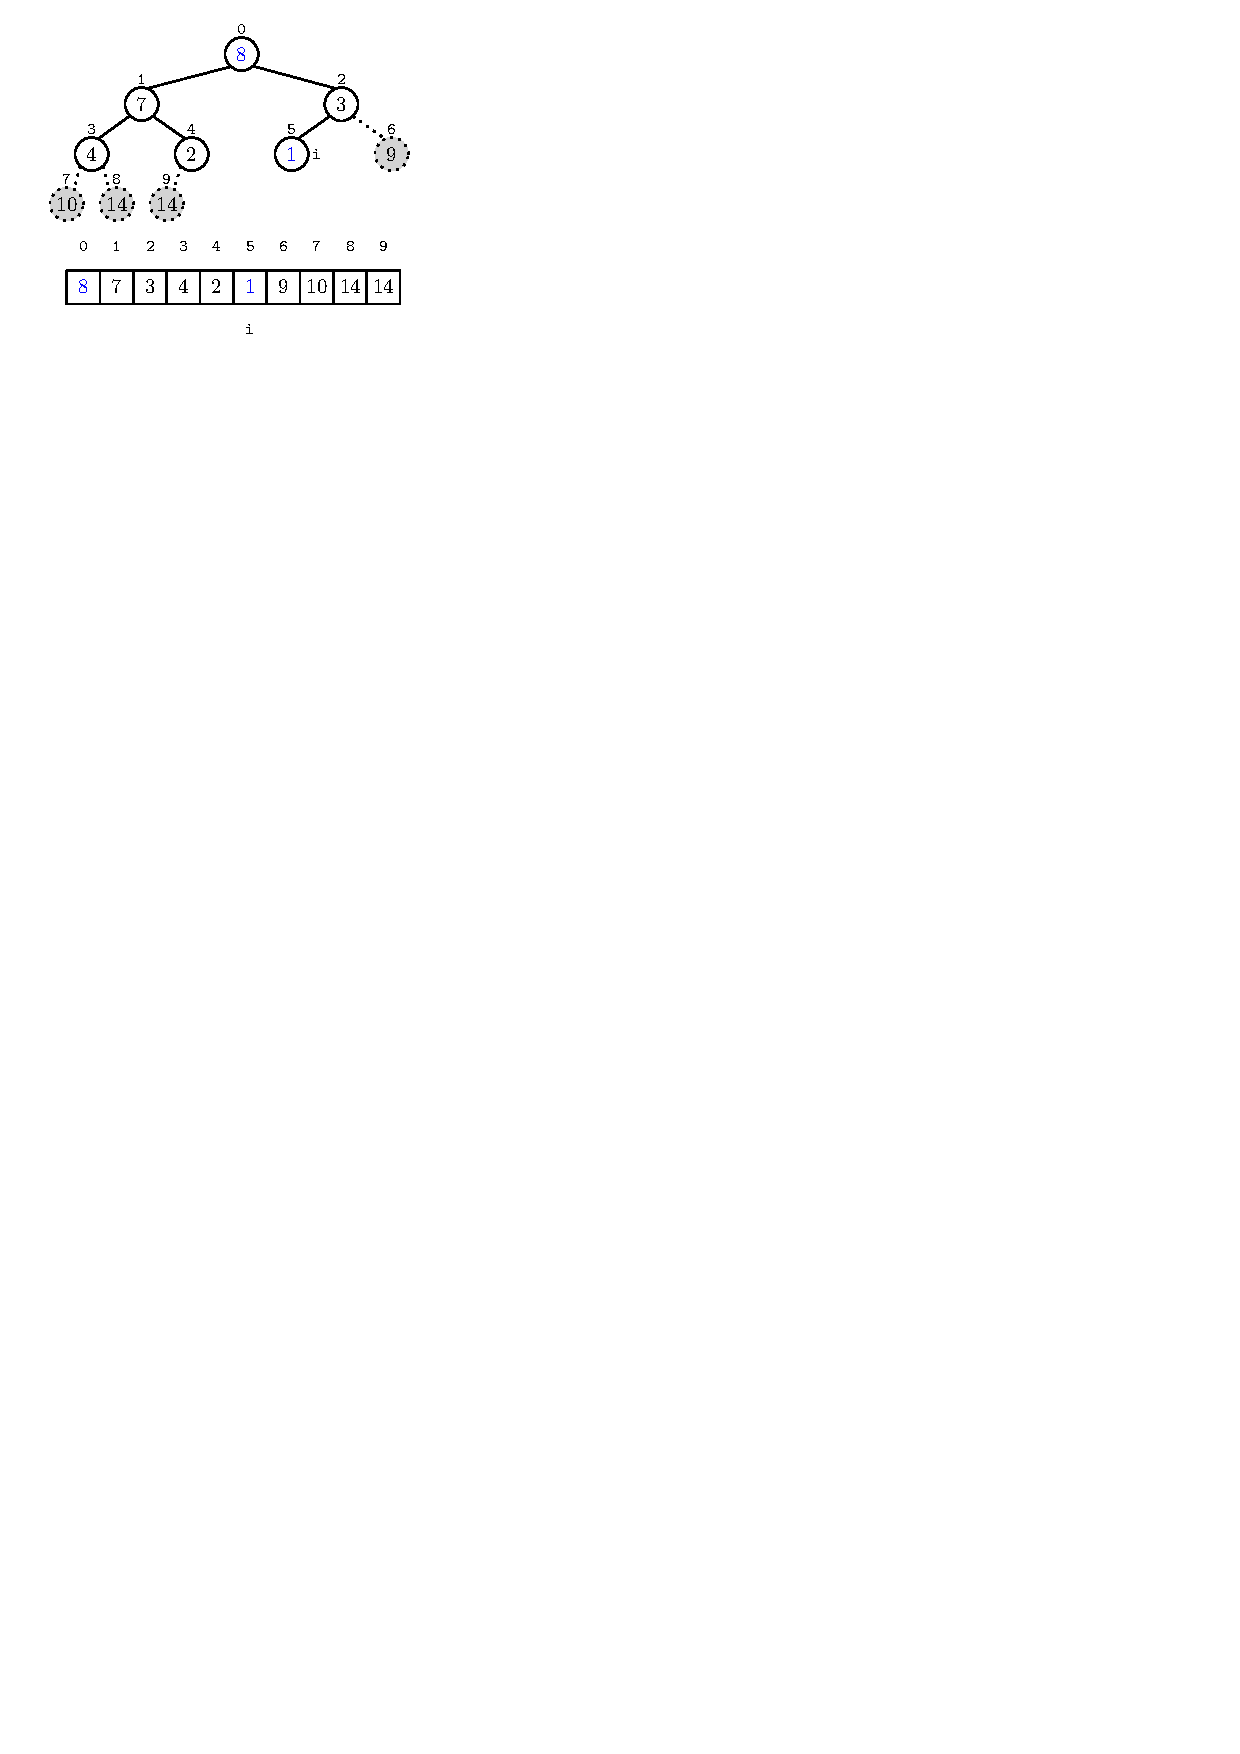
\includegraphics[width=0.8\textwidth]{img/img25.pdf}};
        \node<7> (i7) {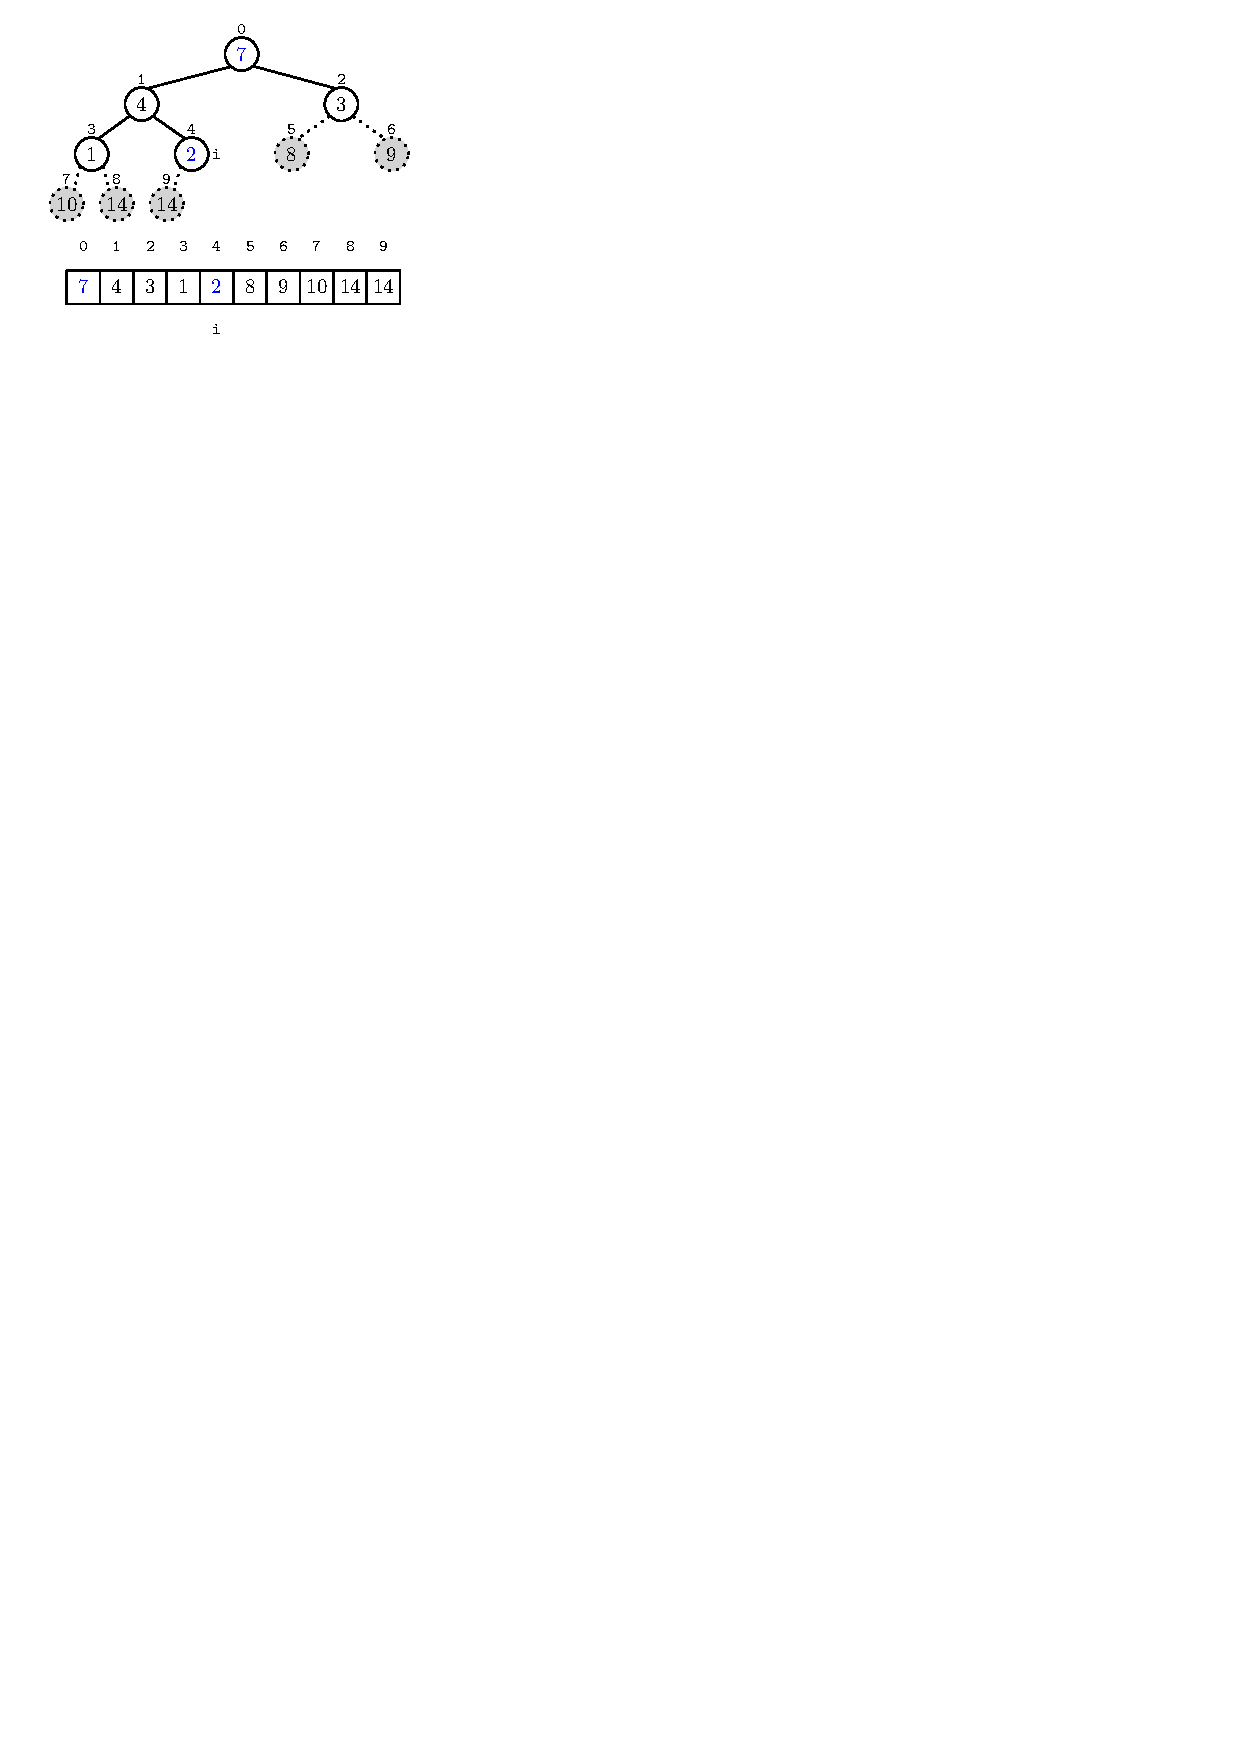
\includegraphics[width=0.8\textwidth]{img/img26.pdf}};
        \node<8> (i8) {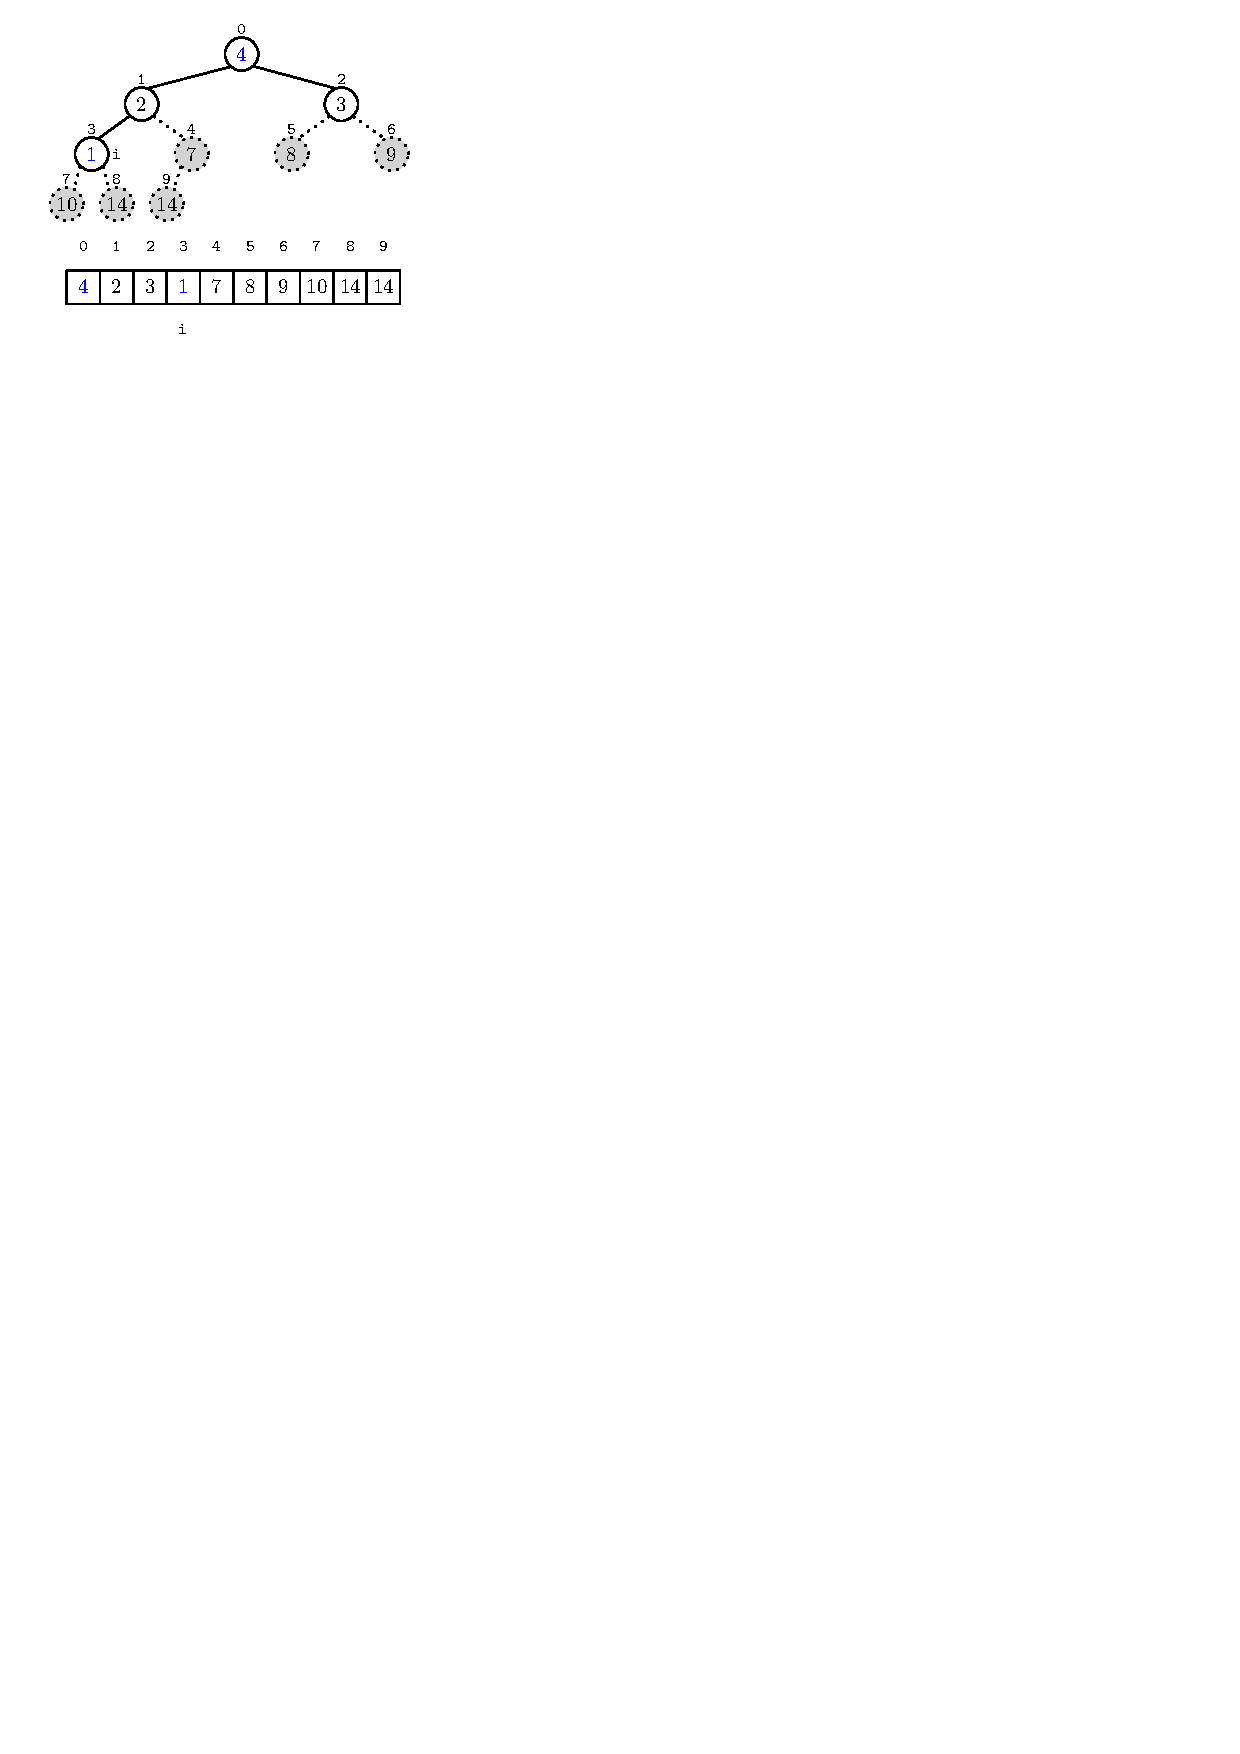
\includegraphics[width=0.8\textwidth]{img/img27.pdf}};
        \node<9> (i9) {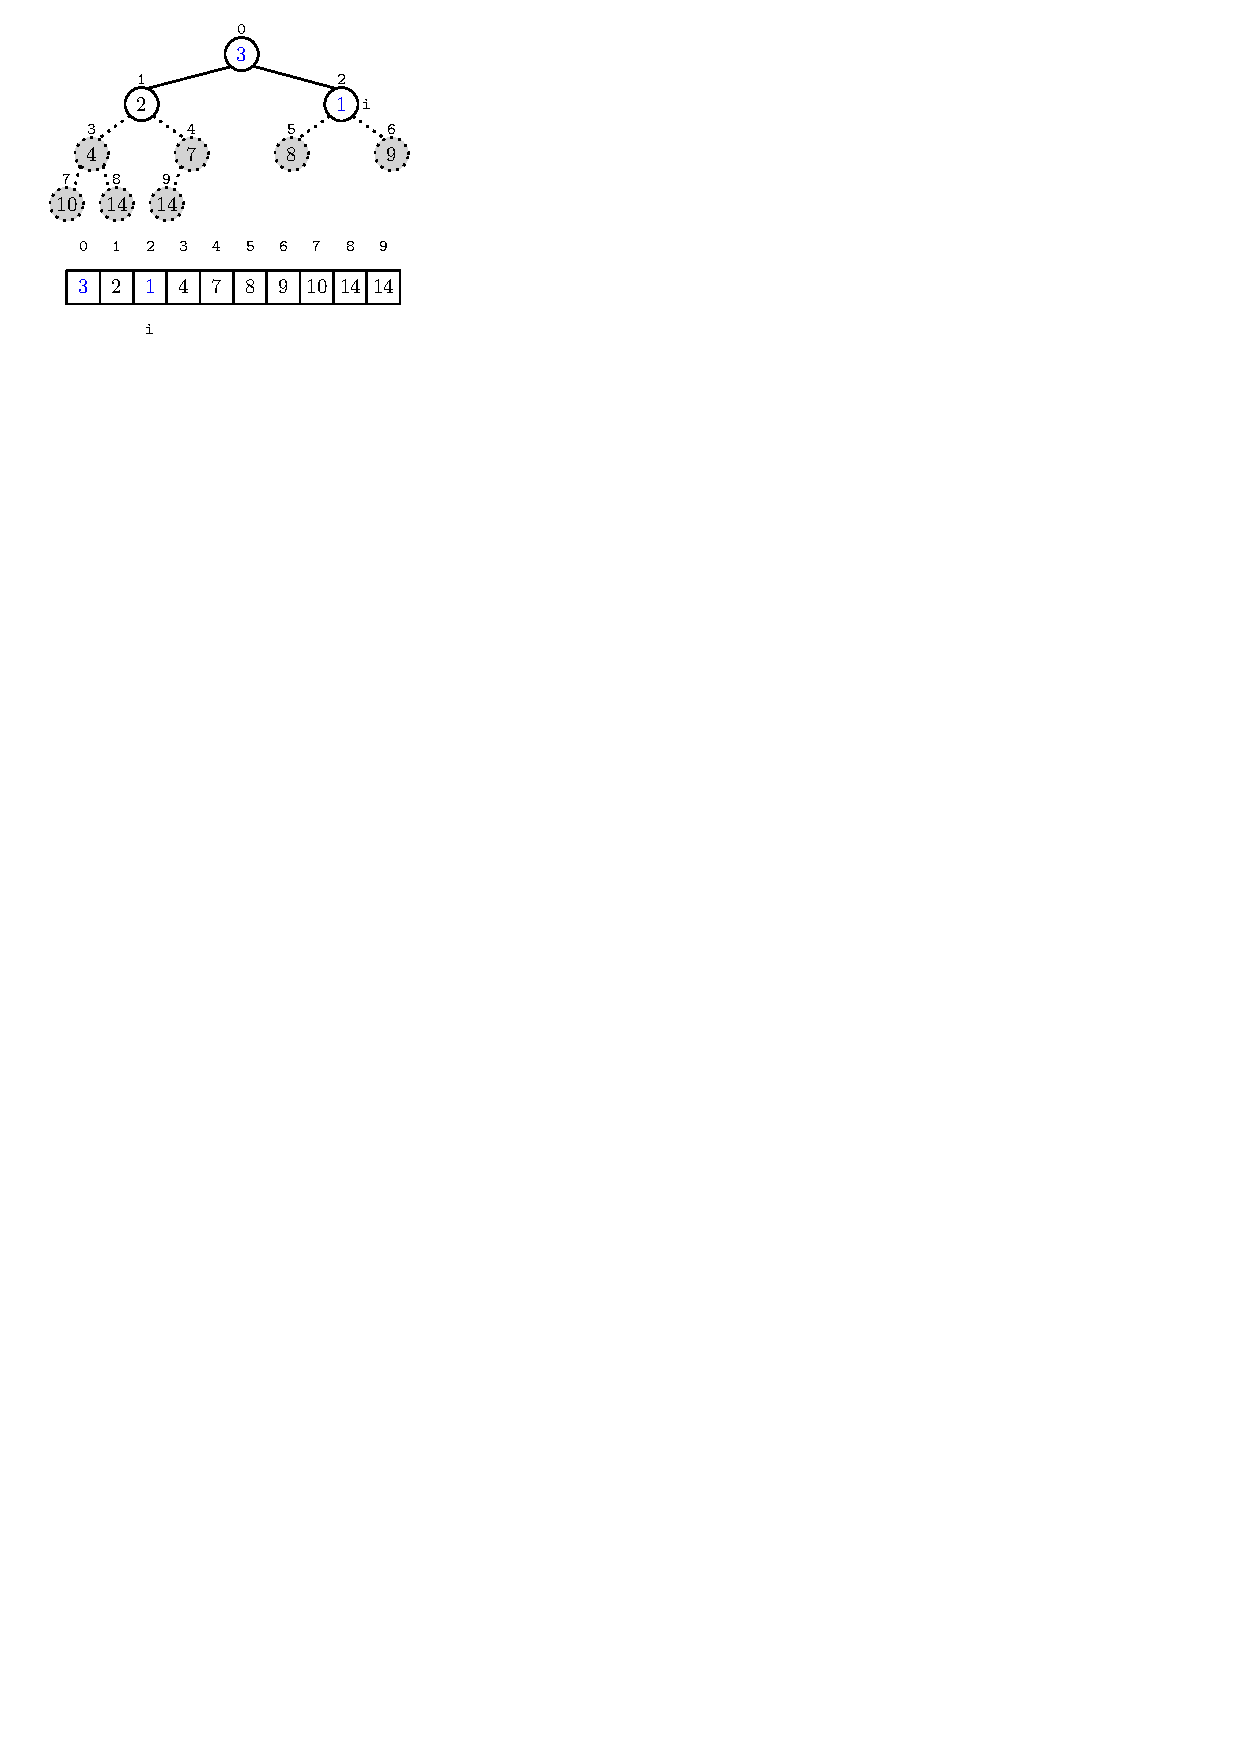
\includegraphics[width=0.8\textwidth]{img/img28.pdf}};
        \node<10> (i10) {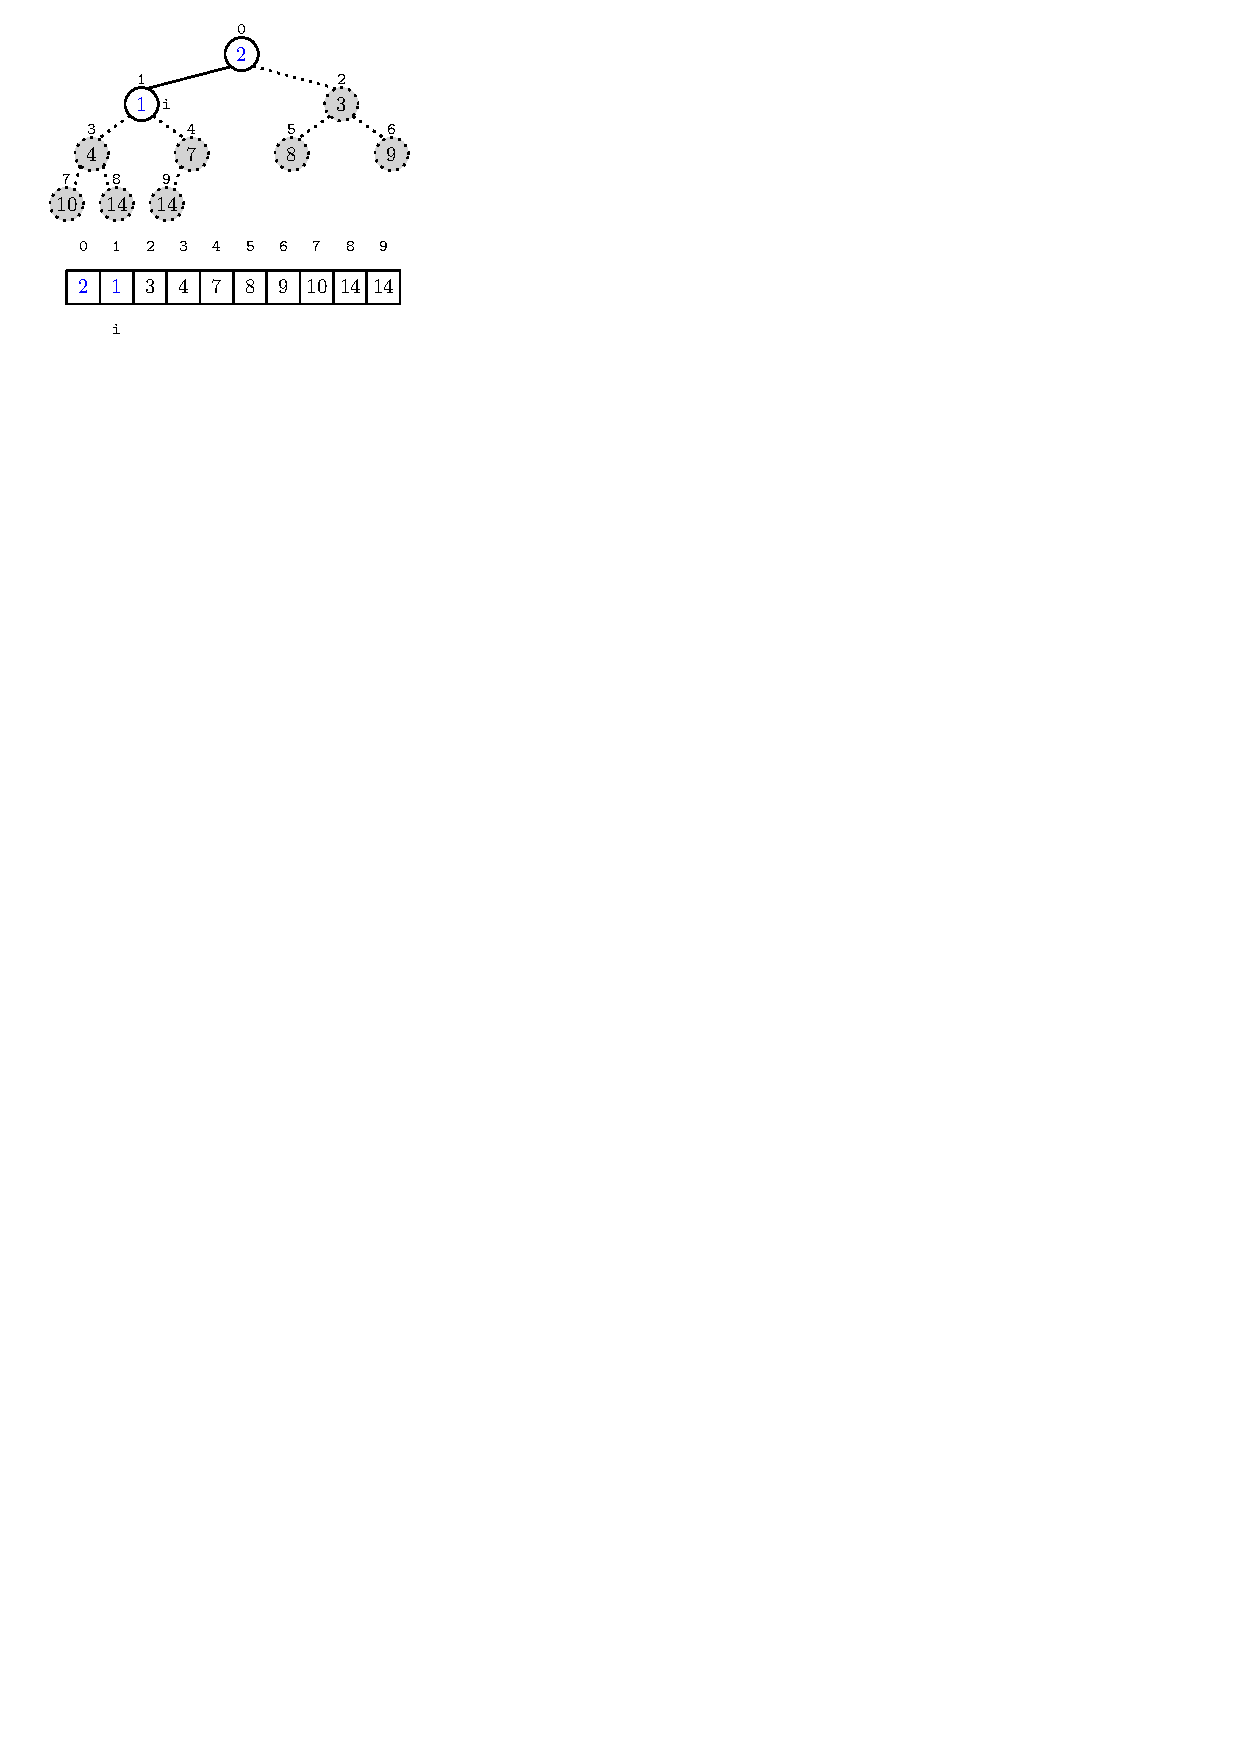
\includegraphics[width=0.8\textwidth]{img/img29.pdf}};
        \node<11> (i11) {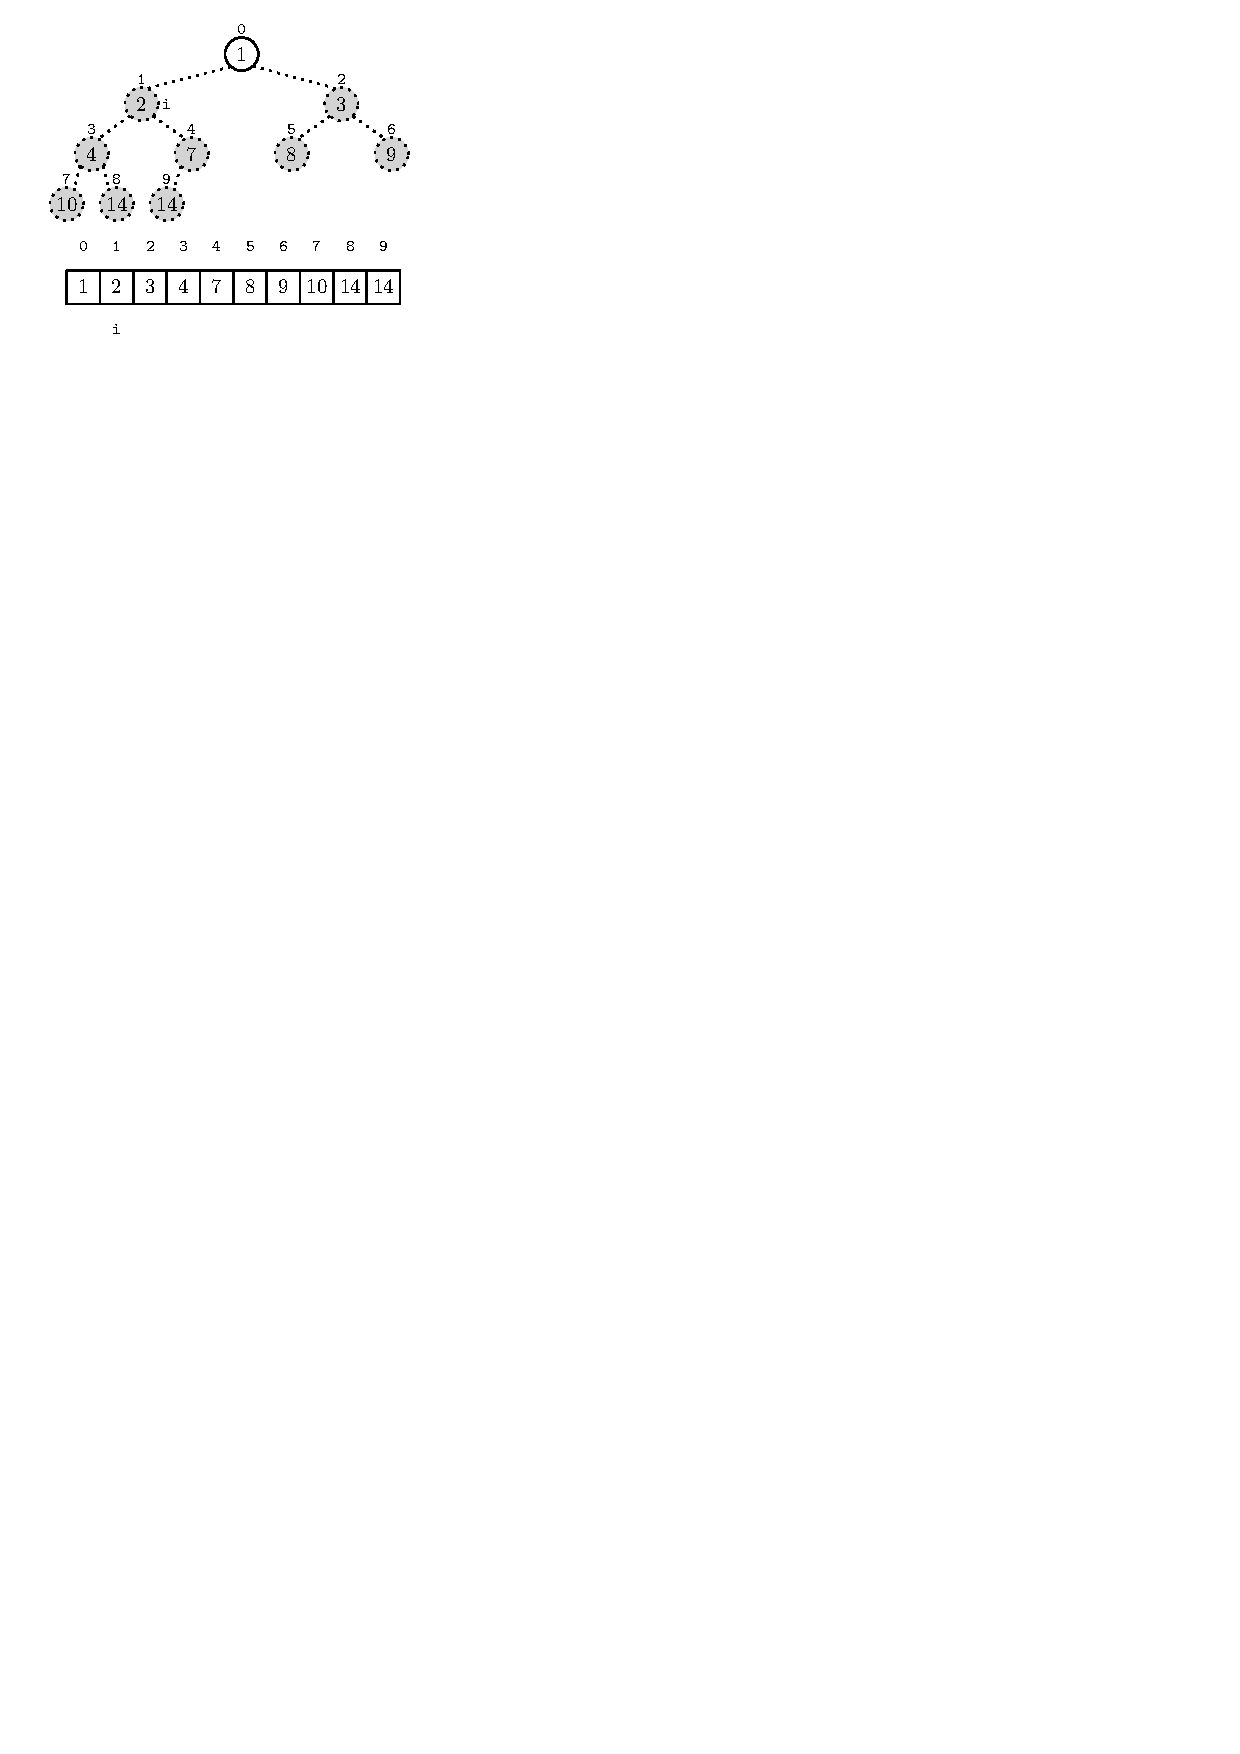
\includegraphics[width=0.8\textwidth]{img/img30.pdf}};
      \end{tikzpicture}
    \end{figure}
  \end{frame}

  \subsection{Implementação}
  \begin{frame}[fragile]{Heap Sort - Implementação}
    \begin{center}
    \begin{minipage}{0.52\textwidth}
    \only<2>{\setminted{highlightlines=4}}
    \only<3>{\setminted{highlightlines=6}}
    \only<4>{\setminted{highlightlines=7-9}}
    \only<5>{\setminted{highlightlines=11}}
    \begin{minted}{c}
    int heapSort (int * v, int n) {
      int comp = 0;
      
      comp = buildMaxHeap(v, n);
      
      for (int i = n - 1; i >= 0; i--) {
        int aux = v[0];
        v[0] = v[i];
        v[i] = aux;
        
        comp += maxHeapify(v, i, 0);
      }
      
      return comp;
    }
    \end{minted}
    \end{minipage}
    \end{center}

    \vspace{-0.5em}
    \begin{enumerate}
      \item<2-> Construir um \emph{heap} máximo;
      \item<3-> Percorrer o heap de trás pra frente, de $i = n - 1$ até $1$:
      \begin{enumerate}
        \item<4-> Trocar o elemento \texttt{v[0]} com o último, ou seja, \texttt{v[i]}.
        \item<5> Chamar \texttt{maxHeapify} para refazer o \emph{heap} máximo.
      \end{enumerate}
    \end{enumerate}

    \vspace{-0.5em}
    {\only<5>{\scriptsize \url{https://repl.it/@alessandrojean/HeapSortComparison}}}
    
  \end{frame}

  \subsection{Análise do custo}
  \begin{frame}{Heap Sort - Análise do custo}
    \begin{itemize}
      \item A chamada ao \texttt{buildMaxHeap} tem custo $O(n)$;
      \item As $n - 1$ chamadas a \texttt{maxHeapify} tem custo $O(\log(n))$.
    \end{itemize}
    Juntando, temos:
    
    \begin{align*}
      T(n)
      &= O(n) + O((n - 1) \cdot \log(n)) \\
      &= O(n) + O(n \cdot \log(n)) \\
      &= O(n \log(n))
    \end{align*}
  \end{frame}

  \section{Conclusões}
  \begin{frame}{Conclusões}
    \begin{itemize}
      \item Algoritmo instável, com custo $O(n\log(n))$ no pior caso;
      \item Algoritmo in-place, não requer memória auxiliar;
      \item Efetua muitas comparações;
      \item É mais custoso fazer a manutenção do \emph{heap} do que particionar, como
      o Quick Sort, por exemplo.
      \item Pode ordenar um vetor em ordem decrescente, utilizando funções
      para \emph{heaps} mínimos (\textbf{Estudo independente});
      \item Pode ser implementado de baixo para cima, gerando o Bottom-up heapsort com
      custo 0.25 vezes melhor do que o original (\textbf{Estudo independente});
      \item Pode ser combinado com o Quick Sort, gerando o Intro Sort, que obtém as vantagens
      de ambos;
    \end{itemize}
  \end{frame}

  \begin{frame}{Recursos computacionais}
    \begin{itemize}
      \item
      Visualização interativa do algoritmo:
      
      \url{https://visualgo.net/en/heap}

      \item
      Comparação com outros algoritmos:

      \url{http://sorting.at}
      
      \item
      Comparação entre diversas entradas:
      
      \url{http://sorting-algorithms.com}
      
      \item
      Funcionamento em vídeo \textit{(em inglês)}:
      
      \url{https://youtu.be/MtQL_ll5KhQ}
      
      \item
      Animação comparando com o Merge sort \textit{(em inglês)}:
      
      \url{https://youtu.be/H5kAcmGOn4Q}
      
      \item
      Heap sort em 4 minutos \textit{(em inglês)}:
      
      \url{https://youtu.be/2DmK_H7IdTo}
      
      \item
      Aula da UNIVESP sobre Heap sort:
      
      \url{https://youtu.be/KtlWBhaygH8}
      
      \item
      Aula do MIT sobre Heap sort \textit{(em inglês)}:
      
      \url{https://youtu.be/B7hVxCmfPtM}
    \end{itemize}
  \end{frame}

  \begin{frame}{Referências Bibliográficas}
    \begin{itemize}
      \item SEDGEWICK, R. Algorithms in C, Parts 1-4: Fundamentals, Data Structures, Sorting, Searching. 
        Addison-Wesley, 1997.
        
      \item CORMEN, T\@. H\@. et al. Algoritmos: Teoria e Prática. Editora Campus, 2002.
      
      \item RAVULA, R\@. Algorithms lecture 13 - Build max heap algorithm and analysis. 
      Youtube, Julho de 2014. Disponível em: \url{https://youtu.be/HI97KDV23Ig}
      
      \item MOTA, G\@. O. Análise de Algoritmos e Estruturas de Dados: Notas de aula. 2018.
    \end{itemize}
  \end{frame}

  \begin{frame}{Referências Bibliográficas}
    \begin{itemize}      
      \item MENA-CHALCO, J\@. P. Heap Sort. 2017. 65 slides. \footnotemark[1]
      
      {\vspace{-0.5em}\fontsize{6pt}{1pt}\selectfont \url{http://professor.ufabc.edu.br/~jesus.mena/courses/mcta001-1q-2017/AED1-10.pdf}}
      
      \item RIBEIRO, M\@. P. Ordenação Heaps binários. 2018. 78 slides. \footnotemark[1]
      
      {\vspace{-0.5em}\fontsize{6pt}{1pt}\selectfont \url{https://drive.google.com/file/d/1kA4ijg20vshT-b_RUFEV3mIBZZ2_aVGW/view}}
      
      \item BUENO, L\@. R. Heapsort. 2013. 62 slides. \footnotemark[1]
      
      {\vspace{-0.5em}\fontsize{6pt}{1pt}\selectfont \url{http://professor.ufabc.edu.br/~leticia.bueno/classes/aa/materiais/heapsort.pdf}}
      
      \item SOUZA, J\@. F\@. de. HeapSort. 2009. 46 slides. \footnotemark
      
      {\vspace{-0.5em}\fontsize{6pt}{1pt}\selectfont \url{http://www.ufjf.br/jairo_souza/files/2009/12/2-Ordenação-HeapSort.pdf}}
      
      \item SANTI, J. Heap e Heap-Sort. 2017. 127 slides. \footnotemark
    \end{itemize}

    \footnotetext[1]{
      Material apresentado para a disciplina de Algoritmos e Estruturas de Dados I no curso
      de Ciência da Computação da UFABC.
    }
    \footnotetext[2]{
      Material apresentado para a disciplina de Estrutura de Dados II no curso
      de Ciência da Computação da UFJF.
    }
    \footnotetext[3]{
      Material apresentado para a disciplina de Estrutura de Dados II no curso de
      Sistemas de Informação da UTFPR.
    }
  \end{frame}

  \begin{frame}[plain, c]
    \begin{center}
      
\includegraphics[scale=0.3]{img/github-icon.pdf}
        
      Material disponível no GitHub.
    
      {\footnotesize \url{https://github.com/alessandrojean/AED-I-2018.1}}
      
      {\footnotesize \url{https://repl.it/@alessandrojean/HeapSort}}
    \end{center}
  \end{frame}

\end{document}